% !Mode::"Tex:UTF-8"
\documentclass[UTF8,a4paper,titlepage]{ctexart}
\usepackage{listings}
\usepackage{xcolor}
\usepackage{setspace}
\usepackage{float}
\usepackage{fontspec}
\usepackage{geometry}
\usepackage{hyperref}
\usepackage{tabularx}
\usepackage{amsmath}
\usepackage{graphicx}

\geometry{left=1.5cm,right=1.5cm,top=2.5cm,bottom=2.5cm}
\newfontfamily\cn{Courier New}
\setcounter{tocdepth}{4}
\lstset{
%numbers=left, %左侧行号
%numberstyle= \footnotesize, 
basicstyle=\linespread{0.8}\small\cn,
keywordstyle=\bfseries\color{blue},
commentstyle=\color{gray}\songti,
%stringstyle=
%frame=shadowbox, 
rulesepcolor= \color{red!20!green!20!blue!20},
escapeinside=``,
xleftmargin=2em,
xrightmargin=2em,
aboveskip=1em}


\title{BNU Faraway模板库}
\author{SK}
\date{\today}
\begin{document}
\maketitle
\tableofcontents
\section{DP}
\subsection{整数划分}
\begin{lstlisting}[language=C++]
/*
f[n][m]将n划分为不超过m个数的方案数
6
6;
5+1;
4+2;4+1+1;
3+3;3+2+1;3+1+1+1;
2+2+2;2+2+1+1;2+1+1+1+1;
1+1+1+1+1+1;
*/
#define N 45
int n;
int f[N][N];
int work(int n,int m)
{
    if(n==1 || m==1) return f[n][m]=1;
    if(n<m) return f[n][m]=work(n,n);
    if(n==m) return f[n][m]=1+work(n,n-1);
    return f[n][m]=work(n,m-1)+work(n-m,m);
}
int main()
{
    memset(f,-1,sizeof(f));
    while(scanf("%d",&n)!=EOF)
    {
        printf("%d\n",work(n,n));
    }
}
\end{lstlisting}
\subsection{扔蛋问题}
\begin{lstlisting}[language=C++]
/*
有一栋楼共100层,一个鸡蛋从第N层及以上的楼层落下来会摔破, 
在第N层以下的楼层落下不会摔破。给你2个鸡蛋,设计方案找出N,
并且保证在最坏情况下, 最小化鸡蛋下落的次数。(
假设每次摔落时,如果没有摔碎,则不会给鸡蛋带来损耗)
答案是14
本题用dp求n层楼,k个鸡蛋的答案
*/
#include<cstring>
#include<iostream>
#include<cstdio>
#include<algorithm>
using namespace std;
int dp[1005][55];
void pre()
{
    for(int i=0;i<=1000;++i)
    {
        dp[i][0]=0;
        dp[i][1]=i;
    }
    for(int i=2;i<=50;++i)
    {
        dp[0][i] = 0;
        dp[1][i] = 1;
    }
    for(int i=2;i<=1000;++i)
        for(int j=2;j<=50;++j)
        {
            dp[i][j]=~0U>>1;
            for(int k=1;k<=i;k++)
                dp[i][j]=min(dp[i][j],max(dp[i-k][j],dp[k-1][j-1])+1);
        }
}
int main()
{
    pre();
    int sk;
    scanf("%d",&sk);
    for(int cas=1; cas<=sk; cas++)
    {
        int n,k;
        scanf("%d%d",&k,&n);
        printf("Case %d: %d\n",cas,dp[n][k]);
    }
}
\end{lstlisting}
\subsection{多重背包+二进制优化+bitset优化}
\begin{lstlisting}[language=C++]
/* fjnu 1197 */
#include<cstring>
#include<cstdio>
#include<iostream>
#include<algorithm>
#include<bitset>
using namespace std;
bitset<10005> dp;
int num[15];
int sum[2];
int n;
int cost[1005],f[1005];
int x,y;
void pack(int val)
{
    dp=dp|(dp<<val);
}
void multi(int val,int num)
{
    int k=1;
    while(k<=num)
    {
        pack(val*k);
        num-=k;
        k*=2;
    }
    pack(val*num);
}
int main()
{
    int sk;
    scanf("%d",&sk);
    while(sk--)
    {
        memset(num,0,sizeof(num));
        sum[0]=sum[1]=0;
        scanf("%d",&n);
        for(int i=1; i<=n; i++)
        {
            scanf("%d%d",cost+i,f+i);
            sum[f[i]]+=cost[i];
            num[cost[i]]++;
        }
        if(sum[0]>=sum[1])
        {
            printf("%d\n",sum[0]);
        }
        else
        {
            dp.reset();
            dp[0]=1;
            for(int i=1; i<=10; i++)
                multi(i,num[i]);
            int ans=~0U>>1;
            for(int i=0; i<=sum[0]+sum[1]; i++)
                if(dp[i])
                    ans=min(ans,max(i,sum[0]+sum[1]-i));
            printf("%d\n",ans);
        }
    }
}

       \end{lstlisting}
\subsection{最长上升子序列}
\begin{itemize}
	\item 严格上升lower\_bound,非严格上升upper\_bound
	\item 也可以用求前缀最值的树状数组
	\item Dilworth定理:对于一个偏序集,最少链划分等于最长反链长度,也就是说把一个数列划分成最少的最长不升子序列的数目就等于这个数列的最长上升子序列的长度。
\end{itemize}
\begin{lstlisting}[language=C++]
int main()
{
    int sk;
    scanf("%d",&sk);
    while(sk--)
    {
        int ans=0;
        scanf("%d",&n);
        for(int i=1;i<=n;i++)
        {
            int x;
            scanf("%d",&x);
            int j=lower_bound(b+1,b+ans+1,x)-b;
            if(j>ans) b[++ans]=x;
            else b[j]=x;
        }
        printf("%d\n",ans);
    }
}
       \end{lstlisting}
\subsection{最长公共子序列 优化}
\begin{itemize}
	\item ICPCCAMP2017 DAY4 B,时间复杂度$O(26n+m^2)$
	\item dp(i, j) 表示第二个串前i个字符与第一个串前dp(i,j)个字符的LCS至少为j,且dp(i, j) 为满足条件的最小值。假设已知dp(i,j),考虑转移到第二个串的第i + 1 个位置,如果该位置不对LCS产生贡献,则直接转移到dp(i + 1, j);否则在第一个串的dp(i, j) 位置后找到第一个匹配的字符位置转移到dp(i + 1, j + 1)。
	\item 和LCS的优化类似,\textbf{启示是将原dp状态和dp的值交换一下},变成求当前dp值下的最优的一个决策。
\end{itemize}
\begin{lstlisting}[language=C++]
/**/
#include<bits/stdc++.h>
#define rep(i,a,b) for (int i=(a);i<(b);i++)
#define per(i,a,b) for (int i=(b)-1;i>=(a);i--)
using namespace std;
int n,m;
char s[1010000],t[1010];
int nxt[1010000][26],dp[1010][1010];
int main()
{
    int te;
    scanf("%d",&te);
    while(te--)
    {
        scanf("%s%s",s+1,t+1);
        n=strlen(s+1);
        m=strlen(t+1);

        rep(i,0,26) nxt[n+1][i]=n+1;
        per(i,1,n+1)
        {
            rep(j,0,26) nxt[i][j]=nxt[i+1][j];
            nxt[i][s[i]-'a']=i;
        }

        rep(i,0,m+1) rep(j,0,i+1) dp[i][j]=n+1;
        dp[0][0]=0;
        rep(i,0,m)
            rep(j,0,i+1)
            if (dp[i][j]<=n)
            {
                dp[i+1][j]=min(dp[i+1][j],dp[i][j]);
                dp[i+1][j+1]=min(dp[i+1][j+1],nxt[dp[i][j]+1][t[i+1]-'a']);
            }
        int ans=0;
        rep(j,0,m+1) if (dp[m][j]<=n) ans=j;
        printf("%d\n",ans);
    }
    return 0;
}
      \end{lstlisting}
\subsection{数位dp}
\begin{lstlisting}[language=C++]
/*
不要62和4
*/
#include<bits/stdc++.h>
using namespace std;
int b[20];
int dp[20][2];
int dfs(int pos, int preok, int pre6)
{
    if (pos==-1) return 1;
    if (preok && dp[pos][pre6]!=-1) return dp[pos][pre6];
    int up = preok? 9 : b[pos];
    int sum = 0;
    for (int i=0; i<=up; i++) {
        if (i!=4 && !(pre6&&i==2)) {
            sum += dfs(pos-1, preok||i<b[pos], i==6);
        }
    }
    if (preok) dp[pos][pre6] = sum;
    return sum;
}
int solve(int R)
{
    int cnt = 0;
    while (R) {
        b[cnt++] = R % 10;
        R /= 10;
    }
    return dfs(cnt-1, 0, 0);
}
int main()
{
    memset(dp, -1, sizeof(dp));
    int n, m;
    while (~scanf("%d%d", &n, &m) && n||m) {
        printf("%d\n", solve(m) - solve(n-1));
    }
    return 0;
}
      \end{lstlisting}
\subsection{树形dp}
\begin{lstlisting}[language=C++]
/*
01分数规划+树形dp
dp[i][j]表示以i为根的联通块大小为j的最大点权和
O(n^2)的时间复杂度
*/
#include<bits/stdc++.h>
using namespace std;
#define N 2550
const double INF=1e99;
int k,n;
int num[N],a[N],b[N];
double dp[N][N],c[N];
vector<int> e[N];

void dfs(int u,int f)
{
    double tmp[N];
    tmp[0]=c[u];
    num[u]=0;
    for(auto &v:e[u])
    {
        if(v==f)continue;
        dfs(v,u);
        double now[N];
        for(int i=0;i<=num[u]+num[v];i++)
            now[i]=-INF;
        for(int i=0;i<=num[u];i++)
            for(int j=0;j<=num[v];j++)
                now[i+j]=max(now[i+j],tmp[i]+dp[v][j]);
        for(int i=0;i<=num[u]+num[v];i++)
            tmp[i]=now[i];
        num[u]+=num[v];
    }
    num[u]++;
    dp[u][0]=0;
    for(int i=1;i<=num[u];i++)
        dp[u][i]=tmp[i-1];
}
double calc(double mid)
{
    c[0]=0;
    for(int i=1;i<=n;++i) c[i]=a[i]-mid*b[i];
    dfs(0,-1);
    return dp[0][k+1];
}
int main()
{
    scanf("%d%d",&k,&n);
    for(int i=1;i<=n;++i)
    {
        int fa;
        scanf("%d%d%d",b+i,a+i,&fa);
        e[fa].push_back(i);
    }
    double l=0,r=10000;
    for(int i=1;i<=50;++i)
    {
        double mid=(l+r)/2;
        if(calc(mid)>=0) l=mid;
        else r=mid;
    }
    printf("%.3f\n",l);
    return 0;
}
      \end{lstlisting}
\subsection{斜率优化 单调队列}
\begin{itemize}
	\item $f[i]=min(f[j]+(sum[i]-sum[j]+i-j-1-L)^2) (0\le j<i)$
	\item 把i-j弄到sum里,-1弄到L里,简化为$f[i]=min(f[j]+(sum[i]-sum[j]-L)^2) (0\le j<i)$
	\item 设j<k<i,且对于i来说,k决策点比j优,则有$\frac{(f[j]+(sum[j]+L)^2)-(f[k]+(sum[k]+L)^2)}{sum[j]-sum[k]} \le 2*sum[i]$
	\item 维护一个斜率递增的单调队列,不等式右边关于i单增,会造成队首出队
\end{itemize}
\begin{lstlisting}[language=C++]
typedef long long ll;
#define N 50010
ll dp[N],sum[N],q[N];
int n;
ll L;
ll sqr(ll x) { return x*x; }
ll Y(int j) { return dp[j]+sqr(sum[j]+L); }
ll X(int j) { return sum[j]; }
ll getup(int j,int k) { return Y(j)-Y(k); }
ll getdown(int j,int k){ return X(j)-X(k); }
ll getdp(int j,int i){ return dp[j]+sqr(sum[i]-sum[j]-L); }
int main(){
    scanf("%d%lld",&n,&L);
    L++;
    for(int i=1;i<=n;++i) {
        scanf("%lld",&sum[i]);
        sum[i]+=sum[i-1]+1;
    }
    int l=0,r=0,x,y,z;
    for(int i=1;i<=n;++i){
        while(l<r && getup(q[l],q[l+1])>=2LL*sum[i]*getdown(q[l],q[l+1])) l++;
        q[++r]=i;
        dp[i]=getdp(q[l],i);
        while(l<=r-2){
            x=q[r-2];y=q[r-1];z=q[r];
            if ((getup(y,x)*getdown(z,y)>=getup(z,y)*getdown(y,x))) q[r-1]=q[r],--r;
            else break;
        }
    }
    cout<<dp[n]<<endl;
    return 0;
}

      \end{lstlisting}

\subsection{斯坦纳树}
\begin{itemize}
	\item 最优解必然是一棵树,状态压缩,dp[i][j]表示以i为根和对应状态为j的节点连通的子树的
	      最小权值。有两种转移。
	\item 枚举子树的形态,即枚举子集:dp[i][j]=min{ dp[i][j],dp[i][k]+dp[i][l] },其中k和l是对j的一个划分。
	\item 按照边进行松弛,用spfa:dp[i][j]=min{ dp[i][j],dp[i'][j]+w[i][i'] },其中i和i'之间有边相连。
	\item 时间复杂度,枚举子集$O(n\times 3^k)$,spfa$O(n\times 2^k)$。
\end{itemize}
\begin{lstlisting}[language=C++]
/*bzoj4006 [JLOI2015]管道连接*/
#include<cstring>
#include<cstdio>
#include<iostream>
#include<algorithm>
#include<queue>
using namespace std;
#define N 1010
const int INF=0x3f3f3f3f;
int n,m,K,mask;
int head[6010],last[6010],w[6010],p[N],e;
bool v[N][1<<10];
int dp[N][1<<10],f[1<<10];
int s[N];
int a[15],b[15],t[15];
struct node
{
    int x,y;
    node() {}
    node(int x_,int y_)
    {
        x=x_;
        y=y_;
    }
};
queue<node> q;
void add(int x,int y,int c)
{
    head[++e]=y;
    w[e]=c;
    last[e]=p[x];
    p[x]=e;
}
void spfa()
{
    while(!q.empty())
    {
        int x=q.front().x,y=q.front().y;
        q.pop();
        v[x][y]=false;
        for(int j=p[x]; j; j=last[j])
        {
            int u=head[j];
            if(dp[u][y|s[u]]>dp[x][y]+w[j])
            {
                dp[u][y|s[u]]=dp[x][y]+w[j];
                if(y==(y|s[u]) && !v[u][y])
                {
                    q.push(node(u,y));
                    v[u][y]=true;
                }
            }
        }
    }
}
int main()
{
    scanf("%d%d%d",&n,&m,&K);
    while(m--)
    {
        int x,y,c;
        scanf("%d%d%d",&x,&y,&c);
        add(x,y,c);
        add(y,x,c);
    }
    memset(dp,INF,sizeof(dp));
    for(int i=1; i<=K; i++)
    {
        scanf("%d%d",a+i,b+i);
        t[a[i]]|=1<<(i-1);
        s[b[i]]=1<<(i-1);
        dp[b[i]][s[b[i]]]=0;
    }
    mask=1<<K;
    for(int j=0; j<mask; j++)
    {
        for(int i=1; i<=n; i++)
        {
            for(int sub=(j-1)&j; sub; sub=(sub-1)&j)
                dp[i][j]=min(dp[i][j],dp[i][sub|s[i]]+dp[i][(j-sub)|s[i]]);
            if(dp[i][j]<INF) q.push(node(i,j)),v[i][j]=true;
        }
        spfa();
    }
    for(int j=0; j<mask; j++)
    {
        f[j]=INF;
        for(int i=1; i<=n; i++)
            f[j]=min(f[j],dp[i][j]);
    }
    for(int i=1;i<mask;i++)
    {
        int it=0;
        for(int k=0;k<K;k++)
            if((i>>k)&1) it|=t[a[k]];
        for(int j=i&(i-1);j;j=(j-1)&i)
        {
            int jt=0;
            for(int k=0;k<K;k++)
                if((j>>k)&1) jt|=t[a[k]];
            f[it]=min(f[it],f[jt]+f[it-jt]);
        }
    }
    printf("%d\n",f[mask-1]);
}
      \end{lstlisting}
\section{字符串算法}
\subsection{最小表示法}
\begin{itemize}
	\item 传入int数组0-based,返回循环同构中字典序最小的起始位置,线性复杂度。
\end{itemize}
\begin{lstlisting}[language=C++]
#include<bits/stdc++.h>
using namespace std;
#define N 300010
#define rep(i,l,r) for(int i=l;i<=r;++i)
int a[N];
int n;
int MinimalRep(int *s,int len)
{
    int i=0,j=1;
    while(i<len && j<len)
    {
        int k=0;
        while(k<len && s[(i+k)%len]==s[(j+k)%len])
            ++k;
        if(k>=len) break;
        if(s[(i+k)%len]>s[(j+k)%len]) i=max(i+k+1,j+1);
        else j=max(i+1,j+k+1);
    }
    return min(i,j);
}
int main()
{
    scanf("%d",&n);
    rep(i,0,n-1) scanf("%d",a+i);
    int t=MinimalRep(a,n);
    rep(i,0,n-1) printf("%d%c",a[(t+i)%n]," \n"[i==n-1]);
    return 0;
}
\end{lstlisting}
\subsection{KMP}
\begin{itemize}
	\item \textbf{period} :若$0<p\le \left|s\right|$,对于任意$1 \le i\le \left|s\right|$都有$s[i]=s[i+p]$,则$p$是串$s$的一个周期或者说循环节,应该有如下性质,将原串任意一个周期长度的子串复制无限次后,原串是其中一个子串
	\item \textbf{border} : 若$0\le r< \left|s\right|$,有$pre(s,r)=suf(s,r)$,则$pre(s,r)$是$s$的一个border
	\item $pre(s,r)$是$s$的一个border 等价于 $\left|s\right|-r$是$s$的周期,比如abaaaba有周期4、6、7,对应的border是aba、a 和空串
	\item KMP中的$last[i]$表示前缀$s[1..i]$的最大border长度
	\item 串s的所有boarder长度$\{last[n],last[last[n]],...\}$,所有周期用n减去就得到了
	\item \textbf{Periodicity Lemma} : p和q是字符串s的周期,$p+q-gcd(p,q)\le\left|s\right|$,则$gcd(p,q)$也是s的周期。
\end{itemize}

KMP求last数组,字符串0-based,last数组1-based

\begin{lstlisting}[language=C++]
void get_last(char *t,int len)
{
	int i=0,j=last[0]=-1;
    while(i<len)
    {
    	while(j!=-1 && t[i]!=t[j]) j=last[j];
        last[++i]=++j;
    }
}
  \end{lstlisting}

poj 3461 求t在s中出现次数

s[i] 0..n-1		t[i] 0..m-1		last[i] 1..m
\begin{lstlisting}[language=C++]

int kmp()
{
    int i=0,j=0,ans=0;
    while(i<n)
    {
        while(j!=-1 && s[i]!=t[j]) j=last[j];
        i++;
        j++;
        if(j>=m) ans++,j=last[j];
    }
    return ans;
}
  \end{lstlisting}

2018 牛客多校 求二维矩阵的循环节,定义为平铺无限次后,原矩阵是其中一个子矩阵
找出每行串的最大公共周期,再找出每列串的最大公共周期
\begin{lstlisting}[language=C++]
int R=0,C=0;
for(int i=0;i<n;++i)
{
    for(int j=0;j<m;++j) t[j]=s[i][j];
    get_last(t,m);
    for(int j=last[m];j;j=last[j]) ++cnt[m-j];
    ++cnt[m];
}
//第二维的最小公共循环节
for(int j=1;j<=m;++j) if(cnt[j]==n) {C=j;break;}
//之后同理,竖着再做m次求出R
    \end{lstlisting}

hdu3336 求字符串s的所有前缀串(n个)在s中出现的总次数
\begin{lstlisting}[language=C++]
int main()
{
    int T;
    scanf("%d",&T);
    while(T--)
    {
        scanf("%d",&n);
        scanf("%s",s);
        get_last(s,n);
        int ans=0;
        for(int i=1;i<=n;++i)
        {
            dp[i]=dp[last[i]];
            add(dp[i],1);
            add(ans,dp[i]);
        }
        printf("%d\n",ans);
    }
}
    \end{lstlisting}

cf 432D 求字符串s的所有boader各自的出现次数
\begin{lstlisting}[language=C++]
int main()
{
    scanf("%s",s);
    n=strlen(s);
    get_last(s,n);
    int cnt=0;
    for(int x=n; x; x=last[x]) len[++cnt]=x;
    for(int i=n;i>=1;--i)
        dp[last[i]]+=(++dp[i]);
    printf("%d\n",cnt);
    for(int i=cnt; i>=1; --i)
        printf("%d %d\n",len[i],dp[len[i]]);
    return 0;
}
    \end{lstlisting}
\subsection{扩展kmp}
\begin{itemize}
	\item last[i]:t[i...m-1] 与t[0...m-1] 的最长公共前缀
	\item extend[i]:s[i...n-1] 与t[0...m-1] 的最长公共前缀
\end{itemize}
\begin{lstlisting}[language=C++]
void pre_exkmp(char *t,int m,int *last){
    last[0]=m;
    int j=0;
    while(j+1<m && t[j]==t[j+1]) j++;
    last[1]=j;
    int k=1;
    for(int i=2;i<m;i++){
        int p=last[k]+k-1;
        int len=last[i-k];
        if(i+len<p+1) last[i]=len;
        else {
            j=max(0,p-i+1);
            while(i+j<m && t[i+j]==t[j]) j++;
            last[i]=j;
            k=i;
        }
    }
}
void exkmp(char *s,int n,char *t,int m,int *last,int *extend){
    pre_exkmp(t,m,last);
    int j=0;
    while(j<n && j<m && t[j]==s[j]) j++;
    extend[0]=j;
    int k=0;
    for(int i=1;i<n;i++){
        int p=extend[k]+k-1;
        int len=last[i-k];
        if(i+len<p+1) extend[i]=len;
        else{
            j=max(0,p-i+1);
            while(i+j<n && j<m && s[i+j]==t[j]) j++;
            extend[i]=j;
            k=i;
        }
    }
}
\end{lstlisting}

hdu 4333 求将一个串循环移位后的n个串中比原串小的,相等的,大的串的个数

\begin{lstlisting}[language=C++]
#define N 100010
char s[N*2],t[N];
int last[N*2],extend[N*2];
int Next[N];
void kmp(char *t,int m){
    int j=-1;
    Next[0]=-1;
    for(int i=1;i<m;i++){
        while(j!=-1 && t[i]!=t[j+1]) j=Next[j];
        if(t[i]==t[j+1]) j++;
        Next[i]=j;
    }
}

int main(){
    int sk;
    cin>>sk;
    for(int cnt=1;cnt<=sk;cnt++){
        scanf("%s",t);
        int n=strlen(t);
        strcpy(s,t);
        strcat(s,t);
        kmp(t,n);
        exkmp(s,2*n,t,n,last,extend);
        int L=0,E=0,G=0,week=(n%(n-1-Next[n-1]))?n:n-1-Next[n-1];
        for(int i=0;i<week;i++){
            if(extend[i]>=n) E++;
            else if(s[i+extend[i]]<t[extend[i]]) L++;
            else G++;
        }
        printf("Case %d: %d %d %d\n",cnt,L,E,G);
    }
}
    \end{lstlisting}
\subsection{Manacher算法}
\begin{lstlisting}[language=C++]
/*
求最长回文子串
P[i]来记录以字符S[i]为中心的最长回文子串向左/右扩张的长度(包括S[i])
*/
#include<cstdio>
#include<cstring>
#include<iostream>
using namespace std;
#define N 110005 
char a[N],s[N*2];
int p[N*2],ans,cnt=0,n;
void rebuild(){
    s[0]='$';s[1]='#';
    n=strlen(a);
    for(int i=0;i<n;++i)
        s[2*i+2]=a[i],s[2*i+3]='#';
    s[n=n*2+2]=0;
}
int Manacher(){
    int mx=0,id,i;
    int ans=1; 
    for(i=0;i<n;++i){
        p[i]=(mx<=i)?1:min(p[2*id-i],mx-i);
        while(s[i-p[i]]==s[i+p[i]])p[i]++;
        if(p[i]+i>mx)mx=p[i]+i,id=i;
        ans=max(ans,p[i]-1);
    }
    return ans;
}
int main(){
    while(scanf("%s",a)!=EOF){
        rebuild();
        printf("%d\n",Manacher());
    }
}
	  \end{lstlisting}
\subsection{AC自动机}
\begin{lstlisting}[language=C++]    
/*
hdu 5880 
敏感词屏蔽,给一堆敏感词,给一段文本,要求把文本中所有的敏感词用*代替
*/
#include<cstdio>
#include<cstring>
#include<iostream>
#include<algorithm>
#include<queue>
using namespace std;
#define N 1000010
int v[N];
char s[N];
int n;
struct AC
{
    int next[N][26];
    int last[N],f[N];
    int len[N];
    int tot;
    void init()
    {
        tot=-1;
        newnode();
    }
    int newnode()
    {
        ++tot;
        for(int i=0; i<26; i++) next[tot][i]=0;
        len[tot]=0;
        f[tot]=last[tot]=0;
        return tot;
    }
    void insert(char *s)
    {
        int now=0;
        for(int i=0; s[i] ; i++)
        {
            if(!next[now][s[i]-'a']) next[now][s[i]-'a']=newnode();
            now=next[now][s[i]-'a'];
        }
        len[now]=strlen(s);
    }
    void work(int i,int now)
    {
        while(now)
        {
            v[i+1]++;
            v[i-len[now]+1]--;
            now=last[now];
        }
    }
    void find(char *s)
    {
        int now=0;
        for(int i=0; s[i] ; i++)
        {
            if(!isalpha(s[i]))
            {
                now=0;
                continue;
            }
            int x=tolower(s[i])-'a';
            now=next[now][x];
            work(i,now);
        }
    }
    void get_fail()
    {
        queue<int> q;
        int x,y;
        for(int i=0; i<26; i++)
            if(x=next[0][i])
                q.push(x);
        while(!q.empty())
        {
            x=q.front();
            q.pop();
            for(int i=0; i<26; i++)
                if(y=next[x][i])
                {
                    q.push(y);
                    f[y]=next[f[x]][i];
                    last[y]=len[f[y]]?f[y]:last[f[y]];
                }
                else next[x][i]=next[f[x]][i];
        }
    }
} ac;


int main()
{
    int sk;
    scanf("%d",&sk);
    while(sk--)
    {
        ac.init();
        scanf("%d",&n);
        for(int i=1; i<=n; i++)
        {
            scanf("%s",s);
            ac.insert(s);
        }
        ac.get_fail();
        getchar();
        gets(s);
        for(int i=0; s[i]; i++) v[i]=0;
        ac.find(s);
        long long ans=0;
        for(int i=0; s[i]; i++)
        {
            ans+=v[i];
            if(ans<0) printf("*");
            else printf("%c",s[i]);
        }
        puts("");
    }
}
    \end{lstlisting}
\subsection{Trie图}
\begin{lstlisting}[language=C++]
/*
hihocoder 1036 
查询主串中是否含有字典里的单词
*/
#include<bits/stdc++.h>
using namespace std;
#define N 1000010
struct AC
{
    int next[N][26];
    int f[N],q[N];
    bool val[N];
    int tot;
    void init()
    {
        tot=-1;
        newnode();
    }
    int newnode()
    {
        ++tot;
        memset(next[tot],0,sizeof(next[tot]));
        f[tot]=0;
        val[tot]=0;
        return tot;
    }
    void insert(char *s)
    {
        int now=0;
        for(int i=0; s[i] ; i++)
        {
            if(!next[now][s[i]-'a']) next[now][s[i]-'a']=newnode();
            now=next[now][s[i]-'a'];
        }
        val[now]=true;
    }
    void get_fail()
    {
        int l=0,r=0,x,y;
        for(int i=0; i<26; i++)
            if(x=next[0][i])
                q[r++]=x;
        while(l!=r)
        {
            x=q[l++];
            if(val[f[x]]) val[x]=true;
            for(int i=0; i<26; i++)
                if(y=next[x][i])
                {
                    q[r++]=y;
                    f[y]=next[f[x]][i];
                }
                else next[x][i]=next[f[x]][i];
        }
    }
    bool match(char *s)
    {
        int now=0;
        for(int i=0; s[i]; ++i)
        {
            now=next[now][s[i]-'a'];
            if(val[now]) return true;
        }
        return false;
    }
} ac;
char s[N];
int n;
int main()
{
    while(scanf("%d",&n)!=EOF)
    {
        ac.init();
        for(int i=1; i<=n; ++i)
        {
            scanf("%s",s);
            ac.insert(s);
        }
        ac.get_fail();
        scanf("%s",s);
        puts(ac.match(s)?"YES":"NO");
    }
    return 0;
}

  \end{lstlisting}
\subsection{回文自动机}
\begin{figure}[h!]
	\centering
	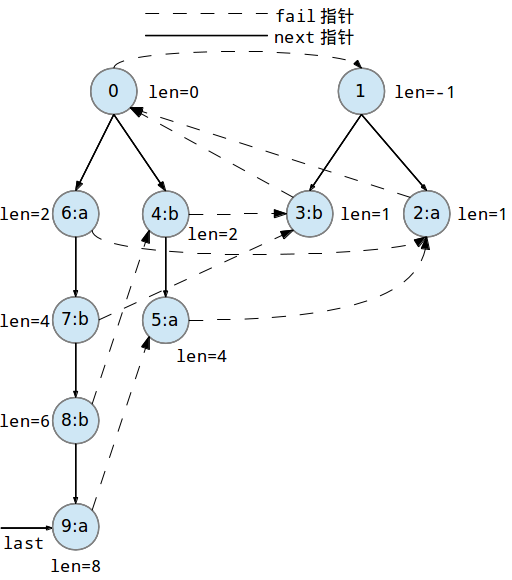
\includegraphics[scale=0.6]{images/Palin.png}
	\label{fig:Palin}
\end{figure}
求串S某个前缀内本质不同回文串的个数、求串S内每一个本质不同回文串出现的次数、求串S内回文串的个数

\begin{lstlisting}[language=C++]
/*
bzoj 3676 [Apio2014]回文串
求出s的所有回文子串中的出现次数乘以长度的最大值。 
*/
#include <cstdio>
#include <cstring>
#include <iostream>
#include <algorithm>
using namespace std;
const int MAXN = 300010 ;
const int N = 26 ;
char s[MAXN];
struct Palindromic_Tree
{
     int next[MAXN][N] ;
     //next指针,next指针和字典树类似,指向的串为当前串两端加上同一个字符构成
     int fail[MAXN] ;//fail指针,失配后跳转到fail指针指向的节点
     int cnt[MAXN] ;
     //节点i表示的回文串在S中出现的次数(建树时求出的不是完全的,count()加上子节点以后才是正确的)
     int num[MAXN] ; // 当前节点通过fail指针到达0节点或1节点的步数(fail指针的深度)
     int len[MAXN] ;//len[i]表示节点i表示的回文串的长度
     int S[MAXN] ;//存放添加的字符
     int last ;//指向上一个字符所在的节点,方便下一次add
     int n ;//字符数组指针
     int p ;//节点指针
     int newnode(int l)     //新建节点
     {
           for(int i = 0 ; i < N ; ++ i) next[p][i] = 0 ;
           cnt[p] = 0 ;
           num[p] = 0 ;
           len[p] = l ;
           return p ++ ;
     }
     void init()   //初始化
     {
           p = 0 ;
           newnode(0) ;
           newnode(-1) ;
           last = 0 ;
           n = 0 ;
           S[n] = -1 ;//开头放一个字符集中没有的字符,减少特判
           fail[0] = 1 ;
     }
     int get_fail(int x)     //和KMP一样,失配后找一个尽量最长的
     {
           while(S[n - len[x] - 1] != S[n]) x = fail[x] ;
           return x ;
     }
     void add(int c,int pos)
     {
           //printf("%d:",p);
           c -= 'a';
           S[++ n] = c ;
           int cur = get_fail(last) ;   //通过上一个回文串找这个回文串的匹配位置
           //printf("%d ",cur);
           if(!next[cur][c]) //如果这个回文串没有出现过,说明出现了一个新的本质不同的回文串
           {
                 int now = newnode(len[cur] + 2) ;   //新建节点
                 fail[now] = next[get_fail(fail[cur])][c] ;   
                 //和AC自动机一样建立fail指针,以便失配后跳转
                 next[cur][c] = now ;
                 num[now] = num[fail[now]] + 1 ;
                 //for(int i=pos-len[now]+1; i<=pos; ++i) printf("%c",s[i]);
           }
           last = next[cur][c] ;
           cnt[last] ++ ;
           //putchar(10);
     }
     void count()
     {
           for(int i = p - 1 ; i >= 0 ; -- i) cnt[fail[i]] += cnt[i] ;
           //父亲累加儿子的cnt,因为如果fail[v]=u,则u一定是v的子回文串!
     }
     long long calc()
     {
         long long ans=0;
         for(int i=2;i<p;i++)
            if(1LL*len[i]*cnt[i]>ans) ans=1LL*len[i]*cnt[i];
         return ans;
     }
} run;
int main()
{
     scanf("%s",s);
     int n=strlen(s);
     run.init();
     for(int i=0; i<n; i++) run.add(s[i],i);
     run.count();
     printf("%lld\n",run.calc());
     return 0;
}
  \end{lstlisting}
每次询问一段区间内的本质不同的回文串个数
\begin{lstlisting}[language=C++]
//https://blog.csdn.net/litble/article/details/80765636
#include<bits/stdc++.h>
using namespace std;
#define RI register int
int read() {
    int q=0;char ch=' ';
    while(ch<'0'||ch>'9') ch=getchar();
    while(ch>='0'&&ch<='9') q=q*10+ch-'0',ch=getchar();
    return q;
}
const int N=100010,M=100010;
struct orzLaofu{//回文树
    int last,n,SZ;
    int a[N][26],fail[N],len[N],s[N],d[N],ff[N];
    //d:等差数列的差值 ff:某一个等差数列开始的那个节点
    void init() {fail[0]=1,len[1]=-1,s[0]=-1,SZ=1;}
    int find(int x,int kn) {
        int js=0;
        while(s[kn-len[x]-1]!=s[kn]) x=fail[x];
        return x;
    }
    void ins(int t) {
        s[++n]=t;int now=find(last,n);
        if(!a[now][t]) {
            fail[++SZ]=a[find(fail[now],n)][t];
            a[now][t]=SZ,len[SZ]=len[now]+2;
            d[SZ]=len[SZ]-len[fail[SZ]];
            ff[SZ]=(d[fail[SZ]]==d[SZ]?ff[fail[SZ]]:SZ);
        }
        last=a[now][t];
    }
    int h[N],ne[N],to[N],in[N],out[N],tot,ti;//建立fail树并获得dfs序
    void add(int x,int y) {to[++tot]=y,ne[tot]=h[x],h[x]=tot;}
    void build_fail_tree() {
        for(RI i=0;i<=SZ;++i) h[i]=-1;
        for(RI i=0;i<=SZ;++i) if(i!=1) add(fail[i],i);
    }
    void dfs(int x) {
        in[x]=++ti;
        for(RI i=h[x];i!=-1;i=ne[i]) dfs(to[i]);
        out[x]=ti;
    }
}T;
int n,m,res;
char s[N];int L[M],ne[M],ans[M],h[N];
struct orzCai{//线段树
    int mx[N<<2];
    void chan(int x,int s,int t,int i,int num) {
        if(s==t) {mx[i]=num;return;}
        int mid=(s+t)>>1;
        if(x<=mid) chan(x,s,mid,i<<1,num);
        else chan(x,mid+1,t,(i<<1)|1,num);
        mx[i]=max(mx[i<<1],mx[(i<<1)|1]);
    }
    int query(int l,int r,int s,int t,int i) {
        if(l<=s&&t<=r) return mx[i];
        int mid=(s+t)>>1,re=0;
        if(l<=mid) re=query(l,r,s,mid,i<<1);
        if(mid+1<=r) re=max(re,query(l,r,mid+1,t,(i<<1)|1));
        return re;
    }
}QvQ;
struct orzBoshi{//树状数组,利用差分实现区间修改单点查询
    int sum[N];
    int lowbit(int x) {return x&(-x);}
    void add(int x,int num) {while(x<=n) sum[x]+=num,x+=lowbit(x);}
    int query(int x) {
        int re=0;
        while(x) re+=sum[x],x-=lowbit(x);
        return re;
    }
}QAQ;
int main()
{
    int k;
    scanf("%s",s+1);
    n=strlen(s+1);
    m=read();
    T.init();
    for(RI i=1;i<=n;++i) T.ins(s[i]-'a');
    T.build_fail_tree(),T.dfs(1);
    for(RI i=1;i<=m;++i)//用链式前向星储存询问
        L[i]=read(),k=read(),ne[i]=h[k],h[k]=i;
    for(RI i=1,x=1;i<=n;++i) {
        x=T.a[T.find(x,i)][s[i]-'a'];
        for(RI j=x;j;j=T.fail[T.ff[j]]) {//在树状数组上搞对答案的影响
            QAQ.add(max(1,QvQ.query(T.in[j],T.out[j],1,T.ti,1)-T.len[j]+2),1);
            QAQ.add(i-T.len[T.ff[j]]+2,-1);
        }
        QvQ.chan(T.in[x],1,T.ti,1,i);
        for(RI j=h[i];j;j=ne[j]) ans[j]=QAQ.query(L[j]);
    }
    for(RI i=1;i<=m;++i)
        printf("%d\n",ans[i]);
    return 0;
}
\end{lstlisting}
\subsection{后缀数组}
\begin{itemize}
	\item 后缀数组sa[i] 字典序第i小的后缀的开头位置
	\item 名次数组rk[i] 保存的是Suffix(i)在所有后缀中从小到大的排名
	\item height数组 定义height[i]=suffix(sa[i-1])和suffix(sa[i])的最长公
	      共前缀,也就是排名相邻的两个后缀的最长公共前缀。
\end{itemize}
\begin{lstlisting}[language=C++]
#define N 200010
int wa[N],wb[N],wv[N],rk[N],c[N],height[N];
int sa[N],a[N];
char s[N];
int cmp(int *r,int a,int b,int l)
{
    return r[a]==r[b] && r[a+l]==r[b+l];
}
void DA(int *r,int *sa,int *rk,int *height,int n,int m)
{
    int i,j,p,*x=wa,*y=wb;
    for(i=0;i<m;i++) c[i]=0;
    for(i=0;i<n;i++) c[x[i]=r[i]]++;
    for(i=1;i<m;i++) c[i]+=c[i-1];
    for(i=n-1;i>=0;i--) sa[--c[x[i]]]=i;
    for(j=1,p=1;p<n;j*=2,m=p)
    {
        for(p=0,i=n-j;i<n;i++) y[p++]=i;
        for(i=0;i<n;i++) if(sa[i]>=j) y[p++]=sa[i]-j;
        for(i=0;i<n;i++) wv[i]=x[y[i]];
        for(i=0;i<m;i++) c[i]=0;
        for(i=0;i<n;i++) c[wv[i]]++;
        for(i=1;i<m;i++) c[i]+=c[i-1];
        for(i=n-1;i>=0;i--) sa[--c[wv[i]]]=y[i];
        swap(x,y);
        for(p=1,x[sa[0]]=0,i=1;i<n;i++)
            x[sa[i]]=cmp(y,sa[i-1],sa[i],j)?p-1:p++;
    }
    int k=0;
    n--;
    for(i=1;i<=n;i++) rk[sa[i]]=i;
    for(i=0;i<n;height[rk[i++]]=k)
        for(k?k--:0,j=sa[rk[i]-1];r[i+k]==r[j+k];k++);
}
\end{lstlisting}

spoj 705 求不同子串的个数
\begin{lstlisting}[language=C++]
int main()
{
    int sk;
    scanf("%d",&sk);
    while(sk--)
    {
        scanf("%s",s);
        int n=strlen(s);
        for(int i=0;i<n;i++) a[i]=s[i];
        a[n++]=0;
        DA(a,sa,rk,height,n,256);
        int ans=0;
        for(int i=0;i<n;i++)
        {
            ans+=n-1-sa[i]-height[i];
            //printf("%d %d\n",i,sa[i]);
        }
        printf("%d\n",ans);
    }
}


  \end{lstlisting}

poj 2774 求两个字符串的最长公共子串
\begin{lstlisting}[language=C++]

int main()
{
    int n,m,len;
    scanf("%s",s);
    n=strlen(s);
    s[n]='#';
    scanf("%s",s+n+1);
    len=strlen(s);
    for(int i=0;i<len;i++) a[i]=s[i];
    a[len++]=0;
    DA(a,sa,rk,height,len,200);
    int ans=0;
    for(int i=1;i<len;i++)
    {
        if((sa[i-1]<n && sa[i]>n) || ((sa[i-1]>n && sa[i]<n)))
           ans=max(ans,height[i]);
    }
    cout<<ans<<endl;
}
  \end{lstlisting}

\subsection{后缀自动机}
\begin{tabularx}{10cm}{llX}  % 10cm 減去前兩個欄位寬度後,剩下的通通給  
	\hline
	Status & Substring                          & endpos          \\
	\hline
	S      &                                    & {0,1,2,3,4,5,6} \\
	1      & a                                  & {1,2,5}         \\
	2      & aa                                 & {2}             \\
	3      & aab                                & {3}             \\
	4      & aabb,abb,bb                        & {4}             \\
	5      & b                                  & {3,4,6}         \\
	6      & aabba,abba,bba,ba                  & {5}             \\
	7      & aabbab,abbab,bbab,bab              & {6}             \\
	8      & ab                                 & {3,6}           \\
	9      & aabbabd,abbabd,bbabd,babd,abd,bd,d & {7}             \\
	\hline\label{key}
\end{tabularx}

\begin{figure}[h!]
	\centering
	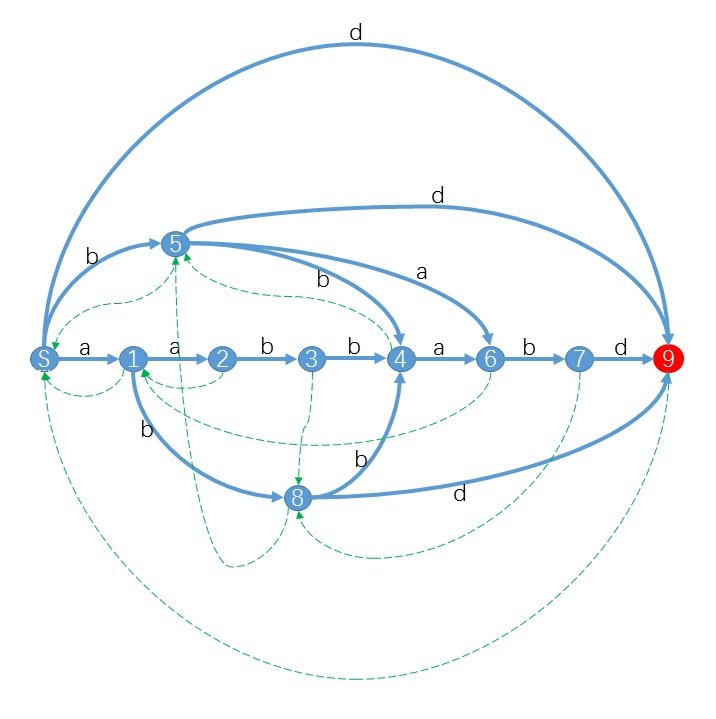
\includegraphics[scale=0.8]{images/sam.jpg}
	\label{fig:sam}
\end{figure}

\begin{itemize}
	\item 对于一个字符串S,它对应的后缀自动机是一个最小的确定有限状态自动机,接受且只接受S的后缀。
	\item S的子串最终会到达一个合法状态,不是子串的话最终会无路可走。
	\item 对于S的两个子串$s1$和$s2$,不妨设$length(s1) \leq length(s2)$,$s1$是$s2$的后缀当且仅当$endpos(s2) \subseteq endpos(s1)$,$s1$不是$s2$的后缀当且仅当$endpos(s1) \bigcap endpos(s2) = \emptyset$
	\item 对于一个状态$st$,以及任意$s \in substrings(st)$,都有$s$是$longest(st)$的后缀。
	\item 对于一个状态$st$,以及任意的$longest(st)$的后缀$s$,如果$s$的长度满足:$length(shortest(st)) \leq length(s) \leq length(longest(st))$,那么$s \in substrings(st)$
	\item 广义后缀自动机,比如多个串,每个串插入前让last=1,或者对一个trie树建广义后缀自动机,添加每个点以父节点的last继承过来,类似树上主席树insert的方式。加上最后一段的while的复杂度据说是带一个根号的。
	\item 维护什么东西的时候拓扑排序转移一下总不会错!
\end{itemize}


\begin{lstlisting}[language=C++]
#include<bits/stdc++.h>
using namespace std;
typedef long long ll;
#define N 100010
struct SAM
{
    int tot,last;
    int son[N<<1][26],maxlen[N<<1],pre[N<<1];
    int in[N<<1],q[N<<1],cnt[N<<1],v[N<<1];
    int ans[N<<1];
    int lc[N<<1],strval[N<<1];
    ll sum[N<<1];
    void init()//记得初始化
    {
        tot=0;
        last=newnode();
    }
    int newnode()
    {
        ++tot;
        memset(son[tot],0,sizeof(son[tot]));
        maxlen[tot]=pre[tot]=in[tot]=cnt[tot]=0;
        return tot;
    }
    void add(int id,int c)//id表示串的编号,一定要从1开始
    {
        int now=newnode();
        maxlen[now]=maxlen[last]+1;
        cnt[now]=1;
        while(last && son[last][c]==0)
            son[last][c]=now,last=pre[last];
        if(last)
        {
            int x=son[last][c];
            if(maxlen[x]==maxlen[last]+1) pre[now]=x;
            else
            {
                int nq=newnode();
                maxlen[nq]=maxlen[last]+1;
                memcpy(son[nq],son[x],sizeof(son[x]));
                pre[nq]=pre[x];
                lc[nq]=lc[x];strval[nq]=strval[x];
                pre[x]=pre[now]=nq;
                while(last && son[last][c]==x)
                    son[last][c]=nq,last=pre[last];
            }
        }
        else pre[now]=1;
        last=now;
        //广义sam
        while(now && lc[now]!=id)
        {
            lc[now]=id;
            mulmod(strval[now],val[id]);//给状态now加上第id个串的信息
            now=pre[now];
        }
    }
    //求不同子串个数
    ll count()
    {
        ll ans=0;
        for(int i=1;i<=tot;++i)
            ans+=maxlen[i]-maxlen[pre[i]];
        return ans;
    }
    //求恰好出现k次的不同子串的个数
    ll count(int k)
    {
        calc();
        ll ans=0;
        for(int i=1;i<=tot;++i)
            if(cnt[i]==k)
                ans+=maxlen[i]-maxlen[pre[i]];
        return ans;
    }
    //拓扑排序求endpos集合大小
    void calc()
    {
        int l=0,r=0;
        for(int i=1;i<=tot;++i) ++in[pre[i]];
        for(int i=1;i<=tot;++i)
            if(!in[i])
                q[r++]=i;
        while(l!=r)
        {
            int x=q[l++];
            if(pre[x]==0) continue;
            cnt[pre[x]]+=cnt[x];
            if((--in[pre[x]])==0)
                q[r++]=pre[x];
        }
    }
    //也可以对maxlen从大到小排序,opt为true表示不同位置的相同子串算作多个
    //广义sam这么写可能有问题?
    void calc(bool opt)
    {
        for(int i=1;i<=tot;++i) v[maxlen[i]]++;
        for(int i=1;i<=tot;++i) v[i]+=v[i-1];
        for(int i=tot;i;i--) q[v[maxlen[i]]--]=i;
        for(int i=tot;i;i--)
        {
            int x=q[i];
            if(opt) cnt[pre[x]]+=cnt[x];
            else cnt[x]=1;
        }
        cnt[1]=0;
        for(int i=tot;i;i--)
        {
            int x=q[i];
            sum[x]=cnt[x];
            for(int j=0;j<26;++j)
                sum[x]+=sum[son[x][j]];
        }
    }
    //求第k小子串,需调用calc(bool opt)
	void dfs(int x,ll k)
    {
        if(k<=cnt[x]) return;
        k-=cnt[x];
        for(int i=0;i<26;++i)
        if(son[x][i])
        {
            if(k<=sum[son[x][i]])
            {
                putchar(i+'a');
                dfs(son[x][i],k);
                return;
            }
            else k-=sum[son[x][i]];
        }
    }    
    //求长度为i的子串中出现次数最多的出现次数
    void solve(int len)
    {
        calc();
        for(int i=1;i<=tot;++i)
            if(ans[maxlen[i]]<cnt[i])
                ans[maxlen[i]]=cnt[i];
        for(int i=len-1;i>=1;--i)
            if(ans[i]<ans[i+1])
                ans[i]=ans[i+1];
        for(int i=1;i<=len;i++)
            printf("%d\n",ans[i]);
    }
    //求最长公共子串的长度
    int ask(char *s)
    {
        int now=1,len=0,ans=0;
        for(int i=0;s[i];++i)
        {
            int x=s[i]-'a';
            if(son[now][x])
            {
                now=son[now][x];
                ++len;
            }
            else
            {
                while(now && son[now][x]==0)
                    now=pre[now];
                if(now==0) now=1,len=0;
                else len=maxlen[now]+1,now=son[now][x];
            }
            ans=max(ans,len);
        }
        return ans;
    }
	void debug()
    {
        for(int i=1;i<=tot;++i)
        {
            cout<<i<<" : ";
            for(int j=0;j<26;++j)
            if(son[i][j])
                cout<<(char)(j+'a')<<"->"<<son[i][j]<<" ";
            cout<<"== pre->"<<pre[i]<<" == cnt->"<<cnt[i]<<endl;
        }
    }
} sam;

int main()
{
    sam.init();//!!!
    sam.add(s[i]-'a');
}

  \end{lstlisting}


\subsection{正则表达式}
\begin{itemize}
	\item ``.''匹配除``\textbackslash n''之外的任何单个字符。
	\item ``\textbackslash \^\quad ''匹配输入字符串的开始位置,``\textbackslash \$''匹配输入字符串结尾的位置。
	\item ``|'' 两个匹配条件逻辑或。
	\item ``\textbackslash w''匹配字母或数字或下划线,``\textbackslash W''匹配任意不是字母、数字、下划线的字符。
	\item ``\textbackslash d''匹配任意一个数字,``\textbackslash D''匹配任意非数字字符。

	\item ``*''0次或多次匹配前面的字符或子表达式,``+''1次或多次匹配前面的字符或子表达式,``?''0次或1次匹配前面的字符或子表达式。
	\item ``\{n\}'' 正好匹配n次。``\{n,\}'' 至少匹配n次。``\{n,m\}'' 匹配n到m次。
	\item ``[xyz]''字符集,匹配包含的任一字符。
	\item ``\textbackslash b''匹配一个单词边界,``\textbackslash B''匹配非单词边界。
\end{itemize}

\begin{lstlisting}[language=C++]
/*
hdu 6170
str1 包含大小写字母
str2 包含.*,但是题中的.*是重复匹配单个字符比如aaaa,bb,这里需要用分组与捕获
*/
#include<bits/stdc++.h>
using namespace std;
string str1,str2;
int main()
{
    int T;
    scanf("%d",&T);
    while(T--)
    {
        cin>>str1>>str2;
        regex reg_rep("\\.\\*");
        str2=regex_replace(str2,reg_rep,"(\\w)\\1*");
        regex reg(str2);
        if(regex_match(str1,reg)) puts("yes");
        else puts("no");
    }
}

\end{lstlisting}

\begin{lstlisting}[language=C++]
/*

缩写单词
*/
#include<bits/stdc++.h>
using namespace std;
int main()
{
    freopen("abbreviation.in","r",stdin);
    freopen("abbreviation.out","w",stdout);
    regex reg("\\b([A-Z][a-z]+ )+([A-Z][a-z]+)\\b");
    smatch reg_match;
    string str;
    while(getline(cin,str))
    {
        int len=str.length();
        while(regex_search(str,reg_match,reg))
        {
            string sub=reg_match[0];
            int sublen=sub.length();
            int pos=str.find(sub);
            for(int i=0;i<pos;++i) putchar(str[i]);
            for(int i=0;i<sublen;++i)
            if(isupper(sub[i]))
                putchar(sub[i]);
            putchar(' ');
            putchar('(');
            for(int i=0;i<sublen;++i) putchar(sub[i]);
            putchar(')');
            str=reg_match.suffix().str();
        }
        for(auto &ch:str) putchar(ch);
        puts("");
    }
}

\end{lstlisting}
\section{数学}
\subsection{Formula}
\subsubsection*{组合数}
$C_r^{k}=\frac{r}{k}C_{r-1}^{k-1}$\qquad
$C_r^{k}=C_{r-1}^{k}+C_{r-1}^{k-1}$\qquad
$C_r^mC_m^k=C_r^kC_{r-k}^{m-k}$\par
$\sum_{k \le n}C_{r+k}^k=C_{r+n+1}^{n}$\qquad
$\sum_{0 \le k \le n}C_{k}^{m}=C_{n+1}^{m+1}$\par
$\sum_{0 \le i \le n}C_n^{i}=2^n$\qquad
$\sum_{0 \le i \le n}C_n^{i}\times i =n\times 2^{n-1}$\qquad
$\sum_{0 \le i \le n}C_n^{i}\times i^2 =n\times(n+1)\times  2^{n-2}$\par
$\sum_{0 \le i \le n}(C_n^{i})^2=C_{2n}^{n}$\par
The number of non-negative solutions to equation\par  $x_1+x_2+x_3+\dots+x_k=n$ is $\tbinom{n+k-1}{k-1}$\par
$x_1+x_2+x_3+\dots+x_k=n (0\le x_i\le S)$is  $\sum_{i=0}^{k}(-1)^i\tbinom{k}{i}\tbinom{n+k-1-i(S+1)}{k-1}$
\subsubsection*{威尔逊定理}
$(p-1)!\equiv -1\pmod{p}$
\subsubsection*{Catalan number}
$C_n=\frac{1}{n+1}\tbinom{2n}{n}$\qquad
$C_n=\frac{4n-2}{n+1}C_{n-1}=C(2n,n)-C(2n,n-1)$

\subsubsection*{Burnside’s Lemma}
$\left|X/G\right|=\frac{1}{\left|G\right|}\sum_{g \in G}\left|X^g\right|$

$Polya: X^g=t^{c(g)}$

Let $X^g$ denote the set of elements in $X$ fixed by $g$.
$c(g)$ is the number of cycles of the group element $g$ as a permutation of $X$.

\subsubsection*{第一类Stirling数}
n个元素划分成k个圆排列的方案数

$s(n,k)=s(n-1,k-1)+s(n-1,k)\times(n-1)$

记$x$的$n$次上升幂为 $x^{\overline{n}}$

$x^{\overline{n}}=\prod_{i=0}^{n-1}(x+i)=\sum_{i=0}^{n-1}s(n,i)x^i$

\subsubsection*{第二类Stirling数}
n个元素划分成k个集合的方案数

$S(n,k)=S(n-1,k-1)+S(n-1,k) \times k$

\subsubsection*{降幂公式}
$a^b\%p=a^{(b\%\varphi(p))+\varphi(p)}\%p(b\geq\varphi(p))$
\subsubsection*{错位排列}
$0,1,2,9,44,265,1854,14833,133496,41334961$

$D_n=n!(1-\frac{1}{1!}+\frac{1}{2!}+\dots+(-1)^n\frac{1}{n!})=\left\lfloor {\frac  {n!}{e}}+0.5\right\rfloor$

$D_n=n\times D_{n-1}+(-1)^n$,$D_n=(n-1)\times(D_{n-1}+D_{n-2})$

\subsubsection*{Bell数}
$B_n$表示把$n$个带标号的物品划分为若干不相交集合的方案数。\par
$B_{n+1}=\sum_{k=0}^nC(n,k)B_k$\par
$B_{n}=\sum_{k=1}^nS(n,k)$\par
\subsubsection*{蔡勒公式}
\begin{lstlisting}[language=C++] 
int calc(int day,int month,int year)
{
    if(!isleap(year) && month==2 && day==29) return -1;
    if(month<=2) year--,month+=12;
    return ((1LL*day+2LL*month+3LL*(month+1)/5+1LL*year+1LL*year/4-year/100+year/400)%7+7)%7;
}  
\end{lstlisting}


\subsubsection*{皮克定理}
适用于顶点坐标都是整点的简单多边形。面积$A$,内部格点数目$i$,边上格点数目$b$的关系 \par
$A=i+b/2-1$

\subsubsection*{幻方构造}
\begin{lstlisting}[language=C++]
int n;
int a[50][50];
int main()
{
    scanf("%d",&n);
    int x=1,y=(n+1)/2;
    a[x][y]=1;
    for(int i=2;i<=n*n;i++)
    {
        if(x==1 && y!=n) x=n,y++;
        else if(x!=1 && y==n) x--,y=1;
        else if(x==1 && y==n) x++;
        else if(!a[x-1][y+1]) x--,y++;
        else x++;
        a[x][y]=i;
    }
    for(int i=1;i<=n;i++)
        for(int j=1;j<=n;j++)
            printf("%d%c",a[i][j],(j<n)?' ':'\n');
}
        \end{lstlisting}
\subsubsection*{勾股数完全公式}
\begin{itemize}
	\item 公式$a=m,b=\frac{m^2/k-k}{2},c=\frac{m^2/k+k}{2}$
	\item 当m确定为任意一个大于等于3的奇数时,k={1,m\^2的所有小于m的因子}
	\item 当m确定为任意一个大于等于4的偶数时,k={m\^2 / 2的所有小于m的偶数因子}
\end{itemize}
\begin{lstlisting}[language=C++]   
/*Codeforces Round #368 (Div. 2) C Pythagorean Triples */
    long long n;
    cin>>n;
    if(n<3) puts("-1");
    else
    {
        if(n&1)cout<<(n*n-1)/2<<" "<<(n*n+1)/2<<endl;
        else cout<<(n*n/2-2)/2<<" "<<(n*n/2+2)/2<<endl;
    }
        \end{lstlisting}
\subsubsection*{固定k个点为根的带标号有根树森林计数}
固定$k$个点作为根的$n$个点的带标号有根树森林的方案数是$k\times n^{n-k-1}$。
\subsubsection*{斯特林近似公式}
$n!\approx\sqrt{2\pi n}(\frac{n}{e})^n$

\subsubsection*{maxmum-minmum identity}
\begin{equation}
	\begin{aligned}
		\max\{x_{1},x_{2},\ldots ,x_{{n}}\} & =\sum _{{i=1}}^{n}x_{i}-\sum _{{i<j}}\min\{x_{i},x_{j}\}+\sum _{{i<j<k}}\min\{x_{i},x_{j},x_{k}\}-\cdots \\&\qquad \cdots +\left(-1\right)^{{n+1}}\min\{x_{1},x_{2},\ldots ,x_{n}\},
	\end{aligned}
\end{equation}
\subsubsection*{生成树计数}
有标号,完全图,无根树:Cayley's Formula,$T_n=n^{n-2}$
有标号,完全图,k选定根,生成森林,$T_{n,k}=k^2n^{n-k-1}$
\subsubsection*{环}
有标号,无孤立点,有向:错位排列 $dp_{n}=(n-1)(dp_{n-1}+dp_{n-2})$
有标号,无孤立点,无向	$dp_{n}=(n-1)(dp_{n-1}+dp_{n-2})-\frac{(n-1)(n-2)}{2}dp_{n-3}$
\subsection{prufer编码}
对于一棵树,我们每次将编号最小的叶子节点的父亲放到序列中,并将该叶子节点删除掉,如此操作一直到只剩两个节点为止,那么此时我们就得到了一棵树的有n-2项的prufer编码,显然,每一个合法的prufer编码与树是一一对应的。现在我们可以把一些有关树的信息与其对应的prufer编码相关联,某一节点的度数等于该节点编号在prufer编码里面的出现次数+1(他的每一个儿子必然都会在序列里面将他生成一次,而他还有一个父亲),现在通过prufer编码我们可以解决一类关于给定度数条件的树计数问题。
对于当前给定的度数条件我们可以翻译为他在prufer编码里面出现了多少次,对于这个次数我们可以通过全排列再除以交换相同项的方式来得到最后的答案。
\subsection{矩阵乘法}
\begin{lstlisting}[language=C++]
//正常版本:无需担心RE
int c[N][N];
void MUL(int a[][N],int b[][N],int d[][N],int n,int m,int p)
{
	memset(c,0,sizeof(c));
	rep(i,0,n-1)rep(k,0,m-1)if(a[i][k])rep(j,0,p-1)
	{	
		up(c[i][j],1ll*a[i][k]*b[k][j]%mod);
	}
	rep(i,0,n-1)rep(j,0,p-1)d[i][j]=c[i][j];
}
//矩阵乘法快速幂:记录当前位置l,目标位置r,转移次数r-l,考虑从l位置开始递推下一项需要乘上的矩阵

//优化取模版本
const ll mod2=(ll)mod*mod;
void up(ll &a,ll b,ll mod){
	a+=b;
	if(a>=mod)a-=mod;
}
void MUL(int a[][N],int b[][N],int d[][N],int n){
	memset(c,0,sizeof(c));
	rep(i,0,n-1)rep(j,0,n-1){
		ll tmp=0;
		rep(k,0,n-1)up(tmp,(ll)a[i][k]*b[k][j],mod2);
		c[i][j]=tmp%mod;
	}
	rep(i,0,n-1)rep(j,0,n-1)d[i][j]=c[i][j];
}
\end{lstlisting}

\subsection{Bernoulli数}
\begin{itemize}
	\item $S_m(n)=\sum_{k=1}^{n}k^m$
	\item $S_m(n)$显然是一个$m+1$阶多项式,用伯努利数显式地写出该多项式。
	\item $S_m(n)= \frac{1}{m+1} \sum_{k=0}^{m} \dbinom{m+1}{k}B_{k}^{+}n^{m+1-k}$
	\item 这里$B_{k}^{+}$表示第二类伯努利数,$B_1^+=+\frac{1}{2}$
\end{itemize}

$O(nlogn)$求Bernoulli数

$\frac{x}{e^x-1}=\sum_{n=0}^{\inf}B_n^-\frac{x^n}{n!}$
根据伯努利数指数型母函数,通过对分母泰勒展开,将求伯努利数的问题归结到多项式求逆的问题.

需要特别注意的是这里求出的是第一类伯努利数,需要对$B_1$取相反数得到第二类伯努利数.

\begin{lstlisting}[language=C++] 
void Bernoulli(){
    fac[0]=ifac[0]=inv[0]=1;
    fac[1]=ifac[1]=inv[1]=1;
    rep(i,2,maxn){
        fac[i]=(ll)fac[i-1]*i%mod;
        inv[i]=(mod-mod/i)*(ll)inv[mod%i]%mod;
        ifac[i]=ifac[i-1]*(ll)inv[i]%mod;
    }
    rep(i,0,maxn-1)a[i]=ifac[i+1];
    int len=1<<17;
    NTT::init();
    get_inv(a,b,len);
    rep(i,0,len-1)b[i]=b[i]*(ll)fac[i]%mod;
    b[1]=mod-b[1];
}
\end{lstlisting}

\subsection{高维前缀和}
求超集和
\begin{lstlisting}[language=C++] 
void doit(int *f,int n)
{
    int len=1<<n;
    for(int i=0;i<n;++i)
        for(int j=0;j<len;++j)
            if(~j&(1<<i))
                f[j]+=f[j^(1<<i)];
}
\end{lstlisting}

dfs出now的所有约数($10^6$级别),求每种约数分别是多少个数的约数。
写法十分精妙。
\begin{lstlisting}[language=C++] 
void work(ll now)
{
    cnt=len=0;
    divide(now);
    dfs(1,1);
    sort(dv+1,dv+len+1);
    for(int i=1;i<=len;++i) f[i]=0;
    for(int i=1;i<=n;++i)
    {
        ll g=__gcd(now,a[i]);
        ++f[lower_bound(dv+1,dv+len+1,g)-dv];
    }
    for(int i=1;i<=cnt;++i)
    {
        ll x=p[i];
        for(int j=len,k=len;j>=1;--j)
        if(dv[j]%x==0)
        {
            ll y=dv[j]/x;
            while(dv[k]>y) --k;
            f[k]+=f[j];
        }
    }
    for(int i=1;i<=len;++i)
        if(f[i]>=n-k)
            ans=max(ans,dv[i]);
}
\end{lstlisting}
\subsection{多项式插值}
\begin{itemize}
	\item 模数为质数
	\item 对多项式求和:求和后为d+1阶多项式,利用calcn计算相关项
	\item calcn    : a[0].....a[d+1] a[n]
	\item qpolysum : a[0].....a[d+1] $\sum_{i=0}^{n-1} a[i]*R^i$
\end{itemize}
\begin{lstlisting}[language=C++] 
namespace polysum
{
    const int D=101000;
    LL a[D],f[D],g[D],p[D],p1[D],p2[D],b[D],h[D][2],C[D];
    LL calcn(int d,LL *a,LL n)
    {
        if(n<=d)return a[n];
        p1[0]=p2[0]=1;
        rep(i,0,d)
        {
            LL t=(n-i+mod)%mod;
            p1[i+1]=p1[i]*t%mod;
        }
        rep(i,0,d)
        {
            LL t=(n-d+i+mod)%mod;
            p2[i+1]=p2[i]*t%mod;
        }
        LL ans=0;
        rep(i,0,d)
        {
            LL t=g[i]*g[d-i]%mod*p1[i]%mod*p2[d-i]%mod*a[i]%mod;
            if((d-i)&1)ans=(ans-t+mod)%mod;
            else ans=(ans+t)%mod;
        }
        return ans;
    }
    void init(int M)
    {
        f[0]=f[1]=g[0]=g[1]=1;
        rep(i,2,M+4)f[i]=f[i-1]*i%mod;
        g[M+4]=qpow(f[M+4],mod-2);
        dow(i,M+3,1)g[i]=g[i+1]*(i+1)%mod;
    }
    LL polysum(LL n,LL *a,LL m)
    {
        a[m+1]=calcn(m,a,m+1);
        rep(i,1,m+1) a[i]=(a[i-1]+a[i])%mod;
        return calcn(m+1,a,n-1);
    }
    LL qpolysum(LL R,LL n,LL *a,LL m)
    {
        if (R==1) return polysum(n,a,m);
        a[m+1]=calcn(m,a,m+1);
        LL r=qpow(R,mod-2),p3=0,p4=0,c,ans;
        h[0][0]=0;h[0][1]=1;
        rep(i,1,m+1)
        {
            h[i][0]=(h[i-1][0]+a[i-1])*r%mod;
            h[i][1]=h[i-1][1]*r%mod;
        }
        rep(i,0,m+1)
        {
            LL t=g[i]*g[m+1-i]%mod;
            if (i&1) p3=((p3-h[i][0]*t)%mod+mod)%mod,p4=((p4-h[i][1]*t)%mod+mod)%mod;
            else p3=(p3+h[i][0]*t)%mod,p4=(p4+h[i][1]*t)%mod;
        }
        c=qpow(p4,mod-2)*(mod-p3)%mod;
        rep(i,0,m+1) h[i][0]=(h[i][0]+h[i][1]*c)%mod;
        rep(i,0,m+1) C[i]=h[i][0];
        ans=(calcn(m,C,n)*qpow(R,n)-c)%mod;
        if (ans<0) ans+=mod;
        return ans;
    }
}
\end{lstlisting}
\subsection{多项式inv,ln,exp:NTT实现}
\begin{itemize}
	\item 多项式存在a[0]......a[t-1]
	\item 多项式的inv,ln,exp存在b[0]......b[t-1]
	\item 原多项式放在a[0]......b[t-1]
	\item 多项式对$x^t$取模
	\item 注意数组大小,注意预处理长度,注意将多项式长度操作为2的整数次幂
\end{itemize}
\begin{lstlisting}[language=C++]
#include <bits/stdc++.h>
#define rep(i,s,t) for(int i = s;i <= t;i ++)
#define dow(i,t,s) for(int i = t;i >= s;i --)
#define REP(i,x) for(int i = 0;i < x.size();i ++)
#define DOW(i,x) for(int i = (int)s.size();i >= 0;i --)

#define fi first
#define se second

#define pb push_back
#define mp make_pair
#define lb lower_bound
#define ub upper_bound

#define eps 1e-6
#define INF
#define NN 150010
#define SZ(x) ((int)(x).size())

using namespace std;
const int mod=998244353;
const int maxn=550010;

typedef vector<int> VI;
typedef long long ll;;
typedef double db;
typedef pair<int,int> PII;

int qpow(int a,int b){
	int ret=1;
	while(b){
		if(b&1)ret=(ll)ret*a%mod;
		a=(ll)a*a%mod;
		b>>=1;
	}
	return ret;
}
int f[NN<<2],g[NN<<2],h[NN<<2],sf[NN<<2],sg[NN<<2],sh[NN<<2],tmp[NN<<2],tmp2[NN<<2];
int inv[NN<<2];

namespace NTT{
    const int g=3;


    int x[NN<<2],y[NN<<2],wn[NN<<2];
    void init()
    {
        rep(i,0,20)wn[i]=qpow(g,(mod-1)/(1<<i));
    }

    void brc(int *F,int len)
    {
        int j=len/2;
        rep(i,1,len-2){
            if(i<j)swap(F[i],F[j]);
            int k=len/2;
            while(j>=k) j-=k,k>>=1;
            if(j<k)j+=k;
        }
    }

    void NTT(int *F,int len,int t)
    {
        int id=0; brc(F,len);
        for(int h=2;h<=len;h<<=1)
        {
            id++;
            for(int j=0;j<len;j+=h)
            {
                int E=1;
                for(int k=j;k<j+h/2;k++)
                {
                    int u=F[k],v=(ll)E*F[k+h/2]%mod;
                    F[k]=(u+v)%mod,F[k+h/2]=((u-v)%mod+mod)%mod;
                    E=(ll)E*wn[id]%mod;
                }
            }
        }
        if(t==-1)
        {
            rep(i,1,len/2-1)swap(F[i],F[len-i]);
            ll inv=qpow(len,mod-2);
            rep(i,0,len-1)F[i]=(ll)F[i]%mod*inv%mod;
        }
    }
    void multiply(int *a,int len1,int *b,int len2)
    {
        int len=1;
        while(len<len1+len2)len<<=1;
        rep(i,len1,len-1)a[i]=0;
        rep(i,len2,len-1)b[i]=0;
        NTT(a,len,1); NTT(b,len,1);
        rep(i,0,len-1)a[i]=(ll)a[i]*b[i]%mod;
        NTT(a,len,-1);
    }
}
inline void getinv(int *a,int *b,int n){
	if(n==1){b[0]=qpow(a[0],mod-2);return;}

	getinv(a,b,n>>1);
	int k=n<<1;
	rep(i,0,n-1)tmp[i]=a[i];
	rep(i,n,k-1)tmp[i]=b[i]=0;
	NTT::NTT(tmp,k,1),NTT::NTT(b,k,1);
	rep(i,0,k-1){
		b[i]=(ll)b[i]*(2-(ll)tmp[i]*b[i]%mod)%mod;
		if(b[i]<0)b[i]+=mod;
	}
	NTT::NTT(b,k,-1);
	rep(i,n,k-1)b[i]=0;
}
inline void getln(int *a,int *b,int n){
	getinv(a,tmp2,n);
	int k=n<<1;
	rep(i,0,n-2)b[i]=(ll)a[i+1]*(i+1)%mod;
	rep(i,n-1,k-1)b[i]=0;
	NTT::NTT(b,k,1),NTT::NTT(tmp2,k,1);
	rep(i,0,k-1)b[i]=(ll)b[i]*tmp2[i]%mod;
	NTT::NTT(b,k,-1);
	dow(i,n-1,0)b[i]=(ll)b[i-1]*inv[i]%mod;b[0]=0;
}
inline void getexp(int *a,int *b,int n){
	if(n==1){b[0]=1;return ;}
	getexp(a,b,n>>1);
	getln(b,tmp,n);
	int k=n<<1;
	rep(i,0,n-1){
		tmp[i]=a[i]-tmp[i];
		if(tmp[i]<0)tmp[i]+=mod;
	}
	if((++tmp[0])==mod)tmp[0]=0;
	rep(i,n,k-1)tmp[i]=b[i]=0;
	NTT::NTT(tmp,k,1),NTT::NTT(b,k,1);
	rep(i,0,k-1)b[i]=(ll)b[i]*tmp[i]%mod;
	NTT::NTT(b,k,-1);
	rep(i,n,k-1)b[i]=0;
}

void init(){
	inv[0]=inv[1]=1;
	rep(i,2,maxn)inv[i]=(mod-mod/i)*(ll)inv[mod%i]%mod;
	int len=1<<17;
	NTT::init();
}
int main ()
{
	#ifdef Faraway
    freopen("in.in","r",stdin);
    freopen("out.out","w",stdout);
    #endif
    init();
    int n,m,k;
    scanf("%d%d%d",&n,&m,&k);
    rep(i,0,n)scanf("%d",f+i);
    rep(i,0,m)scanf("%d",g+i);

    int len=1;
    while(len<k*2+10)len<<=1;

    getln(f,sf,len);
    getln(g,sg,len);
    h[0]=0;
    rep(i,1,len-1)sh[i]=(ll)i*sf[i]%mod*sg[i]%mod;
    for(int i=0;i<len;i+=2)sh[i]=(mod-sh[i])%mod;
    getexp(sh,h,len);
    rep(i,0,k-1)printf("%d%c",h[i],i==k-1?'\n':' ');
    return 0;
}

\end{lstlisting}

\subsection{二次剩余}
求解方程: $x^2\equiv n\pmod{p}$,无解返回$-1$, 否则返回其中一个解$r$, 另一个解是$p-r$。\par
\begin{lstlisting}[language=C]
LL ToneLLi_Shanks(LL n, LL p) {
  if (p == 2) return (n & 1) ? 1 : -1;
  if (pow_mod(n, p >> 1, p) != 1) return -1;
  if (p & 2) return pow_mod(n, p + 1 >> 2, p);
  int s = __builtin_ctzll(p ^ 1);
  LL q = p >> s, z = 2;
  for (; pow_mod(z, p >> 1, p) == 1; ++z);
  LL c = pow_mod(z, q, p);
  LL r = pow_mod(n, q + 1 >> 1, p);
  LL t = pow_mod(n, q, p), tmp;
  for (int m = s, i; t != 1;) {
    for(i=0,tmp=t;tmp!=1;++i)tmp=tmp*tmp%p;
    for (; i < --m;) c = c * c % p;
    r=r*c%p;c=c*c%p;t=t*c%p;}
  return r;}
\end{lstlisting}

\subsection{数论公式}
对任意$i,j,(i,m)=(j,m),(x,m)=0,i*x^k1=i,j*x^k2=j$,有$k1=k2$,(其中k1,k2是最小循环节)\par
若$x^p=1$,要找最小循环节,只需要独立枚举p的每种素数的指数。\par

常见积性函数:\par
$id(n)=n$\qquad
$e(n)=[n=1]$\qquad
$I(n)=1$\par
$d(n)=\sum_{d|n}1$\qquad
$\sigma(n)=\sum_{d|n}d$\par
欧拉函数$\varphi(n)$\qquad
莫比乌斯函数$\mu(n)$\par
一些性质:\par
$n=\sum_{d|n}\varphi(d)$\qquad($id=\varphi \times I$)\par
$e(n)=\sum_{d|n}\mu(d)$\qquad($e=\mu \times I$)\par
$\mu\times id=\varphi$\par
$\sum_{i=1}^n\sum_{j=1}^m i\times j[\gcd(i,j)=d]=\sum_{i=1}^{\lfloor\frac{n}{d}\rfloor}\sum_{j=1}^{\lfloor\frac{m}{d}\rfloor} id\times jd[\gcd(i,j)=1]$\par
$\mu^2(n)=\sum_{d^2|n}\mu(d)$\par
$\sum_{i=1}^nd(n)=\sum_{i=1}^n\lfloor\frac{n}{i}\rfloor$\par
莫比乌斯反演:\par
$f(n)=\sum_{d|n}g(d)$\par
$g(n)=\sum_{d|n}\mu(d)f(\frac{n}{d})$\par
$f(n)=\sum_{i=1}^nt(i)g(\lfloor\frac{n}{i}\rfloor)$\par
$g(n)=\sum_{i=1}^n\mu(i)t(i)f(\lfloor\frac{n}{i}\rfloor)$\par
杜教筛:\par
\begin{itemize}
	\item 记$S(n)=\sum_{i=1}^{n}f(i)$,设法找到一个$g(x)$,得到递推式$g(1)S(n)=\sum_{i=1}^{n}(f\times g)(i)-\sum_{i=2}^{n}g(i)S(\lfloor\frac{n}{i}\rfloor)$
	\item 求$S(n)=\sum_{i=1}^n (f \cdot g)(i)$的值且$g(x)$为完全积性函数,这时有$S(n)=\sum_{i=1}^n[(f\times 1) \cdot g](i)-\sum_{i=2}^n S(\lfloor \frac{n}{i} \rfloor)g(i)$
	\item 求$S(n)=\sum_{i=1}^n (f\times g)(i)$的值,这时有
	      $S(n)=\sum_{i=1}^n g(i)\sum_{ij \leq n}(f\times 1)(j)-\sum_{i=2}^n S(\lfloor \frac{n}{i} \rfloor)$
\end{itemize}


\subsection{莫比乌斯函数}
\begin{itemize}
	\item 作为容斥系数求1到n中有多少不含完全平方数因子的数
\end{itemize}
\begin{lstlisting}[language=C++]
ll calc(ll n)
{
    ll ans=0;
    for(int i=1;i<=n/i;i++)
        ans+=mu[i]*n/(1LL*i*i);
    return ans;
}
\end{lstlisting}

\subsection{杜教筛}
求$\sum_{d=1}^{m}\mu(d)\times {\left\lfloor m/d \right\rfloor}^n$,模$2^{64}$
\begin{lstlisting}[language=C++]
#include<bits/stdc++.h>
using namespace std;
typedef unsigned long long ull;
typedef long long ll;
#define rep(i,l,r) for(int i=l;i<=r;++i)
const int N=20000000;
int prime[N],tot;
bool vis[N+5];
int mu[N+5],S[N+5];
ll n,m;
unordered_map<ll,ull> mp;
ull power(ull x,ll n)
{
    ull ans=1;
    while(n)
    {
        if(n&1) ans=ans*x;
        x=x*x;
        n>>=1;
    }
    return ans;
}
void getprime()
{
    mu[1]=1;
    for(int i=2; i<=N; ++i)
    {
        if(!vis[i])
        {
            prime[tot++]=i;
            mu[i]=-1;
        }
        for(int j=0; j<tot && prime[j]<=N/i; ++j)
        {
            vis[i*prime[j]]=true;
            if(i%prime[j]==0)
            {
                mu[i*prime[j]]=0;
                break;
            }
            else mu[i*prime[j]]=-mu[i];
        }
    }
    for(int i=1; i<=N; ++i) S[i]=S[i-1]+mu[i];
}
ull calc(ll n)
{
    if(n<=N) return S[n];
    if(mp.count(n)) return mp[n];
    ull ans=1;
    for(ll l=2,r; l<=n; l=r+1)
    {
        r=n/(n/l);
        ans-=calc(n/l)*(r-l+1);
    }
    return mp[n]=ans;
}
int main()
{
    getprime();
    while(cin>>n>>m)
    {
        swap(n,m);
        ull ans=0,pre=0;
        for(ll d=1; d<=n; ++d)
        {
            ull now=calc(n/(n/d));
            ans+=power(n/d,m)*(now-pre);
            d=(n/(n/d));
            pre=now;
        }
        cout<<ans<<endl;
    }
}

\end{lstlisting}
\subsection{素数和}
\begin{lstlisting}[language=C++]
#include <bits/stdc++.h>
using namespace std;
const int mod=998244353;
const int inv2=(mod+1)/2;
typedef long long ll;
const int LIM=400000,P=30000;
ll sqr;
bool vis[LIM];
int prime[P],sum[LIM],last[LIM<<1],cnt;
ll val[LIM*2],f[LIM*2];
int tot;
void init(){
    tot=cnt=0;
    memset(vis,false,sizeof(vis));
    for(int i=2;i<=sqr;i++){
        if(!vis[i]){
            prime[++tot]=i;
            sum[tot]=(sum[tot-1]+i)%mod;
            for(int j=2;j*i<=sqr;j++){
                vis[i*j]=true;
            }
        }
    }
    memset(last,0,sizeof(last));
}
ll n;
int main(){
    while(~scanf("%lld",&n)){
        sqr=sqrt(n);
        init();
        for(ll i=1;i<=n;i=n/(n/i)+1){
            val[++cnt]=n/i;
        }
        reverse(val+1,val+1+cnt);
        for(int i=1;i<=cnt;i++){
            f[i]=val[i]%mod*((val[i]+1)%mod)%mod*inv2%mod;
        }
        for(int i=1;i<=tot;i++){
            for(int j=cnt;j>0;j--){
                ll k=val[j]/prime[i],pos=k<=sqr?k:cnt+1-n/k;
                if(k<prime[i])break;
                f[j]-=prime[i]*(f[pos]+sum[last[pos]]-sum[i-1]);
                f[j]%=mod;
                if(f[j]<0)f[j]+=mod;
                last[j]=i;
            }
        }
        printf("%lld\n",(sum[tot]+f[cnt]-1+mod)%mod);
    }
}
\end{lstlisting}
\subsection{求1e11内素数个数}
\begin{lstlisting}[language=C++]
#include <bits/stdc++.h>
using namespace std;
typedef long long ll;
const ll maxn=1e11;
const ll maxp=sqrt(maxn)+10;
ll f[maxp],g[maxp];
ll solve(ll n)
{
    ll i,j,m;
    for(m=1; m*m<=n; m++) f[m]=n/m-1;
    for(i=1; i<=m; i++) g[i]=i-1;
    for(i=2; i<=m; i++)
    {
        if(g[i]==g[i-1]) continue;
        for(j=1; j<=m-1 && j<=n/i/i; j++)
        {
            if(i*j<m) f[j]-=f[i*j]-g[i-1];
            else f[j]-=g[n/i/j]-g[i-1];
        }
        for(j=m; j>=i*i; j--) g[j]-=g[j/i]-g[i-1];
    }
    return f[1];
}
int main()
{
    ll n;
    while(scanf("%lld",&n)!=EOF)
        printf("%lld\n",solve(n));
    return 0;
}       
        \end{lstlisting}

\subsection{min25筛}
\begin{lstlisting}[language=C++]
#include <cstdio>
#include <iostream>
#include <cstring>
#include <algorithm>
#include <cmath>
using namespace std;
const int N = 1e5 + 1000, mo = 1e9 + 7, inv2 = 500000004;
typedef long long ll;
ll n,P;
ll id1[N],id2[N],w[2*N],m,g[2*N],h[2*N],f[2*N];
ll prime[N],pre[N];
bool is[N];

void init() {
    for (ll i = 2; i <= 1e5; i ++) {
        if (!is[i]) prime[++prime[0]] = i, pre[prime[0]] = (pre[prime[0] - 1] + i) % mo;
        for (ll j = 1; j <= prime[0] && prime[j] * i <= 100000; j ++) {
            is[prime[j] * i] = 1;
            if (i % prime[j] == 0) break;
        }
    }
}

int getid(ll x) {
    if (x <= P) return id1[x]; else return id2[n / x];
}

void calc_gh() {
    for (ll l = 1; l <= n; ) {
        ll v = n / l, r = n / v;
        if (v <= P) id1[v] = ++m; else id2[r] = ++m;
        w[m] = v;
        ll z = v % mo;
        //sum 2 ~ v
        g[m] = (2 + z) * (z - 2 + 1) % mo * inv2 % mo;
        h[m] = z - 1;
        l = r + 1;
    }

    for (ll i = 1; i <= prime[0]; i++) {
        ll z = prime[i];
        for (ll j = 1; j <= m && z * z <= w[j]; j++) {
            int op = getid(w[j]/z);
            g[j] = (g[j] - prime[i] * (g[op] - pre[i-1]) % mo) % mo;
            h[j] = (h[j] - (h[op] - (i - 1))) % mo;
        }
    }
    for (int i = 1; i <= m; i++) {
        g[i] = (g[i] + mo) % mo;
        f[i] = (f[i] + mo) % mo;
//      printf("%lld %lld\n",g[i],h[i]);
        f[i] = (g[i] - h[i]) % mo;
    }
}

#define F(x,y) ((x)^(y))
ll ask(ll x,ll i) {
    if (x <= 1 || prime[i] > x) return 0;
    ll ans = f[getid(x)] - (pre[i-1] - (i - 1)); if (i == 1) ans+=2;

    for (ll j = i; j <= prime[0] && prime[j] * prime[j] <= x; j ++) {
        ll r = prime[j];
        for (ll e = 1; r * prime[j] <= x; e++, r *= prime[j]) {
            ans = (ans + F(prime[j], e) * ask( x / r, j + 1 ) + F(prime[j], e+1)) % mo;
        }
    }
//    printf("%lld %lld %lld\n",x,i,ans);
    return ans;
}

int main() {
    cin>>n; P = sqrt(n);
    init();
    calc_gh();
    printf("%lld\n",((ask(n,1) + 1)%mo+mo)%mo);
}
\end{lstlisting}

\subsection{约数个数前缀和}
论文标程,$O(n^{1/3})$
\begin{lstlisting}[language=C++]
#include <stdio.h>
#include <math.h>
 
using namespace std;
 
typedef unsigned long long ull;
typedef __uint128_t uLL;
typedef unsigned int uint;
 
namespace ds {
	namespace stac {
		const int N = 100005;
		uint qu[N][2]; int qr;
		void pop () { qr --; }
		void push (uint x, uint y) { qr ++; qu[qr][0] = x; qu[qr][1] = y; }
		void top (uint &x, uint &y) { x = qu[qr][0]; y = qu[qr][1]; }
	}
	using stac :: push;
	using stac :: pop;
	using stac :: top;
 
	uLL solve (ull n) {
		uLL ret = 0;
		ull w = pow (n, 0.35), v = sqrtl (n), x, y;
		uint dx, dy, ux, uy, mx, my;
		while (v * v <= n) v ++; while (v * v > n) v --;
		x = n / v, y = n / x + 1;
		push (1, 0); push (1, 1);
		auto outside = [&] (ull x, ull y)
		{ return x * y > n; };
		auto cut_off = [&] (ull x, uint dx, uint dy) 
		{ return (uLL)x * x * dy >= (uLL)n * dx; };
		while (stac :: qr) {
			top (dx, dy);
			while (outside (x + dx, y - dy)) {
				ret += x * dy + ull(dy + 1) * (dx - 1) / 2;
				x += dx, y -= dy;
			}
			if (y <= w) break;
			while (true) {
				pop (), ux = dx, uy = dy, top (dx, dy);
				if (outside (x + dx, y - dy)) break;
			}
			while (true) {
				mx = ux + dx, my = uy + dy;
				if (!outside (x + mx, y - my)) {
					if (cut_off (x + mx, dx, dy)) break;
					ux = mx, uy = my;
				} else push (dx = mx, dy = my);
			}
		}
		for (y --; y; y --) ret += n / y;
		return stac :: qr = 0, ret * 2 - v * v;
	}
}
 
void print (uLL v) {
	static char str[105]; int len;
	if (!v) str[++ len] = '0';
	while (v) str[++ len] = v % 10 + '0', v /= 10;
	while (len) putchar (str[len --]);
	putchar ('\n');
}
 
int main(){
	ull n;
	for (scanf ("%llu", &n); scanf ("%llu", &n) != EOF; print (ds :: solve (n)));
	return 0;
}
\end{lstlisting}


\subsection{中国剩余定理CRT}
\begin{lstlisting}[language=C++]
#include<cstdio>
#include<cstring>
#include<iostream>
using namespace std;
#define N 100000
typedef long long ll;
ll x,y,n;
ll a[N],r[N];
void exgcd(ll a,ll b){
    if(b==0){
        x=1;y=0;
        return;
    }
    exgcd(b,a%b);
    ll tem=x;
    x=y;
    y=tem-(a/b)*y;
}
ll CRT(){
    ll MM=1,ans=0;
    for(int i=1;i<=n;++i) MM*=a[i];
    for(int i=1;i<=n;++i)
    {
        exgcd(MM/a[i],a[i]);
        x=x%a[i]*r[i]%MM;
        ans+=x*(MM/a[i]) % MM;
        ans%=MM;
    }
    return (ans+MM)%MM;
}
int main(){
    scanf("%d",&n);
    for(int i=1;i<=n;++i)
        scanf("%lld%lld",a+i,r+i);
    printf("%lld\n",CRT());
}
      \end{lstlisting}
\subsection{高斯消元}
\begin{lstlisting}[language=C++]
/*
求逆矩阵
*/
#include<cstring>
#include<cstdio>
#include<iostream>
#include<algorithm>
#include<queue>
#include<cmath>
#include<vector>
using namespace std;
typedef long long ll;
const int N=210;
const double eps=1e-12;
double a[N][N<<1];
int n,m;
int gauss(){
    int i,j,k,col,max_r;
    for(k=0,col=0;k<n&&col<n;k++,col++){
        max_r=k;
        for(i=k+1;i<n;i++){
            if(fabs(a[i][col])>fabs(a[max_r][col]))
               max_r=i;
        }
        if(k-max_r){
            for(j=col;j<m;j++)
                swap(a[k][j],a[max_r][j]);
        }
        for(i=k+1;i<n;i++){
            if(fabs(a[i][col])){
                for(j=col+1;j<m;j++)
                    a[i][j]-=a[i][col]/a[k][col]*a[k][j];
                a[i][col]=0;
            }
        }
    }
    for(i=n-1;i>=0;i--){
        for(j=n;j<m;j++)
            a[i][j]/=a[i][i];
        a[i][i]=1;
        for(j=i-1;j>=0;j--){
            for(k=i+1;k<m;k++)
                a[j][k]-=a[j][i]*a[i][k];
            a[j][i]=0;
        }
    }
    return -1;
}
int main(){
    freopen("bujor.in","r",stdin);
    freopen("bujor.out","w",stdout);
    int T;
    scanf("%d",&T);
    while(T--){
        scanf("%d",&n);
        memset(a,0,sizeof(a));
        for(int i=0;i<n;i++)
            for(int j=0;j<n;j++)
                scanf("%lf",&a[i][j]);
        for(int i=0;i<n;i++) a[i][i+n]=1;
        m=n<<1;
        gauss();
        for(int i=0;i<n;i++){
            for(int j=n;j<m;j++){
                printf("%.9f%c",a[i][j]+eps,j<m-1?' ':10);
            }
        }
    }
} 
      \end{lstlisting}
\subsection{Lucas定理}
$\dbinom{n}{m}  \equiv \dbinom{\frac{n}{p}}{\frac{m}{p}} \ast \dbinom{n\%p}{m\%p} (mod \  p)$(即认为在p进制下,对每一位分别求组合数再相乘)
\begin{lstlisting}[language=C++]
const ll mod=110119;//mod 必须是素数
ll per[mod+10],invp[mod+10];
ll power(ll x,ll p)
{
    ll ans=1;
    while(p)
    {
        if(p&1) ans=ans*x%mod;
        x=x*x%mod;
        p/=2;
    }
    return ans;
}
ll com(ll n,ll m,ll p)
{
    if(n<m) return 0;
    return per[n]*invp[m]%mod*invp[n-m]%mod;
}
ll Lucas(ll n,ll m,ll p)
{
    ll ans=1;
    while(n && m)
    {
        ans=ans*com(n%p,m%p,p)%p;
        n/=p;
        m/=p;
    }
    return ans;
}
void pre()
{
    per[0]=invp[0]=1;
    for(int i=1; i<mod; i++)
    {
        per[i]=per[i-1]*i%mod;
        invp[i]=power(per[i],mod-2);
    }
}
        \end{lstlisting}
\subsection{O(1)快速乘}
\begin{lstlisting}[language=C++]
ll multi(ll x,ll y,ll MOD)
{
    x=x%MOD,y=y%MOD;
    return ((x*y-(ll)(((long double)x*y+0.5)/MOD)*MOD)%MOD+MOD)%MOD;
}

//fdu版
LL mul(LL x, LL y, LL z)
{
    return (x*y-(LL)(x/(long double)z*y+1e-3)*z+z)%z;
}

        \end{lstlisting}
\subsection{组合数取模终极版}
\begin{lstlisting}[language=C++]
/*
计算组合数com(n,m) % mod
(1 ≤ n ≤ 10^18, 0 ≤ k ≤ n, 2 ≤ m ≤ 1 000 000)
*/
#include<cstdio>                                                           
#include<cstring>
#include<iostream>
#include<cmath>
using namespace std;
#define N 100010
long long n,m,mod,tot=0,tem;
long long prime[N],a[N];
long long power(long long x,long long k,long long mod)
{
    long long ans=1;
    x%=mod;
    while(k)
    {
        if(k&1) ans=ans*x%mod;
        x=x*x%mod;
        k=k/2;
    }
    return ans;
}
void exgcd(long long a,long long b,long long &x,long long &y)
{
    if(b==0)
    {
        x=1;
        y=0;
        return;
    }
    exgcd(b,a%b,x,y);
    tem=x;
    x=y;
    y=tem-(a/b)*y;
}
long long multi_inverse(long long a,long long b)
{
    long long x,y;
    exgcd(a,b,x,y);
    x=(x%b+b)%b;
    return x;
}
void divide(long long mod)
{
    tot=0;
    long long up=trunc(sqrt(mod))+1,i;
    for(i=2; i<=up; ++i)
        if(mod%i==0)
        {
            prime[++tot]=i;
            a[tot]=1;
            while(mod%i==0)
            {
                a[tot]*=i;
                mod/=i;
            }
        }
    if(mod>1)
    {
        prime[++tot]=mod;
        a[tot]=mod;
    }
}
long long fac(long long n,long long p,long long mi)
{
    long long ans=1,i;
    for(i=1; i<=n; ++i) if(i%p) ans=ans*i%mi;
    return ans;
}
long long fact(long long n,long long &sum,long long p,long long mi)
{
    long long per=fac(mi,p,mi),ans=1;
    while(n>=p)
    {
        sum+=n/p;
        if(n/mi) ans=ans*power(per,n/mi,mi)%mi;
        if(n%mi) ans=ans*fac(n%mi,p,mi)%mi;
        n/=p;
    }
    if(n>1)ans=ans*(fac(n,p,mi)%mi)%mi;
    return ans;
}
long long combine(long long n,long long m,long long p,long long mi)
{
    long long u1=0,u2=0,ans1,ans2;
    ans1=fact(n,u1,p,mi);
    ans2=fact(m,u2,p,mi)*fact(n-m,u2,p,mi)%mi;
    u1-=u2;
    return power(p,u1,mi)*ans1%mi*multi_inverse(ans2,mi)%mi;
}
long long CRT(long long n,long long m)
{
    long long ans=0,x,y,remain,i;
    for(i=1; i<=tot; ++i)
    {
        exgcd(mod/a[i],a[i],x,y);
        x=(x%a[i]+a[i])%a[i];
        remain=combine(n,m,prime[i],a[i]);
        ans=(ans+x*(mod/a[i])%mod*remain%mod)%mod;
    }
    return ans;
}
int main()
{
    scanf("%I64d%I64d%I64d",&n,&m,&mod);
    long long ans=1;
    divide(mod);
    printf("%I64d\n",CRT(n,m));
}
        \end{lstlisting}

\subsection{拆系数FFT}
\begin{lstlisting}[language=C++]
#include<bits/stdc++.h>
using namespace std;
#define MAXL (1<<19)
typedef long long ll;
typedef long double db;
int n,m,MOD;
int a[MAXL+5],b[MAXL+5],c[MAXL+5];
namespace FFT
{
const db PI = acos(-1.0);
struct Complex
{
    db x,y;
    Complex(db x_=0,db y_=0)
    {
        x=x_;
        y=y_;
    }
    Complex operator -(const Complex &t)const
    {
        return Complex(x-t.x,y-t.y);
    }
    Complex operator +(const Complex &t)const
    {
        return Complex(x+t.x,y+t.y);
    }
    Complex operator *(const Complex &t)const
    {
        return Complex(x*t.x-y*t.y,x*t.y+y*t.x);
    }
    Complex operator *(const db &t)const
    {
        return Complex(x*t,y*t);
    }
} wn[MAXL+5];
Complex x1[MAXL+5],x2[MAXL+5],x3[MAXL+5],x4[MAXL+5];
Complex x5[MAXL+5],x6[MAXL+5],x7[MAXL+5];
int rev[MAXL+5];
int len,base;
void init(int n)
{
    base=32768;
    int L=0;while((1<<L)<(n<<1)) ++L;
    len=1<<L;
    for(int i=0;i<=MAXL;i++)
    {
        rev[i]=rev[i>>1]>>1|((i&1)<<(L-1));
        wn[i]=Complex(cos(-2*i*PI/MAXL),sin(-2*i*PI/MAXL));
    }
}
void fft(Complex y[],int on)
{
    for(int i=0;i<len;++i)
        if(i<rev[i])
            swap(y[i],y[rev[i]]);
    for(int h=2;h<=len;h<<=1)
    {
        int st=MAXL/h;
        for(int j=0;j<len;j+=h)
        {
            int ptr=0;
            for(int k=j;k<j+h/2;k++)
            {
                Complex u=y[k];
                Complex t=wn[on==1?ptr:MAXL-ptr]*y[k+h/2];
                y[k]=u+t;
                y[k+h/2]=u-t;
                ptr+=st;
            }
        }
    }
    if(on==-1)
        for(int i=0;i<len;i++)
            y[i].x/=len;
}
void solve(int *a,int n,int *b,int m,int *c)
{
    for(int i=0;i<n;++i)
    {
        x1[i]=Complex(a[i]/base,0);
        x2[i]=Complex(a[i]%base,0);
    }
    for(int i=n;i<len;++i) x1[i]=x2[i]=Complex(0,0);
    for(int i=0;i<m;++i)
    {
        x3[i]=Complex(b[i]/base,0);
        x4[i]=Complex(b[i]%base,0);
    }
    for(int i=m;i<len;++i) x3[i]=x4[i]=Complex(0,0);
    fft(x1,1);
    fft(x2,1);
    fft(x3,1);
    fft(x4,1);
    for(int i=0;i<len;++i)
    {
        x5[i]=x1[i]*x3[i];
        x6[i]=x1[i]*x4[i]+x2[i]*x3[i];
        x7[i]=x2[i]*x4[i];
    }
    fft(x5,-1);
    fft(x6,-1);
    fft(x7,-1);
    for(int i=0;i<len;++i)
    {
        c[i]=1LL*base*base*((ll)(x5[i].x+0.5)%MOD)%MOD;
        c[i]+=1LL*base*((ll)(x6[i].x+0.5)%MOD)%MOD; if(c[i]>=MOD) c[i]-=MOD;
        c[i]+=(ll)(x7[i].x+0.5)%MOD; if(c[i]>=MOD) c[i]-=MOD;
    }
}
}//FFT
int main()
{
    scanf("%d%d%d",&n,&m,&MOD);
    ++n;++m;
    for(int i=0;i<n;++i) scanf("%d",a+i),a[i]%=MOD;
    for(int i=0;i<m;++i) scanf("%d",b+i),b[i]%=MOD;
    FFT::init(max(n,m));
    FFT::solve(a,n,b,m,c);
    for(int i=0;i<n+m-1;++i)
        printf("%d%c",c[i]," \n"[i==n+m-2]);
    return 0;
}

    \end{lstlisting}
\subsection{分治+fft}
\begin{lstlisting}[language=C++]
/*
FFT+cdq
dp[i]=sigma(dp[j]*a[i-j])
*/
#include <cstdio>
#include <vector>
#include <stack>
#include <cmath>
#include <cstring>
#include <algorithm>
using namespace std;
const int N = 1e5+5;
const int mod = 313;
typedef long long LL;
const double pi = acos(-1.0);
int a[N],dp[N],n;
struct complex
{
    double r,i;
    complex(double R=0,double I=0)
    {
        r=R;
        i=I;
    }
    complex operator+(const complex &a)const
    {
        return complex(r+a.r,i+a.i);
    }
    complex operator-(const complex &a)const
    {
        return complex(r-a.r,i-a.i);
    }
    complex operator*(const complex &a)const
    {
        return complex(r*a.r-i*a.i,r*a.i+i*a.r);
    }
} x[N*4],y[N*4];
void change(complex x[],int len)
{
    int i,j,k;
    for(i=1,j=len/2; i<len-1; ++i)
    {
        if(i<j)swap(x[i],x[j]);
        k=len/2;
        while(j>=k)
        {
            j-=k;
            k>>=1;
        }
        if(j<k)j+=k;
    }
}
void fft(complex x[],int len,int on)
{
    change(x,len);
    for(int i=2; i<=len; i<<=1)
    {
        complex wn(cos(-on*2*pi/i),sin(-on*2*pi/i));
        for(int j=0; j<len; j+=i)
        {
            complex w(1,0);
            for(int k=j; k<j+i/2; ++k)
            {
                complex u = x[k];
                complex t = w*x[k+i/2];
                x[k]=u+t;
                x[k+i/2]=u-t;
                w=w*wn;
            }
        }
    }
    if(on==-1)for(int i=0; i<len; ++i)x[i].r/=len;
}
void up(int &x)
{
    x%=mod;
}
void cdq(int l,int r)
{
    if(l==r)
    {
        dp[l]+=a[l];
        up(dp[l]);
        return;
    }
    int mid=l+r>>1;
    cdq(l,mid);
    int len=1;
    while(len<=(r-l+1))len<<=1;
    for(int i=0; i<len; ++i)x[i]=y[i]=complex(0,0);
    for(int i=l; i<=mid; ++i)x[i-l]=complex(dp[i],0);
    for(int i=1; i<=r-l+1; ++i)y[i-1]=complex(a[i],0);
    fft(x,len,1);
    fft(y,len,1);
    for(int i=0; i<len; ++i)x[i]=x[i]*y[i];
    fft(x,len,-1);
    for(int i=mid+1; i<=r; ++i)
        dp[i]+=(int)(x[i-l-1].r+0.5),up(dp[i]);
    cdq(mid+1,r);
}
int main()
{
    while(~scanf("%d",&n),n)
    {
        for(int i=1; i<=n; ++i)
        {
            scanf("%d",&a[i]);
            up(a[i]);
            dp[i]=0;
        }
        cdq(1,n);
        printf("%d\n",dp[n]);
    }
    return 0;
}

    \end{lstlisting}

\subsection{FWT}
\begin{itemize}
	\item 快速沃尔什变换,要解决的是$$C_k = \sum_{i \oplus j=k} A_i \times B_j$$
	\item 一个多项式异或卷积n次,可以先FWT,然后每个值分别快速幂,最后再UFWT
\end{itemize}
\begin{lstlisting}[language=C++]
/*
hdu5909
FWT优化树形dp
*/
#include<bits/stdc++.h>
using namespace std;
#define N 1010
const int mod=1e9+7;
const int inv2=(mod+1)>>1;
int val[N],ans[N],dp[N][2050],cp[2050];
vector<int> e[N];
int n,m,len;
void FWT(int *a,int n){
    for(int d=1;d<n;d<<=1)
        for(int m=d<<1,i=0;i<n;i+=m)
            for(int j=0;j<d;j++){
                int x=a[i+j],y=a[i+j+d];
                a[i+j]=(x+y)%mod,a[i+j+d]=(x-y+mod)%mod;
                //xor:a[i+j]=x+y,a[i+j+d]=(x-y+mod)%mod;
                //and:a[i+j]=x+y;
                //or:a[i+j+d]=x+y;
            }
}

void UFWT(int *a,int n){
    for(int d=1;d<n;d<<=1)
        for(int m=d<<1,i=0;i<n;i+=m)
            for(int j=0;j<d;j++){
                int x=a[i+j],y=a[i+j+d];
                a[i+j]=1LL*(x+y)*inv2%mod,a[i+j+d]=(1LL*(x-y)*inv2%mod+mod)%mod;
                //xor:a[i+j]=(x+y)/2,a[i+j+d]=(x-y)/2;
                //and:a[i+j]=x-y;
                //or:a[i+j+d]=y-x;
            }
}

void solve(int *a,int *b,int n){
    FWT(a,n);
    FWT(b,n);
    for(int i=0;i<n;i++) a[i]=1LL*a[i]*b[i]%mod;
    UFWT(a,n);
}
void dfs(int x,int pre)
{
    for(int i=0;i<len;++i) dp[x][i]=0;
    dp[x][val[x]]=1;
    for(auto &y:e[x])
    if(y!=pre)
    {
        dfs(y,x);
        for(int i=0;i<len;++i) cp[i]=dp[x][i];
        solve(dp[x],dp[y],len);
        for(int i=0;i<len;++i) dp[x][i]=(dp[x][i]+cp[i])%mod;
    }
    for(int i=0;i<len;++i)
        ans[i]=(ans[i]+dp[x][i])%mod;
}
int main()
{
    int T;
    scanf("%d",&T);
    while(T--)
    {
        scanf("%d%d",&n,&m);
        len=1;
        while(len<m) len<<=1;
        for(int i=1;i<=n;++i) scanf("%d",val+i),e[i].clear();
        for(int i=1;i<n;++i)
        {
            int x,y;
            scanf("%d%d",&x,&y);
            e[x].push_back(y);
            e[y].push_back(x);
        }
        dfs(1,0);
        for(int i=0;i<m;++i)
        {
            printf("%d%c",ans[i],(i==m-1)?'\n':' ');
            ans[i]=0;
        }
    }
    return 0;
}
    \end{lstlisting}
\subsection{Pell方程}
$x^2–dy^2=1(1\leq d\leq10^5)$,求$(x,y)$的最小正整数解。
\begin{lstlisting}[language=python]
n=int(raw_input())
j=1
while j*j<n:
  j+=1
if j*j==n:
  print j,1
if j*j>n:
  p=[0 for i in range(0,1001)]
  q=[0 for i in range(0,1001)]
  a=[0 for i in range(0,1001)]
  g=[0 for i in range(0,1001)]
  h=[0 for i in range(0,1001)]
  p[1]=q[0]=h[1]=1
  p[0]=q[1]=g[1]=0
  a[2]=j-1
  i=2
  while 1:
    g[i]=-g[i-1]+a[i]*h[i-1]
    h[i]=(n-g[i]*g[i])/h[i-1]
    a[i+1]=(g[i]+a[2])/h[i]
    p[i]=a[i]*p[i-1]+p[i-2]
    q[i]=a[i]*q[i-1]+q[i-2]
    if(p[i]*p[i]-n*q[i]*q[i]==1):
      print p[i],q[i]
      break
    i+=1
\end{lstlisting}
\subsection{Stern-Brocot tree}
\begin{figure}[h!]
	\centering
	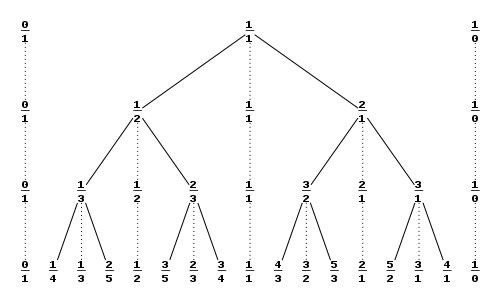
\includegraphics[scale=0.8]{images/sbtree.png}
	\label{fig:SBtree}
\end{figure}

$(\frac{b}{a},\frac{d}{c})$ 开区间
\begin{lstlisting}[language=C++]
void DFS(ll a,ll b,ll c,ll d,ll la,ll lb,ll ra,ll rb,ll x,ll y){
	if(b*x<a*y&&d*x>c*y){
		ans=mp(x,y);
		return ;
	}
	if(x>(int)1e9){
		ans=mp(-1ll,-1ll);
		return;
	}
	ll k;
	if(b*x>=a*y){
		k=(b*x-a*y)/(a*rb-b*ra)+1;
		DFS(a,b,c,d,x+(k-1)*ra,y+(k-1)*rb,ra,rb,x+k*ra,y+k*rb);
	}
	else {
        k=-(d*x-c*y)/-(c*lb-d*la)+1;
		DFS(a,b,c,d,la,lb,x+(k-1)*la,y+(k-1)*lb,x+k*la,y+k*lb);
	}
}
DFS(a,b,c,d,1,0,0,1,1,1);
\end{lstlisting}
$[\frac{b}{a},\frac{d}{c})$ 左闭右开
\begin{lstlisting}[language=Java]
public static void dfs(BigInteger a,BigInteger b,BigInteger c,BigInteger d,
    		BigInteger la,BigInteger lb,BigInteger ra,BigInteger rb,
    		BigInteger x,BigInteger y)
    {
        BigInteger le=b.multiply(x).subtract(a.multiply(y));
        BigInteger ri=d.multiply(x).subtract(c.multiply(y));
        if(le.compareTo(zero)<=0 && ri.compareTo(zero)>0)
        {
            ans=x;
            return ;
        }
        BigInteger k,tem;
        if(le.compareTo(zero)>0)
        {
            tem=a.multiply(rb).subtract(b.multiply(ra));
            k=le.add(tem.subtract(one)).divide(tem);
            dfs(a,b,c,d,
            x.add(k.subtract(one).multiply(ra)),y.add(k.subtract(one).multiply(rb)),
            ra,rb,
            x.add(k.multiply(ra)),y.add(k.multiply(rb)));
        }
        else
        {
            ri=ri.negate();
            tem=d.multiply(la).subtract(c.multiply(lb));
            k=ri.divide(tem).add(one);
            dfs(a,b,c,d,
            la,lb,
            x.add(k.subtract(one).multiply(la)),y.add(k.subtract(one).multiply(lb)),
            x.add(k.multiply(la)),y.add(k.multiply(lb)));
        }
    }
\end{lstlisting}
\subsection{类欧几里得算法}
\begin{eqnarray*}
	f&=&\sum_{i=0}^n\lfloor\frac{ai+b}{c}\rfloor\\
	g&=&\sum_{i=0}^ni\lfloor\frac{ai+b}{c}\rfloor\\
	h&=&\sum_{i=0}^n{\lfloor\frac{ai+b}{c}\rfloor}^2
\end{eqnarray*}

1e9不取模
\begin{lstlisting}[language=C++]
ll f(ll a,ll b,ll c,ll n)
{
    if (!c)return 0;
    if (a>=c||b>=c) return (a/c)*n*(n+1)/2+(b/c)*(n+1)+f(a%c,b%c,c,n);
    else return (a*n+b)/c*n-f(c,c-b-1,a,(a*n+b)/c-1);
}
\end{lstlisting}

1e18带取模
\begin{lstlisting}[language=C++]
typedef long long ll;
typedef __int128 lll;
const ll mod=998244353;
const ll inv2=(mod+1)/2;
ll sum(lll n)
{
    n%=mod;
    return 1LL*n*(n+1)%mod*inv2%mod;
}
ll f(ll a,ll b,ll c,lll n)
{
    if(!a) return (b/c)%mod*((n+1)%mod)%mod;
    if(a>=c||b>=c) return
        ((lll)(a/c)*sum(n)%mod+((b/c)%mod)*((n+1)%mod)%mod+f(a%c,b%c,c,n))%mod;
    lll m=((lll)a*n+b)/c;
    return ((m%mod)*(n%mod)%mod-f(c,c-b-1,a,m-1)+mod)%mod;
}
\end{lstlisting}

全部版本
\begin{lstlisting}[language=C]
ll inv2,inv6,a,b,c,l,r;
struct E
{
    ll f,g,h;
    E() {}
    E(ll _f,ll _g,ll _h)
    {
        f=_f,g=_g,h=_h;
    }
};
ll pow(ll a,ll b)
{
    ll t=1;
    for(; b; b>>=1,a=1LL*a*a%P)
        if(b&1)
            t=1LL*t*a%P;
    return t;
}
E cal(ll a,ll b,ll c,ll n)
{
    if (!a)return E(0,0,0);
    E x,y;
    if(a>=c||b>=c)
    {
        x=cal(a%c,b%c,c,n);
        y.f=(a/c*n%P*(n+1)%P*inv2+b/c*(n+1)+x.f)%P;
        y.g=(a/c*n%P*(n+1)%P*(n*2+1)%P*inv6+
             b/c*(n+1)%P*n%P*inv2+x.g)%P;
        y.h=a/c*(a/c)%P*n%P*(n+1)%P*(n*2+1)%P*inv6%P;
        (y.h+=b/c*(b/c)%P*(n+1))%=P;
        (y.h+=a/c*(b/c)%P*n%P*(n+1))%=P;
        (y.h+=2LL*(a/c)%P*x.g)%=P;
        (y.h+=2LL*(b/c)%P*x.f)%=P;
        (y.h+=x.h)%=P;
        y.f=(y.f+P)%P;
        y.g=(y.g+P)%P;
        y.h=(y.h+P)%P;
        return y;
    }
    ll m=(a*n+b)/c;
    x=cal(c,c-b-1,a,m-1);
    y.f=(n*m-x.f)%P;
    y.g=((n+1)*n%P*m-x.f-x.h)%P;
    y.g=y.g*inv2%P;
    y.h=(n*m%P*(m+1)-2LL*x.g-2LL*x.f-y.f)%P;
    y.f=(y.f+P)%P;
    y.g=(y.g+P)%P;
    y.h=(y.h+P)%P;
    return y;
}
int main()
{
    inv2=pow(2,P-2);
    inv6=pow(6,P-2);
    scanf("%lld%lld%lld%lld%lld",&a,&c,&b,&l,&r);
    printf("%lld",(cal(a,b,c,r).g-cal(a,b,c,l-1).g+P)%P);
}

\end{lstlisting}

\subsection{BM算法(orz dls)}
\begin{lstlisting}[language=C++]
#include <cstdio>
#include <cstring>
#include <cmath>
#include <algorithm>
#include <vector>
#include <string>
#include <map>
#include <set>
#include <cassert>
using namespace std;
#define rep(i,a,n) for (int i=a;i<n;i++)
#define per(i,a,n) for (int i=n-1;i>=a;i--)
#define pb push_back
#define mp make_pair
#define all(x) (x).begin(),(x).end()
#define fi first
#define se second
#define SZ(x) ((int)(x).size())
typedef vector<int> VI;
typedef long long ll;
typedef pair<int,int> PII;
const ll mod=1000000007;
ll powmod(ll a,ll b)
{ll res=1;a%=mod; assert(b>=0);for(;b;b>>=1){if(b&1)res=res*a%mod;a=a*a%mod;}return res;}
// head

int _;
namespace linear_seq {
    const int N=10010;
    ll res[N],base[N],_c[N],_md[N];

    vector<int> Md;
    void mul(ll *a,ll *b,int k) {
        rep(i,0,k+k) _c[i]=0;
        rep(i,0,k) if (a[i]) rep(j,0,k) _c[i+j]=(_c[i+j]+a[i]*b[j])%mod;
        for (int i=k+k-1;i>=k;i--) if (_c[i])
            rep(j,0,SZ(Md)) _c[i-k+Md[j]]=(_c[i-k+Md[j]]-_c[i]*_md[Md[j]])%mod;
        rep(i,0,k) a[i]=_c[i];
    }
    int solve(ll n,VI a,VI b) { // a 系数 b 初值 b[n+1]=a[0]*b[n]+...
//        printf("%d\n",SZ(b));
        ll ans=0,pnt=0;
        int k=SZ(a);
        assert(SZ(a)==SZ(b));
        rep(i,0,k) _md[k-1-i]=-a[i];_md[k]=1;
        Md.clear();
        rep(i,0,k) if (_md[i]!=0) Md.push_back(i);
        rep(i,0,k) res[i]=base[i]=0;
        res[0]=1;
        while ((1ll<<pnt)<=n) pnt++;
        for (int p=pnt;p>=0;p--) {
            mul(res,res,k);
            if ((n>>p)&1) {
                for (int i=k-1;i>=0;i--) res[i+1]=res[i];res[0]=0;
                rep(j,0,SZ(Md)) res[Md[j]]=(res[Md[j]]-res[k]*_md[Md[j]])%mod;
            }
        }
        rep(i,0,k) ans=(ans+res[i]*b[i])%mod;
        if (ans<0) ans+=mod;
        return ans;
    }
    VI BM(VI s) {
        VI C(1,1),B(1,1);
        int L=0,m=1,b=1;
        rep(n,0,SZ(s)) {
            ll d=0;
            rep(i,0,L+1) d=(d+(ll)C[i]*s[n-i])%mod;
            if (d==0) ++m;
            else if (2*L<=n) {
                VI T=C;
                ll c=mod-d*powmod(b,mod-2)%mod;
                while (SZ(C)<SZ(B)+m) C.pb(0);
                rep(i,0,SZ(B)) C[i+m]=(C[i+m]+c*B[i])%mod;
                L=n+1-L; B=T; b=d; m=1;
            } else {
                ll c=mod-d*powmod(b,mod-2)%mod;
                while (SZ(C)<SZ(B)+m) C.pb(0);
                rep(i,0,SZ(B)) C[i+m]=(C[i+m]+c*B[i])%mod;
                ++m;
            }
        }
        return C;
    }
    int gao(VI a,ll n) {
        VI c=BM(a);
        c.erase(c.begin());
        rep(i,0,SZ(c)) c[i]=(mod-c[i])%mod;
        return solve(n,c,VI(a.begin(),a.begin()+SZ(c)));
    }
};

int main() {
    ll n;
    while(scanf("%I64d",&n)!=EOF) {
        printf("%d\n",linear_seq::gao(VI{1,5,11,36,95,281},n-1));
    }
}

   	\end{lstlisting}
\subsection{自适应Simpson}

\begin{lstlisting}[language=C++]
double simpson(double a,double b) {
    double c = a + (b-a)/2;
    return (F(a) + 4*F(c) + F(b))*(b-a)/6;
}
double asr(double a,double b,double eps,double A) {
    double c = a + (b-a)/2;
    double L = simpson(a,c), R = simpson(c,b);
    if(fabs(L + R - A) <= 15*eps)return L + R + (L + R - A)/15.0;
    return asr(a,c,eps/2,L) + asr(c,b,eps/2,R);
}
double asr(double a,double b,double eps) {
    return asr(a,b,eps,simpson(a,b));
}
\end{lstlisting}
\subsection{单纯形算法}
\begin{itemize}
	\item n个(默认非负)实数变量,m个约束
	\item 第i个约束形如$ \sum_{j=1}^{n}a[i][j]\times x[j] \leq a[i][0] $
	\item 使目标函数$ \sum_{i=1}^{n}a[0][i] \times x[i]$最大
	\item 所有约束为大于等于,使目标函数最小,这时候需要对偶一下
	\item 目标$min{CX}$,约束$AX\geq B$,转化成目标$min{B^T Y}$,约束$A^T Y \leq C^T$,两个问题的最优解是相等的,且能保证目标函数取最优解时各个变量为整数
\end{itemize}
求$\max\{cx|Ax\leq b,x\geq0\}$的解。
\begin{lstlisting}[language=C++]
//from Claris,GP of Romania A.Balance
#include<cstdio>
#include<algorithm>
using namespace std;
typedef long long ll;
typedef vector<double>VD;
const int N=110;
const double eps=1e-9;
VD simplex(vector<VD>A, VD b, VD c){
    int n = A.size(), m = A[0].size() + 1, r = n, s = m - 1;
    vector<VD> D(n + 2, VD(m + 1, 0)); vector<int> ix(n + m);
    for(int i = 0; i < n + m; i ++) ix[i] = i;
    for(int i = 0; i < n; i ++){
        for(int j = 0; j < m - 1; j ++) D[i][j] = -A[i][j];
        D[i][m - 1] = 1; D[i][m] = b[i];
        if(D[r][m] > D[i][m]) r = i;
    }
    for(int j = 0; j < m - 1; j ++) D[n][j] = c[j];
    D[n + 1][m - 1] = -1;
    for(double d; ;){
        if(r < n){
            int t = ix[s]; ix[s] = ix[r + m]; ix[r + m] = t;
            D[r][s] = 1.0 / D[r][s]; vector<int> speedUp;
            for(int j = 0; j <= m; j ++) if(j != s){
                D[r][j] *= -D[r][s];
                if(D[r][j]) speedUp.push_back(j);
            }
            for(int i = 0; i <= n + 1; i ++) if(i != r){
                for(int j = 0; j < speedUp.size(); j ++)
                    D[i][speedUp[j]] += D[r][speedUp[j]] * D[i][s];
                D[i][s] *= D[r][s];
            }
        }
        r = -1; s = -1;
        for(int j = 0; j < m; j ++) if(s < 0 || ix[s] > ix[j])
            if(D[n + 1][j] > eps || (D[n + 1][j] > -eps && D[n][j] > eps)) s = j;
        if(s < 0) break;
        for(int i = 0; i < n; i ++) if(D[i][s] < -eps)
            if(r < 0 || (d = D[r][m] / D[r][s] - D[i][m] / D[i][s]) < -eps
                || (d < eps && ix[r + m] > ix[i + m])) r = i;
        if(r < 0) return VD();
    }//无边界
    if(D[n + 1][m] < -eps) return VD();//无解
    VD x(m - 1);
    for(int i = m; i < n + m; i ++) if(ix[i] < m - 1) x[ix[i]] = D[i - m][m];
    printf("%.0f\n",-D[n][m]);
    return x;
}//最优值在D[n][m]
int n,cnt,i,j,k;int a[N][N],f[N][N][N],s[N];double w[N];
int main(){
    scanf("%d",&n);
    for(i=1;i<=n;i++)for(j=1;j<=n;j++)scanf("%d",&a[i][j]);
    cnt=n*2-1;
    for(i=1;i<=n;i++){
        f[1][i][i]=1;
        if(i>1)f[i][1][i+n-1]=1;
    }
    for(i=2;i<=n;i++)for(j=2;j<=n;j++)for(k=1;k<=cnt;k++)f[i][j][k]=f[i-1][j][k]+f[i][j-1][k]-f[i-1][j-1][k];
    for(i=1;i<=n;i++)for(j=1;j<=n;j++)for(k=1;k<=cnt;k++)s[k]+=f[i][j][k];
    VD c;
    vector<VD>A;
    VD b;
    for(k=1;k<=cnt;k++)c.push_back(-s[k]);
    for(i=1;i<=n;i++)for(j=1;j<=n;j++){
        b.push_back(-a[i][j]);
        VD t;
        for(k=1;k<=cnt;k++)t.push_back(-f[i][j][k]);
        A.push_back(t);
    }
    VD ret=simplex(A,b,c);
    for(i=1;i<=cnt;i++)w[i]=ret[i-1];
    for(i=1;i<=n;puts(""),i++)for(j=1;j<=n;j++){
        double t=0;
        for(k=1;k<=cnt;k++)t+=w[k]*f[i][j][k];
        printf("%.0f ",t);
    }
}
\end{lstlisting}

下面的板可能有问题
\begin{lstlisting}[language=C++]
# define FOR(i, a, b) for (int i = a; i <= b; ++ i)
# define REP(i, n) FOR (i, 1, n)
# define REP_0N(i, n) FOR (i, 0, n)
# define N 110
# define M 110
typedef double ld;
const ld eps = 1e-8, inf = 1e9;
int n, m, id[N], tp[N];
ld a[M][N];
void pivot (int r, int c) {
    swap (id[r + n], id[c]);
    ld t = -a[r][c];
    a[r][c] = -1;
    REP_0N (i, n) a[r][i] /= t;
    REP_0N (i, m)
    if (a[i][c] && r != i) {
        t = a[i][c];
        a[i][c] = 0;
        REP_0N (j, n) a[i][j] += t * a[r][j];
    }
}
void solve () {
    ld t;
    REP (i, n) id[i] = i;
    while (true) {
        int i = 0, j = 0; ld w = -eps;
        REP (k, m) if (a[k][0] < w) w = a[i = k][0];
        if (!i) break;
        REP (k, n) if (a[i][k] > eps) {j = k;break;}
        if (!j) {printf ("Infeasible");return;}//不存在满足所有约束的解
        pivot (i, j);
    }
    while (true) {
        int i = 0, j = 0; ld w = eps;
        REP (k, n) if (a[0][k] > w) w = a[0][j = k];
        if (!j) break;
        w = inf;
        REP (k, m) if (a[k][j] < -eps && (t = -a[k][0] / a[k][j]) < w) w = t, i = k;
        if (!i) {printf ("Unbounded");return;}//目标函数无上界
        pivot (i, j);
    }
    printf ("%.9f\n", a[0][0]);
    FOR (i, n + 1, n + m) tp[id[i]] = i - n;
    REP (i, n) printf ("%.9f ", tp[i] ? a[tp[i]][0] : 0);
}
int main () {
    scanf ("%d%d", &n, &m);
    REP (i, n) scanf ("%lf", &a[0][i]);
    REP (i, m) {
        REP (j, n)
        scanf ("%lf", &a[i][j]), a[i][j] *= -1;
        scanf ("%lf", &a[i][0]);
    }
    solve ();
    return 0;
}

\end{lstlisting}

\section{数据结构}

\subsection{树上启发式}
\begin{lstlisting}[language=C++]
typedef vector<int> VI;
typedef long long LL;
typedef double db;
typedef pair<int,int> PII;

VI d[N],son[N];
PII maxl[N];

int id[N],ans[N],n,tot;

void add(int x){
    d[x].pb(1);
    maxl[x]=max(maxl[x],mp(1,(int)d[x].size()));
}
void merge(int y,int x){
    int n=d[y].size();
    int m=d[x].size();

    for(int i=0;i<n;i++){
        d[x][m-n+i]+=d[y][i];
        maxl[x]=max(maxl[x],mp(d[x][m-n+i],m-n+i+1));
    }
}
void DFS(int x,int fa){
    for(auto y:son[x])if(y!=fa)DFS(y,x);

    int hs=-1;
    for(auto y:son[x])if(y!=fa){
        if(hs==-1||d[id[hs]].size()<d[id[y]].size())hs=y;
    }
    if(hs!=-1)id[x]=id[hs];
    else id[x]=++tot;

    for(auto y:son[x])if(y!=fa&&y!=hs)merge(id[y],id[x]);
    add(id[x]);


    ans[x]=d[id[x]].size()-maxl[id[x]].se;
}
void __solve(){
	scanf("%d",&n);
    rep(i,1,n-1)
    {
        int u,v;
        scanf("%d%d",&u,&v);
        son[u].pb(v);
        son[v].pb(u);
    }
	DFS(1,0);
	rep(i,1,n)printf("%d\n",ans[i]);
}
int main()
{
	__solve();
	return 0;
}
\end{lstlisting}


\begin{lstlisting}[language=C++]
#define N 100010
#define INF
#define SZ(x) ((int)(x).size())

typedef vector<int> VI;
typedef long long LL;
typedef double db;
typedef pair<int,int> PII;

int sum[N],b[N],lev[N],siz[N];
int pos[N],maxl[4*N],ans[N];
int n,L;
VI son[N];

void DFS1(int x,int level){
	L=max(L,level);
	lev[x]=level;
	sum[level]+=b[x];
	siz[x]=1;
	for(auto y:son[x]){
		DFS1(y,level+1);
		siz[x]+=siz[y];
	}
}
inline void update(int x,int val){
	x=pos[x];
	maxl[x]=val;
	for(x>>=1;x;x>>=1)maxl[x]=max(maxl[x<<1],maxl[x<<1^1]);
}
void add(int x,int v,int ban){
	sum[lev[x]]+=v*b[x];
	update(lev[x],sum[lev[x]]);
	for(auto y:son[x])if(y!=ban)add(y,v,-1);
}
void DFS2(int x,int keep){
	int hs=-1;
	for(auto y:son[x])if(hs==-1||siz[y]>siz[hs])hs=y;
	for(auto y:son[x])if(y!=hs)DFS2(y,0);
	if(hs!=-1)DFS2(hs,1);
	add(x,-1,hs);
	ans[x]=maxl[1];
	if(!keep)add(x,1,-1);
}
void segment_tree (int l,int r,int k){
	if(l==r){maxl[k]=sum[l],pos[l]=k;return ;}
	int mid=l+r>>1;
	segment_tree(l,mid,k<<1);
	segment_tree(mid+1,r,k<<1^1);
	maxl[k]=max(maxl[k<<1],maxl[k<<1^1]);
}
void __solve(){
	int fa;
	scanf("%d",&n);
	rep(i,1,n)son[i].clear();
	memset(sum,0,4*n+40);
	rep(i,1,n)scanf("%d",&b[i]);
	rep(i,2,n)scanf("%d",&fa),son[fa].pb(i);
	DFS1(1,1);
	segment_tree(1,L,1);
	DFS2(1,0);
	rep(i,2,n)printf("%d\n",ans[i]);
}
int main()
{
	int T;
	scanf("%d",&T);
	while(T--)__solve();
	return 0;
}
\end{lstlisting}


\subsection{点分治}
\subsubsection{静态}
\begin{lstlisting}[language=C++]
/*
求树上距离小于D的点对数
*/
struct EDGE{
    int n,e;
}edge[N<<1];

int tot,fir[N],que[N],S,s[N],top,num[N],lev[N],vis[N],TT;
int LEV,f[N],siz[N],sz[N],n,l,r;

ll ans;
void add(int u,int v){
    edge[++tot].n=fir[u];
    fir[u]=tot;
    edge[tot].e=v;

    edge[++tot].n=fir[v];
    fir[v]=tot;
    edge[tot].e=u;
}
int getroot(int u){
    int Min=N,root=0;
    int hd,tl;
    hd=tl=0;
    que[tl++]=u;
    f[u]=0;
    for(;hd^tl;hd++){
        int x=que[hd];
        for(int u=fir[x];u;u=edge[u].n){
            int y=edge[u].e;
            if(y==f[x]||vis[y]==TT)continue;
            que[tl++]=y;
            f[y]=x;
        }
    }
    dow(i,tl-1,0){
        int x=que[i],Max=0;
        siz[x]=1;
        for(int u=fir[x];u;u=edge[u].n){
            int y=edge[u].e;
            if(y==f[x]||vis[y]==TT)continue;
            Max=max(Max,siz[y]);
            siz[x]+=siz[y];
        }
        Max=max(Max,tl-siz[x]);
        if(Max<Min)Min=Max,root=x;
    }
    return root;

}
int DFS2(int x,int f,int dep){
    int ret=dep;
    num[dep]++;
    s[++top]=x;
    lev[x]=dep;
    for(int u=fir[x];u;u=edge[u].n)if(vis[edge[u].e]!=TT&&edge[u].e!=f){
        ret=max(ret,DFS2(edge[u].e,x,dep+1));
    }
    return ret;
}
void work(int x,int D,int v){
    top=0;
    int dep=DFS2(x,0,D);
    rep(i,1,dep)num[i]+=num[i-1];
    rep(i,1,top){
        if(lev[s[i]]<=LEV)ans+=v*num[min(dep,-lev[s[i]]+LEV)];
    }
    rep(i,0,dep)num[i]=0;
}
void DIV(int x,int f){
    vis[x]=TT;
    work(x,0,1);
    int pre_sum=S;
    for(int u=fir[x];u;u=edge[u].n)if(vis[edge[u].e]!=TT){
        if(sz[edge[u].e]>sz[x])S=pre_sum-sz[x];
        else S=sz[edge[u].e];
        int root=getroot(edge[u].e);
        work(edge[u].e,1,-1);
        DIV(root,x);
    }
}

ll calc(ll x){
    if(x==n)return n;
    ans=0;
    LEV=n-1-x;
    TT++;
    S=n;
    DIV(getroot(1),0);
    return ans;
}
void __solve(){
    scanf("%d%d%d",&n,&l,&r);
    rep(i,1,n)fir[i]=0;
    tot=0;
    rep(i,1,n-1){
        int u,v;
        scanf("%d%d",&u,&v);
        add(u,v);
    }
    printf("%lld\n",(calc(l)-calc(r+1))/2);
}
\end{lstlisting}
\subsubsection{动态}
\begin{lstlisting}[language=C++]
#define N 200010
#define LOGN 40
#define SZ(x) ((int)(x).size())
namespace fastIO {
    #define BUF_SIZE 100000
    //fread -> read
    bool IOerror = 0;
    inline char nc() {
        static char buf[BUF_SIZE], *p1 = buf + BUF_SIZE, *pend = buf + BUF_SIZE;
        if(p1 == pend) {
            p1 = buf;
            pend = buf + fread(buf, 1, BUF_SIZE, stdin);
            if(pend == p1) {
                IOerror = 1;
                return -1;
            }
        }
        return *p1++;
    }
    inline bool blank(char ch) {
        return ch == ' ' || ch == '\n' || ch == '\r' || ch == '\t';
    }
    inline void getint(int &x) {
        char ch;
        while(blank(ch = nc()));
        if(IOerror) return;
        for(x = ch - '0'; (ch = nc()) >= '0' && ch <= '9'; x = x * 10 + ch - '0');
    }
    #undef BUF_SIZE
};
using namespace fastIO;
typedef vector<int> VI;
typedef long long ll;
typedef double db;
typedef pair<int,int> PII;
struct Edge
{
    int e,n;
}edge[N*2];

int sum[2][N*LOGN];
int st[2][N],ed[2][N],tot,TT,n,lt[2];
int dfn[N],deep[N],fa[N],num[N],fir[N],son[N],rev[N];
int idx,top[N],que[N],f[N],par[N],siz[N],sz[N],vis[N];
int ans;
void add(int u,int v){
    edge[++tot].n=fir[u];
    fir[u]=tot;
    edge[tot].e=v;

    edge[++tot].n=fir[v];
    fir[v]=tot;
    edge[tot].e=u;
}
int calc_up(int x,int len){
    while(len){
        if(deep[x]-deep[top[x]]>=len)return rev[dfn[x]-len];
        len-=deep[x]-deep[top[x]]+1,x=fa[top[x]];
    }
    return x;
}
int calc_lca(int x,int y){
    int f1=top[x],f2=top[y];
    while(f1!=f2)
    {
        if(deep[f1]<deep[f2])
        {
            swap(x,y);
            swap(f1,f2);
        }
        x=fa[f1];
        f1=top[x];
    }
    if(deep[x]>deep[y]) swap(x,y);
    return x;
}
void dfs(int x,int pre,int d){
    deep[x]=d;
    fa[x]=pre;
    num[x]=1;
    for(int u=fir[x];u;u=edge[u].n)if(edge[u].e!=pre)
    {
        dfs(edge[u].e,x,d+1);
        num[x]+=num[edge[u].e];
        if(son[x]==-1 || num[edge[u].e]>num[son[x]])
            son[x]=edge[u].e;
    }
}
void dfs_son(int x,int root)
{
    dfn[x]=++idx;
    rev[idx]=x;
    top[x]=root;
    if(son[x]==-1) return;
    else dfs_son(son[x],root);
    for(int u=fir[x];u;u=edge[u].n)
        if(edge[u].e!=fa[x] && edge[u].e!=son[x])
            dfs_son(edge[u].e,edge[u].e);
}
int getroot(int u)
{
    int Min=N,root=0;
    int hd,tl;
    hd=tl=0;
    que[tl++]=u;
    f[u]=0;
    for(; hd^tl; hd++)
    {
        int x=que[hd];
        for(int u=fir[x]; u; u=edge[u].n)
        {
            int y=edge[u].e;
            if(y==f[x]||vis[y]==TT)
                continue;
            que[tl++]=y;
            f[y]=x;
        }
    }
    dow(i,tl-1,0)
    {
        int x=que[i],Max=0;
        siz[x]=1;
        for(int u=fir[x]; u; u=edge[u].n)
        {
            int y=edge[u].e;
            if(y==f[x]||vis[y]==TT)
                continue;
            Max=max(Max,siz[y]);
            siz[x]+=siz[y];
        }
        Max=max(Max,tl-siz[x]);
        if(Max<Min)
            Min=Max,root=x;
    }
    return root;
}
int solve(int *sum,int &lt,int x,int f,int dep){
    if(x<=n)sum[dep+lt]++;
    int ret=dep;
    for(int u=fir[x];u;u=edge[u].n)if(edge[u].e!=f&&vis[edge[u].e]!=TT){
        ret=max(ret,solve(sum,lt,edge[u].e,x,dep+1));
    }
    return ret;
}

void work(int *st,int *ed,int &lt,int *sum,int x,int s,int D){
    st[x]=++lt;
    int dep=solve(sum,lt,s,0,D);
    rep(i,1,dep){
        ++lt;
        sum[lt]+=sum[lt-1];
    }
    ed[x]=lt;
}
void MID(int u,int v,int &mid,int &len){
    int lca=calc_lca(u,v);
    len=deep[u]+deep[v]-2*deep[lca];
    if(len/2<=deep[u]-deep[lca])mid=calc_up(u,len/2);
    else mid=calc_up(v,len/2);
}
int S;
int dis(int u,int v){
    int lca=calc_lca(u,v);
    return deep[u]+deep[v]-2*deep[lca];
}
void DIV(int x,int f){
    par[x]=f,vis[x]=TT;
    work(st[0],ed[0],lt[0],sum[0],x,x,0);
    int pre_sum=S;
    for(int u=fir[x];u;u=edge[u].n)if(vis[edge[u].e]!=TT){
        if(sz[edge[u].e]>sz[x])S=pre_sum-sz[x];
        else S=sz[edge[u].e];
        int root=getroot(edge[u].e);
        par[root]=x;//静态点分治可以去掉,直接在当前重心操作
        work(st[1],ed[1],lt[1],sum[1],root,edge[u].e,1);
        DIV(root,x);
    }
}

inline int CNT(int *sum,int *st,int *ed,int x,int len,int ct){
    if(len<0)return 0;
    return sum[min(len,ed[x]-st[x])+st[x]]-sum[st[x]]+(ct<=n);
}

inline int query(int x,int len){
    int y=x;
    int ret=CNT(sum[0],st[0],ed[0],x,len,x);
    int d;
    while(par[x]){
        d=dis(y,par[x]);
        ret+=CNT(sum[0],st[0],ed[0],par[x],len-d,par[x]);
        ret-=CNT(sum[1],st[1],ed[1],x,len-d,par[x]+n);
        x=par[x];
    }
    return ret;
}
void __solve(){
    int q;
    getint(n);
    getint(q);
    memset(sum[1],0,4*lt[1]+40);
    memset(sum[0],0,4*lt[0]+40);
    memset(fir,0,8*n+40);
    memset(son,-1,8*n+40);
    TT++;
    ans=tot=idx=0;
    lt[0]=lt[1]=0;

    rep(i,1,n-1){
        int u,v;
        getint(u);
        getint(v);
        add(u,i+n);
        add(v,i+n);
    }
    dfs(1,0,1);
    dfs_son(1,1);

    S=num[1];
    TT++;
    DIV(getroot(1),0);

    while(q--){
        int u,v,w;
        getint(u),getint(v),getint(w);
        u=(u+ans)%n+1,v=(v+ans)%n+1,w=(w+ans)%n;
        if(w==0)ans=(u==v?1:2);
        else {
            int mid,len;
            MID(u,v,mid,len);
            ans=query(u,2*w)+query(v,2*w)-query(mid,2*w-len/2);
        }
        printf("%d\n",ans);
    }
}
int main ()
{
    freopen("in.in","r",stdin);
    freopen("out.out","w",stdout);
    int T;
    getint(T);

    while(T--)__solve();
    return 0;
}
\end{lstlisting}

\subsection{并查集}
\subsubsection*{带权并查集/种类并查集}
\begin{lstlisting}[language=C++]
int fa[N],dis[N];
void init()
{
    memset(dis,0,sizeof(dis));
    for(int i=1;i<=n;i++) fa[i]=i;
}
int getfa(int x)
{
    if(x==fa[x]) return x;
    int tem=getfa(fa[x]);
    dis[x]+=dis[fa[x]];
    dis[x]%=300;
    return fa[x]=tem;
}
bool Merge(int x,int y,int c)//x->y c
{
    int fx=getfa(x),fy=getfa(y);
    if(fx==fy && dis[x]!=(dis[y]+c)%300) return false;
    fa[fx]=fy;
    dis[fx]=(c+dis[y]-dis[x]+300)%300;
    return true;
}
        \end{lstlisting}
\subsubsection*{带撤销并查集}
\begin{lstlisting}[language=C++]
int Find(int x)
{
    while(x!=fa[x]) x=fa[x];
    return x;
}
void Union(int x,int y,bool flag)
{
    x=Find(x);y=Find(y);
    if(rk[x]<rk[y]) swap(x,y);
    if(flag) stk.push(y);
    fa[y]=x;
    if(rk[x]==rk[y])
        ++rk[x];
}
void undo()
{
    while(!stk.empty())
    {
        fa[stk.top()]=stk.top();
        stk.pop();
    }
}
    \end{lstlisting}
h   \subsubsection*{离线LCA 树上路径查询}
2017 西安网络赛A TREE

树上每个点有个01矩阵,询问树上两点从x到y的矩阵乘积,模2意义下
这种信息只能合并不能做减法,即不能乘逆矩阵。可以用bitset加速矩阵乘法,并查集求出路径上矩阵乘积,注意要开二维,乘法有方向。时间复杂度$O(64^{2}N+64^{2}Q)$
\begin{lstlisting}[language=C++]
#include<bits/stdc++.h>
using namespace std;
#define N 30010
typedef unsigned long long ull;
typedef long long ll;
const ll mod=19260817;
const ll mod2=mod*mod;
int p19[66],p26[66];
int _e,_p[N],_last[N<<1],_head[N<<1],_w[N<<1],_dir[N<<1];
vector<int> edge[N];
int fa[2][N],lca[N];
bool vis[N];
int n,m;
ull seed;

struct node
{
    int x,i,o;
};
vector<node> que[N];
struct matrix64
{
    bitset<64> mx[64],my[64];
    matrix64()
    {
        for(int i=0;i<64;++i)
            mx[i].reset(),my[i].reset();
    }
    void clear()
    {
        for(int i=0;i<64;++i)
            mx[i].reset(),my[i].reset();
    }
    void init()
    {
        for(int i=0;i<64;++i)
            mx[i].reset(),my[i].reset();
        for(int i=0;i<64;++i)
            mx[i][i]=my[i][i]=1;
    }
    void set(int x,int y)
    {
        mx[x][y]=1;
        my[y][x]=1;
    }
    friend matrix64 operator *(const matrix64 &a,const matrix64 &b)
    {
        matrix64 c;
        bitset<64> tmp;
        for(int i=0;i<64;++i)
            for(int j=0;j<64;++j)
            {
                tmp=a.mx[i]&b.my[j];
                if(tmp.count()&1)
                {
                    c.mx[i][j]=1;
                    c.my[j][i]=1;
                }
            }
        return c;
    }
} A[N],dis[2][N],ans[2][N];

void addquery(int x,int y,int c,int o)
{
    _head[++_e]=y;_w[_e]=c;_dir[_e]=o;
    _last[_e]=_p[x];
    _p[x]=_e;
}

int getfa(int x,int o)
{
    if(x==fa[o][x]) return x;
    int rt=getfa(fa[o][x],o);
    if(o==0) dis[o][x]=dis[o][x]*dis[o][fa[o][x]];
    else dis[o][x]=dis[o][fa[o][x]]*dis[o][x];
    return fa[o][x]=rt;
}
void dfs(int x,int pre)
{
    fa[0][x]=x;fa[1][x]=x;
    dis[0][x].init();dis[1][x].init();
    vis[x]=true;
    for(int i=0;i<edge[x].size();++i)
    {
        int y=edge[x][i];
        if(y!=pre)
        {
            dfs(y,x);
            fa[0][y]=x;fa[1][y]=x;
            dis[0][y]=A[y];dis[1][y]=A[y];
        }
    }
    for(int j=_p[x];j;j=_last[j])
    {
        int y=_head[j];
        int i=_w[j],o=_dir[j];
        if(vis[y])
        {
            lca[i]=getfa(y,o);
            ans[o][i]=dis[o][y];
            que[lca[i]].push_back(node{x,i,o^1});
        }
    }
    for(auto &pr:que[x])
    {
        getfa(pr.x,pr.o);
        ans[pr.o][pr.i]=dis[pr.o][pr.x];
    }
}
int calc(matrix64 &tmp)
{
    ll now=0;
    for(int j=0;j<64;++j)
        for(int k=0;k<64;++k)
        if(tmp.mx[j][k])
        {
            now=(now+1LL*p19[j+1]*p26[k+1]);
            if(now>=mod2) now-=mod2;
        }
    return now%mod;
}
int main()
{
    p19[0]=p26[0]=1;
    for(int i=1;i<=64;++i)
    {
        p19[i]=19LL*p19[i-1]%mod;
        p26[i]=26LL*p26[i-1]%mod;
    }
    while(scanf("%d%d",&n,&m)!=EOF)
    {
        _e=0;
        for(int i=1;i<=n;++i)
        {
            _p[i]=0;
            edge[i].clear();
            que[i].clear();
        }
        for(int i=1;i<n;++i)
        {
            int x,y;
            scanf("%d%d",&x,&y);
            edge[x].push_back(y);
            edge[y].push_back(x);
        }
        scanf("%llu",&seed);
        for(int i=1;i<=n;++i)
        {
            A[i].clear();
            for(int j=0;j<64;++j)
            {
                seed^=seed*seed+15;
                for(int k=0;k<64;++k)
                if((seed>>k)&1)
                    A[i].set(j,k);
            }
        }
        for(int i=1;i<=m;++i)
        {
            int x,y;
            scanf("%d%d",&x,&y);
            addquery(x,y,i,1);
            addquery(y,x,i,0);
            ans[0][i].init();
            ans[1][i].init();
        }
        for(int i=1;i<=n;++i) vis[i]=false;
        dfs(1,0);
        for(int i=1;i<=m;++i)
        {
            matrix64 tmp=ans[0][i]*A[lca[i]];
            tmp=tmp*ans[1][i];
            printf("%d\n",calc(tmp));
        }
    }
}
\end{lstlisting}
\subsection{Trie树}
\begin{lstlisting}[language=C++]
/*
poj 3630
*/
#include<cstdio>
#include<cstring>
#include<iostream>
using namespace std;
struct trie
{
    int next[10];
    bool got;
    void init()
    {
        memset(next,0,sizeof(next));
        got=false;
    }
} t[200010];
int sk,n,len,now,tot;
bool ans;
char s[20];
void insert(char *s)
{
    int now=0;
    int len=strlen(s);
    bool flag=true;
    for(int i=0; i<len; i++)
    {
        if(t[now].next[s[i]-'0']) now=t[now].next[s[i]-'0'];
        else
        {
            flag=false;
            t[now].next[s[i]-'0']=++tot;
            t[now=tot].init();
        }
        if(t[now].got) ans=false;
    }
    if(flag) ans=false;
    t[now].got=true;
}
int main()
{
    scanf("%d",&sk);
    while(sk--)
    {
        tot=0;
        t[0].init();
        scanf("%d",&n);
        ans=true;
        for(int i=1; i<=n; ++i)
        {
            scanf("%s",s);
            if(ans) insert(s);
        }
        if(ans) puts("YES");
        else puts("NO");
    }
}
        \end{lstlisting}
\subsection{可持久化trie}
bzoj 3261 最大异或和
\begin{lstlisting}[language=C++]
#include<bits/stdc++.h>
using namespace std;
#define N 600010
int n,m;
int a[N],sum[N];
struct TRIE
{
    int tot;
    int root[N],rpos[N*32];
    int son[N*32][2];
    int newnode(int k)
    {
        rpos[++tot]=k;
        son[tot][0]=son[tot][1]=0;
        return tot;
    }
    void insert(int last,int y,int k)
    {
        int now=newnode(k);
        root[k]=now;
        for(int i=30; i>=0; --i)
        {
            int j=(y>>i)&1;
            son[now][j^1]=son[last][j^1];
            now=son[now][j]=newnode(k);
            last=son[last][j];
        }
    }
    int ask(int l,int r,int x)
    {
        int now=root[r],ans=0;
        for(int i=30; i>=0; --i)
        {
            int j=((x>>i)&1)^1;
            if(rpos[son[now][j]]>=l) ans|=1<<i;
            else j=j^1;
            now=son[now][j];
        }
        return ans;
    }
} trie;

int main()
{
    scanf("%d%d",&n,&m);
    trie.insert(trie.root[0],0,1);
    for(int i=1; i<=n; ++i)
    {
        scanf("%d",a+i);
        sum[i]=sum[i-1]^a[i];
        trie.insert(trie.root[i],sum[i],i+1);
    }
    while(m--)
    {
        char opt[4];
        scanf("%s",opt);
        if(opt[0]=='A')
        {
            scanf("%d",&a[++n]);
            sum[n]=sum[n-1]^a[n];
            trie.insert(trie.root[n],sum[n],n+1);
        }
        else
        {
            int l,r,x;
            scanf("%d%d%d",&l,&r,&x);
            printf("%d\n",trie.ask(l,r,x^sum[n]));
        }
    }
    return 0;
}

\end{lstlisting}

\begin{lstlisting}[language=C++]
#include<cstdio>
#include<cstring>
#include<iostream>
using namespace std;
#define N 100010
struct trie
{
    int son[2];
} t[N*32];
int e,head[N*2],last[N*2],p[N];
int d[N],root[N],pos[N],rpos[N*32];
int a[N];
int top[N],num[N],son[N],fa[N];
int n,m,tot,dfstime;
void add(int x,int y)
{
    head[++e]=y;
    last[e]=p[x];
    p[x]=e;
}
void insert(int last,int y,int k)
{
    int now;
    root[k]=now=++tot;
    rpos[now]=k;
    for(int i=30; i>=0; --i)
    {
        int j=(y>>i)&1;
        t[now].son[j^1]=t[last].son[j^1];
        t[now].son[j]=++tot;
        rpos[now=tot]=k;
        last=t[last].son[j];
    }
}
int ask(int l,int r,int x)
{
    int now=root[r],ans=0;
    for(int i=30; i>=0; --i)
    {
        int j=((x>>i)&1)^1;
        if(rpos[t[now].son[j]]>=l) ans|=1<<i;
        else j=j^1;
        now=t[now].son[j];
    }
    return ans;
}
void dfs(int pre,int x)
{
    pos[x]=++dfstime;
    d[x]=d[pre]+1;
    num[x]=1;
    fa[x]=pre;
    insert(root[pos[pre]],a[x],pos[x]);
    for(int j=p[x]; j; j=last[j])
        if(head[j]!=pre)
        {
            dfs(x,head[j]);
            num[x]+=num[head[j]];
            if(son[x]==-1 || num[head[j]]>num[son[x]])
                son[x]=head[j];
        }
}
void dfs_son(int x,int root)
{
    top[x]=root;
    if(son[x]==-1) return ;
    else dfs_son(son[x],root);
    for(int j=p[x];j;j=last[j])
        if(head[j]!=fa[x] && head[j]!=son[x])
            dfs_son(head[j],head[j]);
}
int LCA(int x,int y)
{
    int f1=top[x],f2=top[y];
    while(f1!=f2)
    {
        if(d[f1]<d[f2])
        {
            swap(x,y);
            swap(f1,f2);
        }
        x=fa[f1];
        f1=top[x];
    }
    if(d[x]>d[y]) swap(x,y);
    return x;
}
void init()
{
    e=0;
    memset(p,0,sizeof(p));
    dfstime=0;
    memset(root,0,sizeof(root));
    tot=0;
    memset(son,-1,sizeof(son));
}
int main()
{
    while(scanf("%d%d",&n,&m)!=EOF)
    {
        init();
        for(int i=1; i<=n; ++i) scanf("%d",a+i);
        for(int i=1; i<n; ++i)
        {
            int x,y;
            scanf("%d%d",&x,&y);
            add(x,y);
            add(y,x);
        }
        dfs(0,1);
        dfs_son(1,1);
        for(int i=1; i<=m; ++i)
        {
            int x,y,data;
            scanf("%d%d%d",&x,&y,&data);
            int lca=LCA(x,y);
            int ans=max(ask(pos[lca],pos[x],data),ask(pos[lca],pos[y],data));
            printf("%d\n",ans);
        }
    }
}
        \end{lstlisting}
\subsection{二进制分组+AC自动机}
\begin{lstlisting}[language=C++]
/*
http://codeforces.com/contest/710/problem/F String Set Queries
三个操作,往集合里插入、删除字符串,统计集合里的字符串在给定的字符串中出现多少次
保证不会加同样的串两次
插入和删除维护两个AC自动机,然后查询就是相减
但AC自动机不能动态的插入、查询,所以需要二进制分组
n个字符串的话,分成logn个组,每组大小是2的幂,每个串会被重建logn次
1:1
2:2
3:2 1
4:4
5:4 1
6:4 2
7:4 2 1
*/
#include<bits/stdc++.h>
using namespace std;
#define N 300010
#define MX 300010
typedef long long ll;
const int MBIT = 30;
struct lowbit_AC
{
    int son[MX][26], end[MX], fail[MX];
    int root[MBIT], size[MBIT], bitcnt, alloc;
    string str[N];
    int strcnt;
    void init()
    {
        alloc = strcnt = bitcnt = 0;
        memset(root, 0, sizeof(root));
        memset(size, 0, sizeof(size));
    }
    int newnode()
    {
        ++alloc;
        memset(son[alloc],0,sizeof(son[alloc]));
        end[alloc]=fail[alloc]=0;
        return alloc;
    }
    void build(int rt)
    {
        queue<int>q;
        fail[rt] = rt;
        for(int i = 0; i < 26; ++i)
        {
            if(!son[rt][i]) son[rt][i] = rt;
            else fail[son[rt][i]] = rt, q.push(son[rt][i]);
        }
        while(!q.empty())
        {
            int x = q.front();
            q.pop();
            end[x] += end[fail[x]];
            for(int i = 0; i < 26; ++i)
            {
                if(!son[x][i]) son[x][i] = son[fail[x]][i];
                else fail[son[x][i]] = son[fail[x]][i], q.push(son[x][i]);
            }
        }
    }
    void rebuild(int l, int r, int &rt)
    {
        rt = newnode();
        for(int i = l; i <= r; ++i)
        {
            int now = rt;
            for(int j = 0,len=str[i].length(); j < len; ++j)
            {
                if(son[now][str[i][j]-'a'] == 0) son[now][str[i][j]-'a'] = newnode();
                now = son[now][str[i][j]-'a'];
            }
            end[now]++;
        }
        build(rt);
    }
    void insert(char *s)
    {
        str[++strcnt]=string(s);
        size[++bitcnt]=1;
        root[bitcnt]=newnode();
        while(bitcnt >= 2 && size[bitcnt] == size[bitcnt-1])
            size[--bitcnt] *= 2;
        alloc = root[bitcnt]-1;
        rebuild(strcnt-size[bitcnt]+1, strcnt, root[bitcnt]);
    }
    ll query(char *s, int rt)
    {
        int now = rt;
        ll res = 0;
        for(int i = 0; s[i]; ++i)
        {
            now = son[now][s[i]-'a'];
            res += end[now];
        }
        return res;
    }
    ll ask(char *s)
    {
        ll res = 0;
        for(int i = 1; i <= bitcnt; ++i)
        {
            res += query(s, root[i]);
        }
        return res;
    }
} ac,de;
char s[N];
int main()
{
    int n;
    scanf("%d", &n);
    ac.init();
    de.init();
    for(int i = 0; i < n; ++i)
    {
        int opt;
        scanf("%d",&opt);
        scanf("%s",s);
        if(opt==1) ac.insert(s);
        else if(opt==2) de.insert(s);
        else printf("%lld\n", ac.ask(s)-de.ask(s)),fflush(stdout);
    }
}

    \end{lstlisting}
\subsection{线段树}
\begin{itemize}
	\item 区间加,区间乘,区间覆盖,区间求和,区间最值
	\item 线段树上二分
	\item 小清新线段树,区间加,区间除大概是$O(nlognlogC)$
	\item 优化建图,点$i$向区间$[L_i,R_i]$所有点连边。
\end{itemize}
\subsubsection{小清新线段树}
区间除法,支持权值为负,下取整,需根据区间最大最小值进行剪枝
\begin{lstlisting}[language=C++]
void Div(int p,int l,int r,int x)
{
    if(t[p].r<l || r<t[p].l || (t[p].min>=-1 && t[p].max<=0)) return;
    if(l<=t[p].l && t[p].r<=r && 
    (int)floor((double)t[p].min/x)-t[p].min==(int)floor((double)t[p].max/x)-t[p].max)
    {
        update(p,(int)floor((double)t[p].min/x)-t[p].min);
        return;
    }
    push_down(p);
    Div(ls(p),l,r,x);
    Div(rs(p),l,r,x);
    push_up(p);
}
\end{lstlisting}
区间取模,单点修改,区间求和,复杂度正确的原因$x mod y<\frac{x}{2}$
\begin{lstlisting}[language=C++]
void change(int p,int l,int r,int y)
{
    if(t[p].r<l||r<t[p].l||t[p].mx<y) return;
    if(t[p].l==t[p].r)
    {
        t[p].sum=t[p].mx=t[p].mx%y;
        return;
    }
    change(ls(p),l,r,y);
    change(rs(p),l,r,y);
    push_up(p);
}
\end{lstlisting}
\subsubsection{线段树优化建图}
bzoj 5017
Petrozavodsk Winter-2018. Carnegie Mellon U Contest A Mines
结合tarjan,DAG上dp
\begin{lstlisting}[language=C++]
void build(int &x,int l,int r)
{
    x=(l==r)?l:(++tot);
    if(l==r) return;
    int mid=l+r>>1;
    build(ls[x],l,mid);
    build(rs[x],mid+1,r);
    add(x,ls[x]);
    add(x,rs[x]);
}
void ins(int x,int l,int r,int L,int R,int y)
{
    if(L<=l && r<=R)
    {
        add(y,x);
        return;
    }
    int mid=l+r>>1;
    if(L<=mid) ins(ls[x],l,mid,L,R,y);
    if(mid<R) ins(rs[x],mid+1,r,L,R,y);
}

int main()
{
    //...
    tot=n;
    build(rt,1,n);
    for(int i=1;i<=n;++i)
    {
        int l=lower_bound(pos+1,pos+n+1,a[i].x-a[i].r)-pos;
        int r=upper_bound(pos+1,pos+n+1,a[i].x+a[i].r)-pos-1;
        ins(rt,1,n,l,r,i);
    }
    //tarjan
}
\end{lstlisting}

\subsubsection{线段树合并}
$O(nlogn)$
\begin{lstlisting}[language=C++]
/*
bzoj 2733 永无乡 
支持合并两个集合,查询一个集合内第k小的元素
*/
#include<bits/stdc++.h>
using namespace std;
#define N 100010
int tot;
int sum[N*20],ls[N*20],rs[N*20];
int fa[N],siz[N],root[N],id[N],val[N];
int n,m,q;
void insert(int &x,int y,int l,int r)
{
    ++sum[x=++tot];
    if(l==r) return;
    int mid=l+r>>1;
    if(y<=mid) insert(ls[x],y,l,mid);
    else insert(rs[x],y,mid+1,r);
}
int merge(int x,int y)
{
    if(!x||!y) return x+y;
    sum[x]=sum[x]+sum[y];
    ls[x]=merge(ls[x],ls[y]);
    rs[x]=merge(rs[x],rs[y]);
    return x;
}
int ask(int x,int y,int l,int r)
{
    if(l==r) return l;
    int mid=l+r>>1;
    if(y<=sum[ls[x]]) return ask(ls[x],y,l,mid);
    else return ask(rs[x],y-sum[ls[x]],mid+1,r);
}
int getfa(int x)
{
    return x==fa[x]?x:fa[x]=getfa(fa[x]);
}
void Union(int x,int y)
{
    x=getfa(x);y=getfa(y);
    if(x==y) return;
    if(siz[x]>siz[y]) swap(x,y);
    fa[x]=y;
    siz[y]+=siz[x];
    root[y]=merge(root[x],root[y]);
}
int Ask(int x,int y)
{
    x=getfa(x);
    if(siz[x]<y) return -1;
    return id[ask(root[x],y,1,n)];
}

int main()
{
    scanf("%d%d",&n,&m);
    tot=0;
    for(int i=1;i<=n;++i)
    {
        scanf("%d",&val[i]);id[val[i]]=i;
        fa[i]=i;
        siz[i]=1;
        insert(root[i],val[i],1,n);
    }
    for(int i=1;i<=m;++i)
    {
        int x,y;
        scanf("%d%d",&x,&y);
        Union(x,y);
    }
    scanf("%d",&q);
    while(q--)
    {
        char opt[3];
        int x,y;
        scanf("%s%d%d",opt,&x,&y);
        if(opt[0]=='Q') printf("%d\n",Ask(x,y));
        else Union(x,y);
    }
    return 0;
}
\end{lstlisting}

\subsection{莫队算法}
\subsubsection*{普通莫队}
\begin{lstlisting}[language=C++]
const int SIZE=300;
struct Q{int l,r,order;} q[N];
bool cmp(const re &a,const re &b)
{
    if(pos[a.l]!=pos[b.l]) return pos[a.l]<pos[b.l];
    return a.r<b.r;
}
int main()
{
    for(int i=1;i<=n;++i) pos[i]=(i-1)/SIZE+1;
    for(int i=1;i<=m;++i) q[i].order=i;
    sort(q+1,q+m+1,cmp);
    for(int i=1,l=1,r=0; i<=m; ++i)
    {
        int L=q[i].l ,R=q[i].r;
        while(r<R) add(++r);
        while(r>R) del(r--);
        while(l<L) del(l++);
        while(l>L) add(--l)
        ans[q[i].order]=now;
    }
    //for(int i=1; i<=m; ++i) print ans[i]
}
    \end{lstlisting}
\subsubsection*{带修改莫队}
因为查询操作只有在查询操作之前的所有修改操作完成之后才能保证正确性,
也就是说我只要记录了之前有多少个修改操作,然后在执行到当前查询的时候我把多进行的修改操作还原,
少进行的再进行修改就可以保证正确性。同时为了保证复杂度,采取的策略是对于每个询问按(l/block,r/block,time)排序(分别表示l所在的块、
r所在的询问之前的修改次数),再顺序完成,根据复杂度证明可以保证复杂度上界为n的三分之五次方。
\begin{lstlisting}[language=C++]
/*
bzoj 2120 数颜色
每次查询区间里有多少种不同的数,带单点修改
*/
#include<cstdio>
#include<iostream>
#include<cstring>
#include<cmath>
#include<algorithm>
using namespace std;
#define N 10010
struct Change
{
    int pos,color,pre;
} w[N];
struct Ask
{
    int l,r,id,time;
} q[N];
int numc,numq;
int pos[N],last[N];
int cnt[1000010],color[N],ans[N];
int now,n,m;
int size;
bool cmp(const Ask&a,const Ask&b)
{
    if(pos[a.l]!=pos[b.l]) return pos[a.l]<pos[b.l];
    if(pos[a.r]!=pos[b.r]) return pos[a.r]<pos[b.r];
    return a.time<b.time;
}
void insert(int x)
{
    now+=!(cnt[color[x]]++);
}
void erase(int x)
{
    now-=!(--cnt[color[x]]);
}
void change(int x,int l,int r,bool flag)
{
    int y=w[x].pos;
    if(l<=y && y<=r) erase(y);
    color[y]=flag?w[x].color:w[x].pre;
    if(l<=y && y<=r) insert(y);
}
void Mo()
{
    now=0;
    int l=1,r=0,curt=0;
    for(int i=1;i<=numq;i++)
    {
        while(curt<q[i].time) change(++curt,l,r,1);
        while(q[i].time<curt) change(curt--,l,r,0);
        while(l<q[i].l) erase(l++);
        while(q[i].l<l) insert(--l);
        while(q[i].r<r) erase(r--);
        while(r<q[i].r) insert(++r);
        ans[q[i].id]=now;
    }
}
int main()
{
    scanf("%d%d",&n,&m);
    for(int i=1;i<=n;i++)
        scanf("%d",&color[i]),last[i]=color[i];
    for(int i=1;i<=m;i++)
    {
        char s[10]; int x,y;
        scanf("%s",s);
        scanf("%d%d",&x,&y);
        if(s[0]=='R')
        {
            ++numc;
            w[numc].pos=x;
            w[numc].color=y;
            w[numc].pre=last[x];
            last[x]=y;
        }
        else
        {
            ++numq;
            q[numq].l=x;
            q[numq].r=y;
            q[numq].id=numq;
            q[numq].time=numc;
        }
    }
    size=sqrt(n);
    for(int i=1;i<=n;i++) pos[i]=(i-1)/size+1;
    sort(q+1,q+numq+1,cmp);
    Mo();
    for(int i=1;i<=numq;i++) printf("%d\n",ans[i]);
}
    \end{lstlisting}
\subsubsection*{回滚莫队}
当删除操作十分困难时可以存档,回滚处理
\begin{lstlisting}[language=C++]
/*
bzoj 4241 历史研究
每次查询区间里Max(x*num[x]),x表示所有的值,num[x]表示区间里x出现的次数,求最值显然无法直接删除
*/
#include<bits/stdc++.h>
using namespace std;
typedef long long ll;
#define N 100010
struct ask
{
    int l,r,o;
} q[N];
int n,m;
int a[N],hs[N],pos[N],num[N];
ll now;
ll ans[N];
bool cmp(const ask &a,const ask &b)
{
    if(pos[a.l]!=pos[b.l]) return pos[a.l]<pos[b.l];
    return a.r<b.r;
}
void del(int x)
{
    --num[a[x]];
}
void add(int x)
{
    ++num[a[x]];
    now=max(now,1LL*hs[a[x]]*num[a[x]]);
}
int main()
{
    scanf("%d%d",&n,&m);
    int siz=sqrt(n);
    for(int i=1;i<=n;++i)
    {
        scanf("%d",a+i);
        hs[i]=a[i];
        pos[i]=(i-1)/siz+1;
    }
    sort(hs+1,hs+n+1);
    int cnt=unique(hs+1,hs+n+1)-hs-1;
    for(int i=1;i<=n;++i)
        a[i]=lower_bound(hs+1,hs+cnt+1,a[i])-hs;
    for(int i=1;i<=m;++i)
    {
        scanf("%d%d",&q[i].l,&q[i].r);
        q[i].o=i;
    }
    sort(q+1,q+m+1,cmp);
    int r=0;
    for(int i=1;i<=m;++i)
    {
        int L=q[i].l,R=q[i].r;
        if(pos[q[i].l]!=pos[q[i-1].l])
        {
            memset(num,0,sizeof(num));
            r=pos[q[i].l]*siz;
            now=0;
        }
        while(r<R) add(++r);
        ll last=now;
        for(int j=L;j<=pos[q[i].l]*siz && j<=R;++j)
            add(j);
        ans[q[i].o]=now;
        //rollback
        for(int j=L;j<=pos[q[i].l]*siz && j<=R;++j)
            del(j);
        now=last;
    }
    for(int i=1;i<=m;++i)
        printf("%lld\n",ans[i]);
    return 0;
}
\end{lstlisting}
\subsection{主席树}
\begin{itemize}
	\item 可用于求区间第k大,区间小于某个值的数的个数(或者和),区间不同的数的个数等
\end{itemize}

\begin{lstlisting}[language=C++]
/*
SPOJ DQUERY
询问[l,r]有多少个不同的数
*/
#include <cstdio>
#include <cstring>
#include <iostream>
using namespace std;
#define N 30010
int sum[N*30],ls[N*30],rs[N*30];
int a[N],root[N];
int pos[1000010];
int n,m,tot;
void insert(int last,int &x,int y,int l,int r)
{
    sum[x=++tot]=sum[last]+1;
    ls[x]=ls[last];
    rs[x]=rs[last];
    if(l==r) return;
    int mid=l+r>>1;
    if(y<=mid) insert(ls[last],ls[x],y,l,mid);
    else insert(rs[last],rs[x],y,mid+1,r);
}
int ask(int ss,int tt,int l,int r,int y)
{
    if(l==r) return sum[tt]-sum[ss];
    int mid=l+r>>1;
    if(y<=mid) return ask(ls[ss],ls[tt],l,mid,y);
    else return sum[ls[tt]]-sum[ls[ss]]+ask(rs[ss],rs[tt],mid+1,r,y);
}
int main()
{
    scanf("%d",&n);
    for(int i=1; i<=n; i++)
    {
        scanf("%d",a+i);
        int x=a[i];
        a[i]=pos[x];
        pos[x]=i;
    }
    for(int i=1; i<=n; i++)
    {
        insert(root[i-1],root[i],a[i],0,n);
    }
    scanf("%d",&m);
    while(m--)
    {
        int l,r;
        scanf("%d%d",&l,&r);
        printf("%d\n",ask(root[l-1],root[r],0,n,l-1));
    }
}
    \end{lstlisting}
\subsection{替罪羊树}
\begin{lstlisting}[language=C++]
/*
bzoj 3224 普通平衡树
*/
#include<vector>
#include<cstring>
#include<cstdio>
#include<iostream>
using namespace std;
namespace Scapegoat_Tree {
    const int MAXN=100010;
  const double alpha = 0.75;
  struct Node {
  Node * ch[2];
  int key, size, cover; // size为有效节点的数量,cover为节点总数量
  bool exist; // 是否存在(即是否被删除)
  void PushUp(void) {
    size = ch[0]->size + ch[1]->size + (int)exist;
    cover = ch[0]->cover + ch[1]->cover + 1;
  }
  bool isBad(void) { // 判断是否需要重构
    return ((ch[0]->cover > cover * alpha + 5) ||
        (ch[1]->cover > cover * alpha + 5));
    }
  };
  struct STree {
  protected:
    Node mem_poor[MAXN]; //内存池,直接分配好避免动态分配内存占用时间
    Node *tail, *root, *null; // 用null表示NULL的指针更方便,tail为内存分配指针,root为根
    Node *bc[MAXN]; int bc_top; // 储存被删除的节点的内存地址,分配时可以再利用这些地址

    Node * NewNode(int key) {
      Node * p = bc_top ? bc[--bc_top] : tail++;
      p->ch[0] = p->ch[1] = null;
      p->size = p->cover = 1; p->exist = true;
      p->key = key;
      return p;
    }
    void Travel(Node * p, vector<Node *>&v) {
      if (p == null) return;
      Travel(p->ch[0], v);
      if (p->exist) v.push_back(p); // 构建序列
      else bc[bc_top++] = p; // 回收
      Travel(p->ch[1], v);
    }
    Node * Divide(vector<Node *>&v, int l, int r) {
      if (l >= r) return null;
      int mid = (l + r) >> 1;
      Node * p = v[mid];
      p->ch[0] = Divide(v, l, mid);
      p->ch[1] = Divide(v, mid + 1, r);
      p->PushUp(); // 自底向上维护,先维护子树
      return p;
    }
    void Rebuild(Node * &p) {
      static vector<Node *>v; v.clear();
      Travel(p, v); p = Divide(v, 0, v.size());
    }
    Node ** Insert(Node *&p, int val) {
      if (p == null) {
        p = NewNode(val);
        return &null;
      }
      else {
        p->size++; p->cover++;
        // 返回值储存需要重构的位置,若子树也需要重构,本节点开始也需要重构,以本节点为根重构
        Node ** res = Insert(p->ch[val >= p->key], val);
        if (p->isBad()) res = &p;
        return res;
      }
    }
    void Erase(Node *p, int id) {
      p->size--;
      int offset = p->ch[0]->size + p->exist;
      if (p->exist && id == offset) {
        p->exist = false;
        return;
      }
      else {
        if (id <= offset) Erase(p->ch[0], id);
        else Erase(p->ch[1], id - offset);
      }
    }
  public:
    void Init(void) {
      tail = mem_poor;
      null = tail++;
      null->ch[0] = null->ch[1] = null;
      null->cover = null->size = null->key = 0;
      root = null; bc_top = 0;
    }
    STree(void) { Init(); }

    void Insert(int val) {
      Node ** p = Insert(root, val);
      if (*p != null) Rebuild(*p);
    }
    int Rank(int val) {
      Node * now = root;
      int ans = 1;
      while (now != null) { // 非递归求排名
        if (now->key >= val) now = now->ch[0];
        else {
          ans += now->ch[0]->size + now->exist;
          now = now->ch[1];
        }
      }
      return ans;
    }
    int Kth(int k) {
      Node * now = root;
      while (now != null) { // 非递归求第K大
        if (now->ch[0]->size + 1 == k && now->exist) return now->key;
        else if (now->ch[0]->size >= k) now = now->ch[0];
        else k -= now->ch[0]->size + now->exist, now = now->ch[1];
      }
    }
    void Erase(int k) {
      Erase(root, Rank(k));
      if (root->size < alpha * root->cover) Rebuild(root);
    }
    void Erase_kth(int k) {
      Erase(root, k);
      if (root->size < alpha * root->cover) Rebuild(root);
    }
  };
}
using namespace Scapegoat_Tree;
void read(int &x)
{
    static char ch;bool neg=false;
    while(!isdigit(ch=getchar())) if(ch=='-') neg=true;
    x=ch-'0';
    while(isdigit(ch=getchar())) x=x*10+ch-'0';
    if(neg) x=-x;
}
STree t;
int main()
{
    int n;
    read(n);
    while(n--)
    {
        int opt,m;
        read(opt);read(m);
        if(opt==1) t.Insert(m);
        else if(opt==2) t.Erase(m);
        else if(opt==3) printf("%d\n",t.Rank(m));
        else if(opt==4) printf("%d\n",t.Kth(m));
        else if(opt==5) printf("%d\n",t.Kth(t.Rank(m)-1));
        else printf("%d\n",t.Kth(t.Rank(m+1)));
    }
}
         \end{lstlisting}
\subsection{Treap}
\begin{lstlisting}[language=C++]
/*
bzoj 3224
普通平衡树模板题
*/
#include <cstdio>
#include <cstdlib>
using namespace std;

const int oo=~0u>>1;

struct Treap{
    struct node{
        node* ch[2];
        int v,s,r,c;
        node(int v,node *t):v(v){ ch[0]=ch[1]=t; r=rand(); s=c=1; }
        bool operator < (const node &rhs) const { return r<rhs.r; }
        void push_up(){ s=ch[0]->s+ch[1]->s+c; }
    }*root,*null;
    Treap(){
        null=new node(0,0);
        null->s=null->c=0;
        null->r=oo;
        root=null;
    }
    void rotate(node* &o,bool d){
        node* k=o->ch[!d]; o->ch[!d]=k->ch[d]; k->ch[d]=o;
        o->push_up(); k->push_up(); o=k;
    }
    void insert(node* &o,int x){
        if(o==null) o=new node(x,null);
        else{
            if(o->v==x){
                o->c++; o->s++;
            }
            else{
                bool d=x>o->v;
                insert(o->ch[d],x);
                if(o->ch[d]<o) rotate(o,!d);
                o->push_up();
            }
        }
    }
    void remove(node* &o,int x){
        if(o->v==x){
            if(o->c>1) o->c--;
            else{
                if(o->ch[0]!=null&&o->ch[1]!=null){
                    bool d=o->ch[0]<o->ch[1];
                    rotate(o,d); remove(o->ch[d],x);
                }
                else{
                    node* u=o;
                    if(o->ch[0]==null) o=o->ch[1];
                    else o=o->ch[0];
                    delete u;
                }
            }
        }
        else{
            bool d=x>o->v;
            remove(o->ch[d],x);
        }
        if(o!=null) o->push_up();
    }
    int kth(node* o,int k){
        int s=o->ch[0]->s+o->c;
        if(k>o->ch[0]->s&&k<=s) return o->v;
        if(k<=o->ch[0]->s) return kth(o->ch[0],k);
        else return kth(o->ch[1],k-s);
    }
    int rank(node *o,int x){
        int s=o->ch[0]->s+o->c;
        if(x==o->v) return o->ch[0]->s+1;
        if(x<o->v) return rank(o->ch[0],x);
        else return s+rank(o->ch[1],x);
    }
    int pre(int x){
        node* t=root;
        int ret=0;
        while(t!=null){
            if(t->v<x){
                ret=t->v;
                t=t->ch[1];
            }
            else t=t->ch[0];
        }
        return ret;
    }
    int suc(int x){
        node *t=root;
        int ret=0;
        while(t!=null){
            if(t->v>x){
                ret=t->v;
                t=t->ch[0];
            }
            else t=t->ch[1];
        }
        return ret;
    }
}tree;

int main()
{
    int n,a,b;
    scanf("%d",&n);
    while(n--){
        scanf("%d%d",&a,&b);
        switch(a){
            case(1):tree.insert(tree.root,b);break;
            case(2):tree.remove(tree.root,b);break;
            case(3):printf("%d\n",tree.rank(tree.root,b));break;
            case(4):printf("%d\n",tree.kth(tree.root,b));break;
            case(5):printf("%d\n",tree.pre(b));break;
            case(6):printf("%d\n",tree.suc(b));break;
        }
    }
    return 0;
}
	\end{lstlisting}
\begin{lstlisting}[language=C++]
/*
内存池优化
*/
#include<bits/stdc++.h>
using namespace std;
#define N 100010
typedef pair<int,int> pr;
int n,m;
namespace Treap
{
    const int oo=~0U>>1;
    struct node
    {
        node* ch[2];
        int s,r,c;
        pr v;
        node(const pr &v_,node *t)
        {
            v=v_;
            ch[0]=ch[1]=t;
            r=1LL*rand()*rand()%100000;
            s=c=1;
        }
        void init(const pr &v_,node *t)
        {
            v=v_;
            ch[0]=ch[1]=t;
            r=1LL*rand()*rand()%100000;
            s=c=1;
        }
        bool operator <(const node &rhs)const
        {
            return r<rhs.r;
        }
        void push_up()
        {
            s=ch[0]->s+ch[1]->s+c;
        }
    }*root,*null;
    node *del[N];
    int tot;

    node* new_node(const pr &v_,node *t)
    {
        if(tot>0)
        {
            del[tot]->init(v_,t);
            return del[tot--];
        }
        else return new node(v_,t);
    }
    void init()
    {
        null=new node(make_pair(0,0),null);
        null->s=null->c=0;
        null->r=oo;
        root=null;
    }
    void rotate(node* &o,bool d)
    {
        node* k=o->ch[!d];
        o->ch[!d]=k->ch[d];
        k->ch[d]=o;
        o->push_up();
        k->push_up();
        o=k;
    }
    void insert(node* &o,const pr &x)
    {
        if(o==null) o=new_node(x,null);
        else
        {
            if(o->v==x)
            {
                o->c++;
                o->s++;
            }
            else
            {
                bool d=x > o->v;
                insert(o->ch[d],x);
                if(o->ch[d] < o) rotate(o,!d);
                o->push_up();
            }
        }
    }
    void remove(node* &o,const pr &x)
    {
        if(o->v==x)
        {
            if(o->c > 1) o->c--;
            else
            {
                if(o->ch[0]!=null && o->ch[1]!=null)
                {
                    bool d=o->ch[0]<o->ch[1];
                    rotate(o,d);
                    remove(o->ch[d],x);
                }
                else
                {
                    node* u=o;
                    if(o->ch[0]==null) o=o->ch[1];
                    else o=o->ch[0];
                    del[++tot]=u;//?
                }
            }
        }
        else
        {
            bool d=x>o->v;
            remove(o->ch[d],x);
        }
        if(o!=null) o->push_up();
    }
    int rank(node *o,const pr &x)
    {
        int s=o->ch[0]->s+o->c;
        if(x==o->v) return o->ch[0]->s+1;
        if(x<o->v) return rank(o->ch[0],x);
        else return s+rank(o->ch[1],x);
    }
    void insert(const pr &x)
    {
        insert(root,x);
    }
    void remove(const pr &x)
    {
        remove(root,x);
    }
    int rank(const pr &x)
    {
        return rank(root,x);
    }
}
pair<int,int> score[N];
int main()
{
    srand(time(0));
    Treap::init();
    scanf("%d%d",&n,&m);
    for(int i=1;i<=n;++i)
        Treap::insert(score[i]=make_pair(0,0));
    for(int i=1;i<=m;++i)
    {
        int x,y;
        scanf("%d%d",&x,&y);
        Treap::remove(score[x]);
        score[x].first--;
        score[x].second+=y;
        Treap::insert(score[x]);
        printf("%d\n",Treap::rank(score[1]));
    }
}
    \end{lstlisting}
\subsection{Splay}
\begin{lstlisting}[language=C++] 
/*
bzoj 1500 维修数列
插入,删除,修改,翻转,求和,求和最大的子列
*/
#include<cstdio>
#include<cstring>
#include<iostream>
#include<queue>
using namespace std;
#define L(x) t[x].son[0]
#define R(x) t[x].son[1]
#define LR t[t[root].son[1]].son[0]
#define inf (~0U>>2)
#define N 500010
struct splaytree{
    int son[2],pre,s;
    int key,ans,sum,ls,rs;
    bool rev,cov;
} t[N];
int a[N];
int n,m,tot,root;
queue<int> q;
inline int which(int x){return R(t[x].pre)==x;}
inline void sets(int pre,int x,int d){
    if(t[pre].son[d]=x) t[x].pre=pre;
}
int apply_new(){
    if(q.empty()) return (++tot);
    else {
        int x=q.front();q.pop();
        t[x].son[0]=t[x].son[1]=t[x].pre=0;t[x].s=1;
        t[x].key=t[x].sum=0;
        t[x].ans=t[x].ls=t[x].rs=-inf;
        t[x].rev=t[x].cov=0;
        return x;
    }
}
void update(int x){
    t[x].s=t[L(x)].s+t[R(x)].s+1;
    t[x].sum=t[L(x)].sum+t[R(x)].sum+t[x].key;
    t[x].ls=max(t[L(x)].ls,t[L(x)].sum+t[x].key+max(0,t[R(x)].ls));
    t[x].rs=max(t[R(x)].rs,t[R(x)].sum+t[x].key+max(0,t[L(x)].rs));
    t[x].ans=max(0,t[L(x)].rs)+t[x].key+max(0,t[R(x)].ls);
    t[x].ans=max(t[x].ans,t[L(x)].ans);
    t[x].ans=max(t[x].ans,t[R(x)].ans);
}
void update_rev(int x){
    if(x==0)return;
    t[x].rev^=1;
    swap(L(x),R(x));
    swap(t[x].ls,t[x].rs);
}
void update_cov(int x,int y){
    if(x==0)return;
    t[x].cov=1;
    t[x].key=y;
    t[x].sum=y*t[x].s;
    t[x].ls=t[x].rs=t[x].ans=max(t[x].sum,y);
}
void spread(int x){
    if(x==0)return;
    if(t[x].rev){
        update_rev(L(x));
        update_rev(R(x));
        t[x].rev=0;
    }
    if(t[x].cov){
        update_cov(L(x),t[x].key);
        update_cov(R(x),t[x].key);
        t[x].cov=0;
    }
}
void build(int &x,int pre,int l,int r){
    if(l>r)return;
    int mid=l+r>>1;
    t[x=apply_new()].pre=pre;
    t[x].s=1;
    t[x].rev=t[x].cov=0;
    t[x].key=t[x].sum=t[x].ans=t[x].ls=t[x].rs=a[mid];
    if(n!=inf) if(mid==0 || mid==n+1)
        t[x].ans=t[x].ls=t[x].rs=-inf;
    build(L(x),x,l,mid-1);
    build(R(x),x,mid+1,r);
    update(x);
}
void rot(int x){
    int pre=t[x].pre,d=which(x);
    spread(pre);
    spread(x);
    sets(pre,t[x].son[d^1],d);
    if(t[pre].pre==0) t[x].pre=0;
    else sets(t[pre].pre,x,which(pre));
    sets(x,pre,d^1);
    update(pre);
}
void splay(int x,int goal){
    while(t[x].pre!=goal){
        if(t[t[x].pre].pre==goal)
            rot(x);
        else if(which(x)==which(t[x].pre))
            {rot(t[x].pre);rot(x);}
        else{rot(x);rot(x);}
    }
    update(x);
    if(goal==0) root=x;
}
int find(int root,int k){
    int now=root,lsize;
    while(1){
        spread(now);
        lsize=t[L(now)].s;
        if(lsize+1==k) return now;
        else if(k<=lsize) now=L(now);
        else now=R(now),k-=lsize+1;
    }
}
void insert(int pos,int cnt){
    splay(find(root,pos+1),0);
    splay(find(root,pos+2),root);
    for(int i=1;i<=cnt;++i)scanf("%d",a+i);
    int rt;
    build(rt,0,1,cnt);
    LR=rt;t[rt].pre=R(root);
    update(R(root));
    update(root);
}
void del_save(int x){
    if(x==0)return;
    del_save(L(x));
    q.push(x);
    del_save(R(x));
}
void delet(int pos,int cnt){
    splay(find(root,pos),0);
    splay(find(root,pos+cnt+1),root);
    del_save(LR);
    t[LR].pre=0;
    LR=0;
    update(R(root));
    update(root);
}
void make_same(int pos,int cnt,int x){
    splay(find(root,pos),0);
    splay(find(root,pos+cnt+1),root);
    update_cov(LR,x);
    update(R(root));
    update(root);
}
void revers(int pos,int cnt){
    splay(find(root,pos),0);
    splay(find(root,pos+cnt+1),root);
    update_rev(LR);
    update(R(root));
    update(root);
}
int getsum(int pos,int cnt){
    splay(find(root,pos),0);
    splay(find(root,pos+cnt+1),root);
    return t[LR].sum;
}
int getans(int pos,int cnt){
    splay(find(root,pos),0);
    splay(find(root,pos+cnt+1),root);
    return t[LR].ans;
}

int main(){
    scanf("%d%d",&n,&m);
    for(int i=1;i<=n;++i) scanf("%d",a+i);
    build(root,0,0,n+1);
    t[0].ans=t[0].ls=t[0].rs=-inf;
    n=inf;
    while(m--){
        int pos,cnt,x;
        char opt[15];
        scanf("%s",opt);
        if(opt[0]=='I'){//insert
            scanf("%d%d",&pos,&cnt);
            insert(pos,cnt);
        }
        else if(opt[0]=='D'){//delete
            scanf("%d%d",&pos,&cnt);
            delet(pos,cnt);
        }
        else if(opt[0]=='M' && opt[2]=='K'){//make_same
            scanf("%d%d%d",&pos,&cnt,&x);
            make_same(pos,cnt,x);
        }
        else if(opt[0]=='R'){//reverse
            scanf("%d%d",&pos,&cnt);
            revers(pos,cnt); 
        }
        else if(opt[0]=='G'){//get_sum
            scanf("%d%d",&pos,&cnt);
            printf("%d\n",getsum(pos,cnt));
        }
        else printf("%d\n",getans(1,t[root].s-2));
    }
    return 0;
}

        \end{lstlisting}

\subsection{KDtree}
\begin{lstlisting}[language=C++]
/*
hdu2966 
二维平面n个点,求其他点与每个点最近的距离的平方
*/
#include<iostream>
#include<cstdio>
#include<cstring>
#include<queue>
#include<vector>
#include<algorithm>
using namespace std;
#define N 100010
#define ls(p) (p<<1)
#define rs(p) (p<<1 | 1)
const long long INF=1e18;
const int k=2;
int n,idx;
long long sqr(long long x)
{
    return x*x;
}
struct point
{
    int x[2];
    bool operator <(const point &t)const
    {
        return x[idx]<t.x[idx];
    }
    void input()
    {
        for(int i=0;i<k;i++)
            scanf("%d",&x[i]);
    }
    long long friend dist(const point &a,const point &b)
    {
        long long ans=sqr(a.x[0]-b.x[0])+sqr(a.x[1]-b.x[1]);
        return ans?ans:INF;
    }
}p[N],pc[N];
struct kdtree
{
    point pt[N<<2];
    bool son[N<<2];
    void build(int x,int l,int r,int dep)
    {
        if(l>r) return;
        son[x]=true;
        son[ls(x)]=son[rs(x)]=false;
        idx=dep%k;
        int mid=l+r>>1;
        nth_element(p+l,p+mid,p+r+1);
        pt[x]=p[mid];
        build(ls(x),l,mid-1,dep+1);
        build(rs(x),mid+1,r,dep+1);
    }
    long long query(int x,const point &p,int dep)
    {
        if(!son[x]) return INF;
        int idx=dep%k,ls=ls(x),rs=rs(x);
        long long now=dist(p,pt[x]),tem;
        if(p.x[idx]>=pt[x].x[idx]) swap(ls,rs);
        tem=query(ls,p,dep+1);
        if(tem>sqr(p.x[idx]-pt[x].x[idx]))
            tem=min(tem,query(rs,p,dep+1));
        return min(now,tem);
    }
} kd;
int main()
{
    scanf("%*d");
    while(scanf("%d",&n)!=EOF)
    {
        for(int i=0;i<n;i++) p[i].input(),pc[i]=p[i];
        kd.build(1,0,n-1,0);
        for(int i=0;i<n;i++)
            printf("%I64d\n",kd.query(1,pc[i],0));
    }
}
        \end{lstlisting}

\begin{lstlisting}[language=C++]
/*
hdu 4347
k维空间多组询问求最近的M个点
*/
#include<iostream>
#include<cstdio>
#include<cstring>
#include<queue>
#include<vector>
#include<algorithm>
using namespace std;
#define N 50010
#define ls(p) (p<<1)
#define rs(p) (p<<1 | 1)
const int inf=~0U>>2;
int n,k,idx;
struct point
{
    int x[5];
    bool operator <(const point &t)const
    {
        return x[idx]<t.x[idx];
    }
    void input()
    {
        for(int i=0;i<k;i++)
            scanf("%d",&x[i]);
    }
    void output()
    {
        for(int i=0;i<k;i++)
        {
            if(i) printf(" ");
            printf("%d",x[i]);
        }
        puts("");
    }
}p[N];
ztypedef pair<double,point> tp;
priority_queue<tp> nq;
int sqr(int x)
{
    return x*x;
}
struct kdtree
{
    point pt[N<<2];
    bool son[N<<2];
    void build(int x,int l,int r,int dep)
    {
        if(l>r) return;
        son[x]=true;
        son[ls(x)]=son[rs(x)]=false;
        idx=dep%k;
        int mid=l+r>>1;
        nth_element(p+l,p+mid,p+r+1);
        pt[x]=p[mid];
        build(ls(x),l,mid-1,dep+1);
        build(rs(x),mid+1,r,dep+1);
    }
    void query(int x,const point &p,int m,int dep)
    {
        if(!son[x]) return;
        tp nd(0,pt[x]);
        for(int i=0;i<k;i++)
            nd.first+=sqr(nd.second.x[i]-p.x[i]);
        int dim=dep%k,fg=0,ls=ls(x),rs=rs(x);
        if(p.x[dim]>=pt[x].x[dim]) swap(ls,rs);
        if(son[ls]) query(ls,p,m,dep+1);
        if(nq.size()<m) nq.push(nd),fg=1;
        else
        {
            if(nd.first<nq.top().first) nq.pop(),nq.push(nd);
            if(sqr(p.x[dim]-pt[x].x[dim])<nq.top().first) fg=1;
        }
        if(son[rs]&&fg) query(rs,p,m,dep+1);

    }
} kd;
int main()
{
    while(scanf("%d%d",&n,&k)!=EOF)
    {
        for(int i=0;i<n;i++) p[i].input();
        kd.build(1,0,n-1,0);
        int sk;
        scanf("%d",&sk);
        while(sk--)
        {
            int m;
            point t;
            t.input();
            scanf("%d",&m);
            kd.query(1,t,m,0);
            printf("the closest %d points are:\n", m);
            point pt[20];
            for(int j=0;!nq.empty();j++) pt[j]=nq.top().second,nq.pop();
            for(int j=m-1;j>=0;j--) pt[j].output();
        }
    }
}

        \end{lstlisting}
\subsection{cdq分治}
四维偏序,需保证每一维是个排列,数有多少对偏序关系
cdq分治套cdq分治,时间复杂度$O(nlog^{3}n)$
\begin{lstlisting}[language=C++]
#include<bits/stdc++.h>
using namespace std;
typedef long long ll;
#define N 50010
struct node
{
    int x,y,z;
    bool t;
} a[N],b[N],c[N];
int n;
ll ans;
struct BIT
{
    int c[N];
    void add(int x,int y)
    {
        for(;x<=n;x+=x&(-x)) c[x]+=y;
    }
    int ask(int x)
    {
        int ans=0;
        for(;x;x-=x&(-x)) ans+=c[x];
        return ans;
    }
}bit;
void cdq2(int l,int r)
{
    if(l==r) return;
    int mid=(l+r)>>1;
    cdq2(l,mid);
    cdq2(mid+1,r);
    int i=l,j=mid+1,k=l;
    while(i<=mid && j<=r)
    {
        if(b[i].y<b[j].y)
        {
            if(!b[i].t) bit.add(b[i].z,1);
            c[k++]=b[i++];
        }
        else
        {
            if(b[j].t) ans+=bit.ask(b[j].z);
            c[k++]=b[j++];
        }
    }
    while(i<=mid)
    {
        if(!b[i].t) bit.add(b[i].z,1);
        c[k++]=b[i++];
    }
    while(j<=r)
    {
        if(b[j].t) ans+=bit.ask(b[j].z);
        c[k++]=b[j++];
    }
    for(int i=l;i<=mid;++i) if(!b[i].t) bit.add(b[i].z,-1);
    for(int i=l;i<=r;++i) b[i]=c[i];
}
void cdq1(int l,int r)
{
    if(l==r) return;
    int mid=(l+r)>>1;
    cdq1(l,mid);
    cdq1(mid+1,r);
    int i=l,j=mid+1,k=l;
    while(i<=mid && j<=r)
    {
        if(a[i].x<a[j].x) b[k]=a[i++],b[k++].t=false;
        else b[k]=a[j++],b[k++].t=true;
    }
    while(i<=mid) b[k]=a[i++],b[k++].t=false;
    while(j<=r) b[k]=a[j++],b[k++].t=true;
    for(int i=l;i<=r;++i) a[i]=b[i];
    cdq2(l,r);
}
int main()
{
    while(scanf("%d",&n)!=EOF)
    {
        for(int i=1;i<=n;i++)scanf("%d",&a[i].x);
        for(int i=1;i<=n;i++)scanf("%d",&a[i].y);
        for(int i=1;i<=n;i++)scanf("%d",&a[i].z);
        ans=0;
        cdq1(1,n);
        printf("%lld\n",ans);
    }
}

        \end{lstlisting}
\subsection{询问离线分治}
使用条件询问可离线并且可以快速合并区间信息
比一般的线段树少个log并且好写
hdu 6328 Rectangle Radar Scanner
\begin{lstlisting}[language=C++]
#include<bits/stdc++.h>
using namespace std;
typedef long long ll;
#define N 100010
#define M 1000010
#define ls(p) (p<<1)
#define rs(p) (p<<1|1)
const int INF=0x3f3f3f3f;
struct segment
{
    int l,r;
    int min,max,prod;
} t[N<<2];
struct REC
{
    int xl,xr,yl,yr,o;
} rec[M],tmp[M];
int n,m,K;
int mn[M],mx[M],prod[M];
pair<int,int> val[N];
bool cmpl(const REC &a,const REC &b)
{
    return a.xl>b.xl;
}
bool cmpr(const REC &a,const REC &b)
{
    return a.xr<b.xr;
}
void push_up(int p)
{
    t[p].min=min(t[ls(p)].min,t[rs(p)].min);
    t[p].max=max(t[ls(p)].max,t[rs(p)].max);
    t[p].prod=1LL*t[ls(p)].prod*t[rs(p)].prod%K;
}
void build(int p,int l,int r)
{
    t[p].l=l;t[p].r=r;
    t[p].min=INF;
    t[p].max=-INF;
    t[p].prod=1;
    if(l==r) return;
    int mid=l+r>>1;
    build(ls(p),l,mid);
    build(rs(p),mid+1,r);
}
void insert(int p,int x,int y)
{
    if(t[p].l==t[p].r)
    {
        t[p].min=min(t[p].min,y);
        t[p].max=max(t[p].max,y);
        t[p].prod=1LL*t[p].prod*y%K;
        return;
    }
    int mid=t[p].l+t[p].r>>1;
    if(x<=mid) insert(ls(p),x,y);
    else insert(rs(p),x,y);
    push_up(p);
}
void ask(int p,int x)
{
    if(rec[x].yl<=t[p].l && t[p].r<=rec[x].yr)
    {
        int o=rec[x].o;
        mn[o]=min(mn[o],t[p].min);
        mx[o]=max(mx[o],t[p].max);
        prod[o]=1LL*prod[o]*t[p].prod%K;
        return;
    }
    int mid=t[p].l+t[p].r>>1;
    if(rec[x].yl<=mid) ask(ls(p),x);
    if(rec[x].yr>mid) ask(rs(p),x);
}
void travel(int p)
{
    if(t[p].min==INF) return;
    t[p].min=INF;
    t[p].max=-INF;
    t[p].prod=1;
    if(t[p].l==t[p].r) return;
    travel(ls(p));
    travel(rs(p));
}
void solve(int l,int r,int L,int R)
{
    if(l>r||L>R) return;
    int mid=l+r>>1;
    int x=L-1,y=R+1,now=L,j;
    for(int i=L;i<=R;++i)
        if(rec[i].xr<mid) tmp[++x]=rec[i];
        else if(rec[i].xl>mid) tmp[--y]=rec[i];
        else rec[now++]=rec[i];
    sort(rec+L,rec+now,cmpl);
    j=mid+1;
    for(int i=L;i<now;++i)
    {
        while(j>rec[i].xl)
        {
            --j;
            insert(1,val[j].first,val[j].second);
        }
        ask(1,i);
    }
    travel(1);
    sort(rec+L,rec+now,cmpr);
    j=mid;
    for(int i=L;i<now;++i)
    {
        while(j<rec[i].xr)
        {
            ++j;
            insert(1,val[j].first,val[j].second);
        }
        ask(1,i);
    }
    travel(1);
    for(int i=L;i<=x;++i) rec[i]=tmp[i];
    for(int i=y;i<=R;++i) rec[i]=tmp[i];
    solve(l,mid-1,L,x);
    solve(mid+1,r,y,R);
}
void read()
{
    int a[2],b[2],c[2],d[2];
    int p,q,r,mod;
    scanf("%d%d%d%d%d%d%d%d%d%d",&m,a,b,c,d,&p,&q,&r,&mod,&K);
    for(int i=1;i<=m;++i)
    {
        a[i&1]=(1LL*p*a[(i&1)^1]+1LL*q*b[(i&1)^1]+r)%mod;
        b[i&1]=(1LL*p*b[(i&1)^1]+1LL*q*a[(i&1)^1]+r)%mod;
        c[i&1]=(1LL*p*c[(i&1)^1]+1LL*q*d[(i&1)^1]+r)%mod;
        d[i&1]=(1LL*p*d[(i&1)^1]+1LL*q*c[(i&1)^1]+r)%mod;
        rec[i].xl=min(a[i&1]%n,b[i&1]%n)+1;
        rec[i].xr=max(a[i&1]%n,b[i&1]%n)+1;
        rec[i].yl=min(c[i&1]%n,d[i&1]%n)+1;
        rec[i].yr=max(c[i&1]%n,d[i&1]%n)+1;
        rec[i].o=i;
        mn[i]=INF;
        mx[i]=-INF;
        prod[i]=1;
    }
}
int main()
{
    int T;
    scanf("%d",&T);
    while(T--)
    {
        scanf("%d",&n);
        for(int i=1;i<=n;++i)
        {
            int x,y;
            scanf("%d%d",&x,&y);
            val[i]=make_pair(x,y);
        }
        build(1,1,n);
        read();
        solve(1,n,1,m);
        long long ans=0;
        for(int i=1;i<=m;++i)
        if(mn[i]!=INF)
            ans+=prod[i]^mx[i]^mn[i];
        printf("%lld\n",ans);
    }
    return 0;
}
\end{lstlisting}
\subsection{树链剖分}
\begin{itemize}
	\item 可以利用重链dfs序连续,代替倍增求点x往上跳k步的点是谁。
\end{itemize}
\begin{lstlisting}[language=C++]
/*
bzoj 1036
树,点权,单点修改,路径求最值,求和
*/
#include<cstring>
#include<iostream>
#include<cstdio>
using namespace std;
const int inf=~0U>>2;
#define N 30010
#define ls(p) (p<<1)
#define rs(p) (p<<1 | 1)
int head[N*2],last[N*2],p[N],e;
int deep[N],fa[N],num[N],son[N],top[N],pos[N],val[N];
int cnt,n,m;
struct segment
{
    int l,r,sum,mx;
} t[N*4];
void add(int x,int y)
{
    head[++e]=y;
    last[e]=p[x];
    p[x]=e;
}
void dfs1(int x,int pre,int d)
{
    deep[x]=d;
    fa[x]=pre;
    num[x]=1;
    for(int j=p[x];j;j=last[j])
    if(head[j]!=pre)
    {
        dfs1(head[j],x,d+1);
        num[x]+=num[head[j]];
        if(son[x]==-1 || num[head[j]]>num[son[x]])
            son[x]=head[j];
    }
}
void dfs2(int x,int root)
{
    top[x]=root;
    pos[x]=++cnt;
    if(son[x]==-1) return;
    else dfs2(son[x],root);
    for(int j=p[x];j;j=last[j])
    if(head[j]!=fa[x] && head[j]!=son[x])
        dfs2(head[j],head[j]);
}
void push_up(int p)
{
    t[p].mx=max(t[ls(p)].mx,t[rs(p)].mx);
    t[p].sum=t[ls(p)].sum+t[rs(p)].sum;
}
void build(int p,int l,int r)
{
    t[p].l=l;t[p].r=r;
    t[p].mx=t[p].sum=0;
    if(l==r) return;
    int mid=l+r>>1;
    build(ls(p),l,mid);
    build(rs(p),mid+1,r);
}
void change(int p,int x,int y)
{
    if(t[p].l==t[p].r)
    {
        t[p].mx=t[p].sum=y;
        return;
    }
    int mid=t[p].l+t[p].r>>1;
    if(x<=mid) change(ls(p),x,y);
    else change(rs(p),x,y);
    push_up(p);
}
int ask_max(int p,int l,int r){
    if(l<=t[p].l && t[p].r<=r) return t[p].mx;
    int mid=t[p].l+t[p].r>>1;
    int ans=-inf;
    if(l<=mid) ans=max(ans,ask_max(ls(p),l,r));
    if(mid<r)  ans=max(ans,ask_max(rs(p),l,r));
    return ans;
}
int ask_sum(int p,int l,int r)
{
    if(l<=t[p].l && t[p].r<=r) return t[p].sum;
    int mid=t[p].l+t[p].r>>1;
    int ans=0;
    if(l<=mid) ans+=ask_sum(ls(p),l,r);
    if(mid<r) ans+=ask_sum(rs(p),l,r);
    return ans;
}
int getmax(int x,int y)
{
    int f1=top[x],f2=top[y];
    int ans=-inf;
    while(f1!=f2)
    {
        if(deep[f1]<deep[f2])
        {
            swap(x,y);
            swap(f1,f2);
        }
        ans=max(ans,ask_max(1,pos[f1],pos[x]));
        x=fa[f1];
        f1=top[x];
    }
    if(x==y) return max(ans,val[x]);
    if(deep[x]>deep[y]) swap(x,y);
    return max(ans,ask_max(1,pos[x],pos[y]));
}
int getsum(int x,int y)
{
    int f1=top[x],f2=top[y];
    int ans=0;
    while(f1!=f2)
    {
        if(deep[f1]<deep[f2])
        {
            swap(x,y);
            swap(f1,f2);
        }
        ans+=ask_sum(1,pos[f1],pos[x]);
        x=fa[f1];
        f1=top[x];
    }
    if(x==y) return ans+val[x];
    if(deep[x]>deep[y]) swap(x,y);
    return ans+ask_sum(1,pos[x],pos[y]);
}
int main()
{
    scanf("%d",&n);
    for(int i=1;i<n;i++)
    {
        int x,y;
        scanf("%d%d",&x,&y);
        add(x,y);
        add(y,x);
    }
    for(int i=1;i<=n;i++)
    {
        scanf("%d",&val[i]);
    }
    memset(son,-1,sizeof(son));
    dfs1(1,0,0);
    dfs2(1,1);
    build(1,1,cnt);
    for(int i=1;i<=n;i++)
    {
        change(1,pos[i],val[i]);
    }
    scanf("%d",&m);
    while(m--)
    {
        char opt[10];
        int x,y;
        scanf("%s",opt);
        scanf("%d%d",&x,&y);
        if(opt[0]=='Q')
        {
            if(opt[1]=='M') printf("%d\n",getmax(x,y));
            else printf("%d\n",getsum(x,y));
        }
        else change(1,pos[x],val[x]=y);
    }
}

    \end{lstlisting}
\begin{lstlisting}[language=C++]
/*
hdu 5893
一棵无根树,两种操作:改变路径上的颜色,和询问路径上有多少段颜色。
序列上问题可以用线段树维护区间两端的颜色以及颜色段数,搬到树上只要树链剖分后用线段树维护即可。
*/
#include<cstring>
#include<cstdio>
#include<iostream>
#include<algorithm>
using namespace std;
#define N 40020
#define L(p) (p<<1)
#define R(p) (p<<1 | 1)
const int INF=~0U>>1;
struct segment
{
    int l,r,ans,ls,rs,cov;
} t[N*5];
int e,p[N*2],head[N*2],last[N*2],w[N*2];
int son[N],deep[N],top[N],fa[N],num[N],val[N],pos[N],rpos[N];
int cnt,lca;
int n,m;
struct node
{
    int ls,rs,ans;
    node(){}
    node(int ls_,int rs_,int ans_)
    {
        ls=ls_;
        rs=rs_;
        ans=ans_;
    }
};
void init()
{
    cnt=0;
    e=0;
    memset(p,0,sizeof(p));
    memset(son,-1,sizeof(son));
}
void add(int x,int y,int c)
{
    head[++e]=y;w[e]=c;
    last[e]=p[x];
    p[x]=e;
}
void dfs1(int x,int pre,int d)
{
    deep[x]=d;
    fa[x]=pre;
    num[x]=1;
    for(int j=p[x];j;j=last[j])
    if(head[j]!=pre)
    {
        val[head[j]]=w[j];
        dfs1(head[j],x,d+1);
        num[x]+=num[head[j]];
        if(son[x]==-1 || num[head[j]]>num[son[x]])
            son[x]=head[j];
    }
}
void dfs2(int x,int root)
{
    top[x]=root;
    pos[x]=++cnt;
    rpos[cnt]=x;
    if(son[x]==-1) return ;
    else dfs2(son[x],root);
    for(int j=p[x];j;j=last[j])
    if(head[j]!=fa[x] && head[j]!=son[x])
        dfs2(head[j],head[j]);
}
void push_up(int p)
{
    t[p].ans=t[L(p)].ans+t[R(p)].ans;
    if(t[L(p)].rs==t[R(p)].ls) t[p].ans--;
    t[p].ls=t[L(p)].ls;
    t[p].rs=t[R(p)].rs;
}
void update_cov(int p,int c)
{
    t[p].ans=1;
    t[p].ls=t[p].rs=c;
    t[p].cov=c;
}
void push_down(int p)
{
    if(t[p].cov!=INF)
    {
        update_cov(L(p),t[p].cov);
        update_cov(R(p),t[p].cov);
        t[p].cov=INF;
    }
}
void build(int p,int l,int r)
{
    t[p].l=l;t[p].r=r;t[p].cov=INF;
    if(l==r)
    {
        t[p].ans=1;
        t[p].ls=val[rpos[l]];
        t[p].rs=val[rpos[l]];
        return;
    }
    int mid=l+r>>1;
    build(L(p),l,mid);
    build(R(p),mid+1,r);
    push_up(p);
}
void change(int p,int l,int r,int c)
{
    if(l<=t[p].l && t[p].r<=r)
    {
        update_cov(p,c);
        return;
    }
    push_down(p);
    int mid=t[p].l+t[p].r>>1;
    if(l<=mid) change(L(p),l,r,c);
    if(mid<r) change(R(p),l,r,c);
    push_up(p);
}

node ask(int p,int l,int r)
{
    if(l<=t[p].l && t[p].r<=r)
    {
        return node(t[p].ls,t[p].rs,t[p].ans);
    }
    push_down(p);
    int mid=t[p].l+t[p].r>>1;
    node ans;
    if(r<=mid) ans=ask(L(p),l,r);
    else if(mid<l) ans=ask(R(p),l,r);
    else
    {
        node pl=ask(L(p),l,r);
        node pr=ask(R(p),l,r);
        ans=node(pl.ls,pr.rs,pl.ans+pr.ans-(int)(pl.rs==pr.ls));
    }
    push_up(p);
    return ans;
}
int LCA(int x,int y)
{
    int f1=top[x],f2=top[y];
    while(f1!=f2)
    {
        if(deep[f1]<deep[f2])
        {
            swap(x,y);
            swap(f1,f2);
        }
        x=fa[f1];
        f1=top[x];
    }
    if(deep[x]>deep[y]) swap(x,y);
    return x;
}
void tree_change(int x,int y,int c)
{
    int f1=top[x],f2=top[y];
    while(f1!=f2)
    {
        if(deep[f1]<deep[f2])
        {
            swap(x,y);
            swap(f1,f2);
        }
        change(1,pos[f1],pos[x],c);
        x=fa[f1];
        f1=top[x];
    }
    if(x==y) return;
    if(deep[x]>deep[y]) swap(x,y);
    change(1,pos[x]+1,pos[y],c);
}
int tree_ask(int x,int y)
{
    if(x==y) return 0;
    int f1=top[x],f2=top[y];
    int ans=0;
    int xc=INF,yc=INF;
    while(f1!=f2)
    {
        if(deep[f1]<deep[f2])
        {
            swap(x,y);
            swap(f1,f2);
            swap(xc,yc);
        }
        node now=ask(1,pos[f1],pos[x]);
        ans+=now.ans;
        if(now.rs==xc) ans--;
        xc=now.ls;
        x=fa[f1];
        f1=top[x];
    }
    if(x==y)
    {
        if(xc==yc)ans--;
        return ans;
    }
    if(deep[x]>deep[y])
    {
        swap(x,y);
        swap(xc,yc);
    }
    node now=ask(1,pos[x]+1,pos[y]);
    ans+=now.ans;
    if(now.ls==xc) ans--;
    if(now.rs==yc) ans--;
    return ans;
}
int main()
{
    while(scanf("%d%d",&n,&m)!=EOF)
    {
        init();
        for(int i=1;i<n;i++)
        {
            int x,y,c;
            scanf("%d%d%d",&x,&y,&c);
            add(x,y,c);
            add(y,x,c);
        }
        dfs1(1,0,0);
        dfs2(1,1);
        build(1,1,cnt);
        while(m--)
        {
            char opt[10];int x,y;
            scanf("%s",opt);
            scanf("%d%d",&x,&y);
            lca=LCA(x,y);
            if(opt[0]=='C')
            {
                int c;
                scanf("%d",&c);
                tree_change(x,y,c);
            }
            else
            {
                printf("%d\n",tree_ask(x,y));
            }
        }
    }
}

    \end{lstlisting}

\begin{lstlisting}[language=C++]
typedef vector<int> VI;
typedef long long LL;
typedef double db;
typedef pair<int,int> PII;

int sum[N],b[N],lev[N],siz[N];
int pos[N],maxl[4*N],ans[N];
int n,L;
VI son[N];

void DFS1(int x,int level)
{
    L=max(L,level);
    lev[x]=level;
    sum[level]+=b[x];
    siz[x]=1;
    for(auto y:son[x])
    {
        DFS1(y,level+1);
        siz[x]+=siz[y];
    }
}
inline void update(int x,int val)
{
    x=pos[x];
    maxl[x]=val;
    for(x>>=1; x; x>>=1)maxl[x]=max(maxl[x<<1],maxl[x<<1^1]);
}
void add(int x,int v,int ban)
{
    sum[lev[x]]+=v*b[x];
    update(lev[x],sum[lev[x]]);
    for(auto y:son[x])if(y!=ban)add(y,v,-1);
}
void DFS2(int x,int keep)
{
    int hs=-1;
    for(auto y:son[x])if(hs==-1||siz[y]>siz[hs])hs=y;
    for(auto y:son[x])if(y!=hs)DFS2(y,0);
    if(hs!=-1)DFS2(hs,1);
    add(x,-1,hs);
    ans[x]=maxl[1];
    if(!keep)add(x,1,-1);
}
void segment_tree (int l,int r,int k)
{
    if(l==r)
    {
        maxl[k]=sum[l],pos[l]=k;
        return ;
    }
    int mid=l+r>>1;
    segment_tree(l,mid,k<<1);
    segment_tree(mid+1,r,k<<1^1);
    maxl[k]=max(maxl[k<<1],maxl[k<<1^1]);
}
void __solve()
{
    int fa;
    scanf("%d",&n);
    rep(i,1,n)son[i].clear();
    memset(sum,0,4*n+40);
    rep(i,1,n)scanf("%d",&b[i]);
    rep(i,2,n)scanf("%d",&fa),son[fa].pb(i);
    DFS1(1,1);
    segment_tree(1,L,1);
    DFS2(1,0);
    rep(i,2,n)printf("%d\n",ans[i]);
}
int main()
{
    int T;
    scanf("%d",&T);
    while(T--)__solve();
    return 0;
}

\end{lstlisting}
\subsection{Link-Cut tree}
\subsubsection*{维护路径}
\begin{itemize}
	\item Link,Cut操作均无向,需保证合法
	\item Cut操作为以x为根,断掉y与父亲的边
	\item Splay完如果要向下走,需要每次pushdown标记
	\item bzoj 2002 弹飞绵羊 记splay中的子树大小size,Access(x),Splay(x),然后x的左子树大小即为到当前根的距离
	\item The Kunming-Singapore Railway 动态加边的最小生成树,边拆点,维护最大权值的编号。
\end{itemize}
\begin{lstlisting}[language=C++]
/*
hdu 4010
*/
#include<bits/stdc++.h>
using namespace std;
typedef long long ll;
#define L(x) son[x][0]
#define R(x) son[x][1]
#define N 300010

int n,m;
vector<int> e[N];

struct LCT
{
    int son[N][2],pre[N];
    int val[N],cov[N],maxval[N];
    int sta[N],tp;
    bool rev[N];
    void init(int n)
    {
        for(int i=0;i<=n;++i)
        {
            L(i)=R(i)=0;
            pre[i]=0;
            rev[i]=false;
            val[i]=cov[i]=maxval[i]=0;
        }
    }
    int which(int x)
    {
        return R(pre[x])==x;
    }
    void sets(int fa,int x,int d)
    {
        if(son[fa][d]=x) pre[x]=fa;
    }
    bool root(int x)
    {
        return (L(pre[x])!=x && R(pre[x])!=x);
    }
    void push_up(int x)
    {
        maxval[x]=val[x];
        if(L(x)) maxval[x]=max(maxval[x],maxval[L(x)]);
        if(R(x)) maxval[x]=max(maxval[x],maxval[R(x)]);
    }
    void update_rev(int x)
    {
        if(x==0) return;
        swap(L(x),R(x));
        rev[x]^=1;
    }
    void update_add(int x,int y)
    {
        if(x==0) return;
        val[x]+=y;
        cov[x]+=y;
        maxval[x]+=y;
    }
    void push_down(int x)
    {
        if(x==0) return;
        if(rev[x])
        {
            update_rev(L(x));
            update_rev(R(x));
            rev[x]=0;
        }
        if(cov[x])
        {
            update_add(L(x),cov[x]);
            update_add(R(x),cov[x]);
            cov[x]=0;
        }
    }

    void rot(int x)
    {
        int fa=pre[x],d=which(x);
        sets(fa,son[x][d^1],d);
        if(root(fa)) pre[x]=pre[fa];
        else sets(pre[fa],x,which(fa));
        sets(x,fa,d^1);
        push_up(fa);
    }
    void Relax(int x)
    {
        for(;!root(x);x=pre[x]) sta[++tp]=x;
        sta[++tp]=x;
        for(;tp;--tp) push_down(sta[tp]);
    }
    void Splay(int x)
    {
        Relax(x);
        while(!root(x))
            if(root(pre[x]))
                rot(x);
            else if(which(x)==which(pre[x]))
            {
                rot(pre[x]);
                rot(x);
            }
            else
            {
                rot(x);
                rot(x);
            }
        push_up(x);
    }
    int Access(int x)
    {
        int y=0;
        for(; x; x=pre[y=x])
        {
            Splay(x);
            sets(x,y,1);
            push_up(x);
        }
        return y;
    }
    int Find(int x)
    {
        for(x=Access(x);L(x);x=L(x));
        return x;
    }
    void Makeroot(int x)
    {
        Access(x);
        Splay(x);
        update_rev(x);
    }
    void Link(int x,int y)
    {
        Makeroot(x);
        pre[x]=y;
    }
    void Cut(int x,int y)
    {
        Makeroot(x);
        Access(y);
        Splay(y);
        pre[L(y)]=0;
        L(y)=0;
        push_up(y);
    }
    void Add(int x,int y,int c)
    {
        Makeroot(x);
        Access(y);
        Splay(y);
        update_add(y,c);
    }
    int Ask_max(int x,int y)
    {
        Makeroot(x);
        Access(y);
        Splay(y);
        return maxval[y];
    }
    bool isConnect(int x,int y)
    {
        return Find(x)==Find(y);
    }
} lct;

void dfs(int x,int fa)
{
    for(auto &y:e[x])
    if(y!=fa)
    {
        lct.pre[y]=x;
        dfs(y,x);
    }
}
int main()
{
    while(scanf("%d",&n)!=EOF)
    {
        lct.init(n);
        for(int i=0;i<=n;++i) e[i].clear();
        for(int i=1; i<n; i++)
        {
            int x,y;
            scanf("%d%d",&x,&y);
            e[x].push_back(y);
            e[y].push_back(x);
        }
        dfs(1,0);
        for(int i=1; i<=n; i++)
        {
            scanf("%d",&lct.val[i]);
            lct.maxval[i]=lct.val[i];
        }
        scanf("%d",&m);
        while(m--)
        {
            int opt,c,x,y;
            scanf("%d",&opt);
            if(opt==1)
            {
                scanf("%d%d",&x,&y);
                if(lct.isConnect(x,y)) puts("-1");
                else lct.Link(x,y);
            }
            else if(opt==2)
            {
                scanf("%d%d",&x,&y);
                if(x==y || !lct.isConnect(x,y)) puts("-1");
                else lct.Cut(x,y);
            }
            else if(opt==3)
            {
                scanf("%d%d%d",&c,&x,&y);
                if(!lct.isConnect(x,y)) puts("-1");
                else lct.Add(x,y,c);
            }
            else
            {
                scanf("%d%d",&x,&y);
                if(!lct.isConnect(x,y)) puts("-1");
                else printf("%d\n",lct.Ask_max(x,y));
            }
        }
        puts("");
    }
}

	\end{lstlisting}
\subsubsection*{维护子树}
\begin{itemize}
	\item Link和Access操作有变化
\end{itemize}
\begin{lstlisting}[language=C++]
/*An Easy Problem On The Trees*/
#include<bits/stdc++.h>
using namespace std;
typedef long long ll;
#define L(x) son[x][0]
#define R(x) son[x][1]
#define N 100010
const int mod=998244353;
int n,m;
int du[N];
struct LCT
{
    int son[N][2],pre[N];
    int size[N];//LCT子树大小
    int siz[N];////虚子树大小
    int sta[N],tp;
    bool rev[N];
    int which(int x)
    {
        return R(pre[x])==x;
    }
    void sets(int fa,int x,int d)
    {
        if(son[fa][d]=x) pre[x]=fa;
    }
    bool root(int x)
    {
        return (L(pre[x])!=x && R(pre[x])!=x);
    }
    void push_up(int x)
    {
        size[x]=size[L(x)]+size[R(x)]+siz[x]+1;
    }
    void update_rev(int x)
    {
        if(x==0) return;
        swap(L(x),R(x));
        rev[x]^=1;
    }
    void push_down(int x)
    {
        if(x==0) return;
        if(rev[x])
        {
            update_rev(L(x));
            update_rev(R(x));
            rev[x]=0;
        }
    }
    void rot(int x)
    {
        int fa=pre[x],d=which(x);
        sets(fa,son[x][d^1],d);
        if(root(fa)) pre[x]=pre[fa];
        else sets(pre[fa],x,which(fa));
        sets(x,fa,d^1);
        push_up(fa);
    }
    void Relax(int x)
    {
        for(;!root(x);x=pre[x]) sta[++tp]=x;
        sta[++tp]=x;
        for(;tp;--tp) push_down(sta[tp]);
    }
    void Splay(int x)
    {
        Relax(x);
        while(!root(x))
            if(root(pre[x]))
                rot(x);
            else if(which(x)==which(pre[x]))
            {
                rot(pre[x]);
                rot(x);
            }
            else
            {
                rot(x);
                rot(x);
            }
        push_up(x);
    }
    int Access(int x)
    {
        int y=0;
        for(; x; x=pre[y=x])
        {
            Splay(x);
            siz[x]+=size[R(x)]-size[y];
            sets(x,y,1);
            push_up(x);
        }
        return y;
    }
    int Find(int x)
    {
        for(x=Access(x); L(x); x=L(x));
        return x;
    }
    void Makeroot(int x)
    {
        Access(x);
        Splay(x);
        update_rev(x);
    }
    void Link(int x,int y)
    {
        ++du[x];
        ++du[y];
        Makeroot(x);
        Makeroot(y);
        pre[x]=y;
        siz[y]+=size[x];
        push_up(y);
    }
    void Cut(int x,int y)
    {
        Makeroot(x);
        Access(y);
        Splay(y);
        push_down(y);
        int z=L(y);
        while(true)
        {
            push_down(z);
            if(R(z)) z=R(z);
            else break;
        }
        --du[z];
        --du[y];
        pre[L(y)]=0;
        L(y)=0;
        push_up(y);
    }
    int RandomWalk(int x)
    {
        Makeroot(x);
        return 2*(size[x]-1);
    }
    bool isConnect(int x,int y)
    {
        return Find(x)==Find(y);
    }
} lct;
int inv[N];
int main()
{
    scanf("%d%d",&n,&m);
    for(int i=1;i<=n;++i) lct.size[i]=1;
    for(int i=1;i<n;++i)
    {
        int x,y;
        scanf("%d%d",&x,&y);
        lct.Link(x,y);
    }
    inv[1]=1;
    for(int i=2;i<=n;++i) inv[i]=1LL*inv[mod%i]*(mod-mod/i)%mod;
    while(m--)
    {
        int opt,x,y;
        scanf("%d",&opt);
        if(opt==1)
        {
            scanf("%d%d",&x,&y);
            if(!lct.isConnect(x,y)) lct.Link(x,y);
            else puts("-1");
        }
        else if(opt==2)
        {
            scanf("%d%d",&x,&y);
            if(x!=y && lct.isConnect(x,y)) lct.Cut(x,y);
            else puts("-1");
        }
        else
        {
            scanf("%d",&x);
            printf("%lld\n",1LL*lct.RandomWalk(x)*inv[du[x]]%mod);
        }
    }
    return 0;
}
	\end{lstlisting}

\subsection{虚树dp}
\begin{lstlisting}[language=C++]
/*
bzoj3611 大工程
每次求k个点两两之间距离的和、最小值、最大值
*/
#include<cstring>
#include<iostream>
#include<sstream>
#include<cstdio>
#include<algorithm>
#include<map>
using namespace std;
#define N 1000010
const int INF=~0U>>2;
void read(int &x)
{
    bool neg=false;
    char ch;while(!isdigit(ch=getchar())) if(ch=='-')neg=true;
    x=ch-'0';
    while(isdigit(ch=getchar())) x=x*10+ch-'0';
    if(neg) x=-x;
}
int n,k,idx;
int son[N],num[N],fa[N],deep[N],dfn[N],top[N];
int siz[N];
int list[N],stack[N],size;
bool spe[N];
long long f[N];
int g[N][2];
int ans1,ans2;
struct Graph
{
    int e,p[N],head[N<<1],last[N<<1];
    void add(int x,int y)
    {
        head[++e]=y;
        last[e]=p[x];
        p[x]=e;
    }
    void dfs(int x,int pre,int d)
    {
        dfn[x]=++idx;
        deep[x]=d;
        fa[x]=pre;
        num[x]=1;
        for(int j=p[x];j;j=last[j])
        if(head[j]!=pre)
        {
            dfs(head[j],x,d+1);
            num[x]+=num[head[j]];
            if(son[x]==-1 || num[head[j]]>num[son[x]])
                son[x]=head[j];
        }
    }
    void dfs_son(int x,int root)
    {
        top[x]=root;
        if(son[x]==-1) return;
        else dfs_son(son[x],root);
        for(int j=p[x];j;j=last[j])
            if(head[j]!=fa[x] && head[j]!=son[x])
                dfs_son(head[j],head[j]);
    }
    void dfs_ans(int x)
    {
        siz[x]=spe[x];
        f[x]=0;
        g[x][0]=INF;g[x][1]=0;
        for(int j=p[x],y;j;j=last[j])
        {
            y=head[j];
            dfs_ans(y);
            siz[x]+=siz[y];
            int d=deep[y]-deep[x];
            f[x]+=f[y]+1LL*siz[y]*(k-siz[y])*d;
            ans1=min(ans1,g[x][0]+g[y][0]+d);
            ans2=max(ans2,g[x][1]+g[y][1]+d);
            g[x][0]=min(g[x][0],g[y][0]+d);
            g[x][1]=max(g[x][1],g[y][1]+d);
        }
        if(spe[x]) ans1=min(ans1,g[x][0]),ans2=max(ans2,g[x][1]),g[x][0]=0;
        p[x]=0;
    }
} G1,G2;
int calc_lca(int x,int y)
{
    int f1=top[x],f2=top[y];
    while(f1!=f2)
    {
        if(deep[f1]<deep[f2])
        {
            swap(x,y);
            swap(f1,f2);
        }
        x=fa[f1];
        f1=top[x];
    }
    if(deep[x]>deep[y]) swap(x,y);
    return x;
}
bool cmp(const int &a,const int &b)
{
    return dfn[a]<dfn[b];
}
int main()
{
    read(n);
    for(int i=1;i<n;i++)
    {
        int x,y;
        read(x);read(y);
        G1.add(x,y);
        G1.add(y,x);
    }
    memset(son,-1,sizeof(son));
    G1.dfs(1,0,1);
    G1.dfs_son(1,1);
    int q;
    read(q);
    while(q--)
    {
        read(k);
        size=0;
        for(int i=1;i<=k;i++) read(list[i]),spe[list[i]]=true;
        sort(list+1,list+1+k,cmp);
        for(int i=1;i<=k;i++)
        {
            if(!size)
            {
                stack[++size]=list[i];
                continue;
            }
            int lca=calc_lca(stack[size],list[i]);
            while(dfn[lca]<dfn[stack[size]])
            {
                if(dfn[lca]>=dfn[stack[size-1]])
                {
                    G2.add(lca,stack[size]);
                    if(stack[--size]!=lca) stack[++size]=lca;
                    break;
                }
                G2.add(stack[size-1],stack[size]);
                size--;
            }
            stack[++size]=list[i];
        }
        while(size>1) G2.add(stack[size-1],stack[size]),size--;
        ans1=INF,ans2=0;
        G2.dfs_ans(stack[1]);
        printf("%lld %d %d\n",f[stack[1]],ans1,ans2);
        for(int i=1;i<=k;i++) spe[list[i]]=false;
        G2.e=0;
    }
}
    \end{lstlisting}
\subsection{按右端点排序}
cf 703D
求区间中出现偶数次的数的异或和,转化成求区间不同的数的异或和
\begin{lstlisting}[language=C++]
#define N 1000010
int n,m;
int a[N],c[N],ans[N],sum[N];
vector<pair<int,int> > q[N];
unordered_map<int,int> pre;
int lowbit(int x){return x&(-x);}
void change(int x,int y)
{
    for(;x<=n;x+=lowbit(x)) c[x]^=y;
}
int ask(int x)
{
    int ans=0;
    for(;x;x-=lowbit(x)) ans^=c[x];
    return ans;
}
int main()
{
    scanf("%d",&n);
    for(int i=1;i<=n;i++)
    {
        scanf("%d",a+i);
        sum[i]=sum[i-1]^a[i];
    }
    scanf("%d",&m);
    for(int i=1;i<=m;i++)
    {
        int l,r;
        scanf("%d%d",&l,&r);
        q[r].push_back(make_pair(l,i));
    }
    for(int i=1;i<=n;i++)
    {
        if(pre.find(a[i])!=pre.end())
            change(pre[a[i]],a[i]);
        pre[a[i]]=i;
        change(i,a[i]);
        for(auto now:q[i])
            ans[now.second]=sum[i]^sum[now.first-1]^ask(i)^ask(now.first-1);
    }
    for(int i=1;i<=m;i++)
        printf("%d\n",ans[i]);
    return 0;
}

    \end{lstlisting}
\subsection{动态队列强制在线}
\begin{itemize}
	\item 解决强制在线,队尾添加元素,队首出队,查询队列整体信息的一类问题,通常合并信息容易,删除难
	\item 维护两半,后一半入队直接加入合并,前一半维护从分界线开始的所有后缀,出队直接从前一半pop,前一半为空时,重新调整大小,暴力将右半区间的全部元素重建成左边,这样每个元素只会合并两次
\end{itemize}
\subsection{rope}
\begin{lstlisting}[language=C++]
#include<ext/rope>
using namespace __gnu_cxx;
rope<int> *s[1000];
s[0]=new rope<int>();
s[1]=new rope<int>(*s[0]);
s[1]->push_back(x);
s[1]->length();
s[1]->at(j);
s[1]->insert(pos,*s[0]);
s[1]->insert(pos,x);
s[1]->substr(pos,len);//返回rope类型
s[1]->erase(pos,len);
s[1]->replace(pos,len,x);
(*s[0])+(*s[1])
\end{lstlisting}
\subsection{bitset}
\begin{itemize}
	\item bs.count() 返回1的个数
	\item bs.any() 返回是否有1 / bs.none() 返回是否没有1
	\item bs.set() 全都变成1 / bs.set(p) 第p+1位变成1
	\item bs.reset() 全都变成0 / bs.reset(p) 第p+1位变成0
	\item 位运算
\end{itemize}

\section{图论}
\subsection{最短路}
\subsubsection{堆优化Dijkstra}
\begin{lstlisting}[language=C++]
#include<bits/stdc++.h>
using namespace std;
#define rep(i,l,r) for(int i=l;i<=r;++i)
#define N 100010
#define M 500010
typedef long long ll;
const ll INF=1LL<<60;
typedef pair<ll,int> Pair;
priority_queue<Pair,vector<Pair>,greater<Pair>> q;
int head[M],w[M],last[M],p[N],e;
ll dis[N];
bool vis[N];
int n,m,st;
void add(int x,int y,int c)
{
    head[++e]=y;w[e]=c;
    last[e]=p[x];
    p[x]=e;
}
void dijkstra(int st)
{
    rep(i,1,n) dis[i]=INF,vis[i]=false;
    dis[st]=0;
    q.push(Pair(0,st));
    while(!q.empty())
    {
        int x=q.top().second;
        q.pop();
        if(vis[x]) continue;
        vis[x]=true;
        for(int j=p[x];j;j=last[j])
        {
            int y=head[j];
            if(dis[y]>dis[x]+w[j])
            {
                dis[y]=dis[x]+w[j];
                q.push(Pair(dis[y],y));
            }
        }
    }
}

int main()
{
    scanf("%d%d%d",&n,&m,&st);
    rep(i,1,m)
    {
        int x,y,c;
        scanf("%d%d%d",&x,&y,&c);
        add(x,y,c);
    }
    dijkstra(st);
    rep(i,1,n) printf("%lld%c",dis[i]," \n"[i==n]);
    return 0;
}
\end{lstlisting}
\subsubsection{删边最短路}
\begin{itemize}
	\item bzoj2725、bzoj4400、2018 USP Try-outs F
	\item 无向图、支持重边、边权非负、删每条边之后的最短路
\end{itemize}
\begin{lstlisting}[language=C++]
#include<bits/stdc++.h>
using namespace std;
#define rep(i,l,r) for(int i=l;i<=r;++i)
#define ls(p) (p<<1)
#define rs(p) (p<<1|1)
#define N 100010
#define M 1000010
typedef long long ll;
const ll INF=1LL<<60;
typedef pair<ll,int> Pair;
ll dis[2][N],ans[N];
bool vis[N];
int in[N],id[N],f[2][N];
pair<int,int> pre[N];
int path[N],cnt;
bool ispath[M];
struct EDGE
{
    int x,y,c;
} t[M];
int n,m,q,st,ed;
namespace SP
{
int head[M],w[M],last[M],p[N],e;
priority_queue< Pair,vector<Pair>,greater<Pair> > q;
void add(int x,int y,int c)
{
    head[++e]=y;w[e]=c;
    last[e]=p[x];
    p[x]=e;
}
void dijkstra(int ss,int o)
{
    rep(i,1,n) dis[o][i]=INF,vis[i]=false;
    q.push(Pair(dis[o][ss]=0,ss));
    while(!q.empty())
    {
        int x=q.top().second;
        q.pop();
        if(vis[x]) continue;
        vis[x]=true;
        for(int j=p[x];j;j=last[j])
        {
            int y=head[j];
            if(dis[o][y]>dis[o][x]+w[j])
                q.push(Pair(dis[o][y]=dis[o][x]+w[j],y));
        }
    }
}
}//SP

namespace TS
{
int head[M],last[M],p[N],e;
int q[N];
void add(int x,int y)
{
    head[++e]=y;
    last[e]=p[x];
    p[x]=e;
}
void topsort(int ss,int o)
{
    int l=0,r=0;
    q[r++]=ss;
    while(l!=r)
    {
        int x=q[l++];
        for(int j=p[x];j;j=last[j])
        {
            int y=head[j];
            if(!id[y])
            {
                if(!o) f[o][y]=min(f[o][y],f[o][x]);
                else f[o][y]=max(f[o][y],f[o][x]);
            }
            if(!(--in[y])) q[r++]=y;
        }
    }
}
}//TS

namespace SEG
{
struct node
{
    int l,r;
    ll val;
} t[N<<2];
void build(int p,int l,int r)
{
    t[p].l=l;t[p].r=r;
    t[p].val=INF;
    if(l==r) return;
    int mid=l+r>>1;
    build(ls(p),l,mid);
    build(rs(p),mid+1,r);
}
void change(int p,int l,int r,int L,int R,ll y)
{
    if(L<=l && r<=R)
    {
        t[p].val=min(t[p].val,y);
        return;
    }
    int mid=l+r>>1;
    if(L<=mid) change(ls(p),l,mid,L,R,y);
    if(mid<R) change(rs(p),mid+1,r,L,R,y);
}
void travel(int p,int l,int r)
{
    if(l==r)
    {
        ans[l]=t[p].val;
        return;
    }
    int mid=l+r>>1;
    t[ls(p)].val=min(t[ls(p)].val,t[p].val);
    t[rs(p)].val=min(t[rs(p)].val,t[p].val);
    travel(ls(p),l,mid);
    travel(rs(p),mid+1,r);
}
}//SEG
int calc(int x,int y)
{
    if(!id[x]||!id[y]) return 0;
    if(id[x]+1==id[y]||id[y]+1==id[x]) return min(id[x],id[y]);
    return 0;
}
int main()
{
    scanf("%d%d",&n,&m);
    scanf("%d%d",&st,&ed);
    rep(i,1,m)
    {
        int x,y,c;
        scanf("%d%d%d",&x,&y,&c);
        SP::add(x,y,c);
        SP::add(y,x,c);
        t[i]=EDGE{x,y,c};
    }
    if(st==ed)
    {
        puts("0");
        return 0;
    }
    SP::dijkstra(st,0);
    if(dis[0][ed]==INF)
    {
        //do sth.
        return 0;
    }
    rep(i,1,m)
    {
        int x=t[i].x,y=t[i].y,c=t[i].c;
        if(dis[0][x]+c==dis[0][y])
        {
            ++in[y];
            TS::add(x,y);
            if(!pre[y].first)pre[y]=pair<int,int>(x,i);
        }
        swap(x,y);
        if(dis[0][x]+c==dis[0][y])
        {
            ++in[y];
            TS::add(x,y);
            if(!pre[y].first)pre[y]=pair<int,int>(x,i);
        }
    }
    for(int i=ed;i!=st;i=pre[i].first) path[++cnt]=i,ispath[pre[i].second]=true;
    path[++cnt]=st;
    reverse(path+1,path+cnt+1);//st->ed
    rep(i,1,n) f[0][i]=n+1;
    rep(i,1,cnt) f[0][path[i]]=id[path[i]]=i;
    TS::topsort(st,0);
    SP::dijkstra(ed,1);
    TS::e=0;
    rep(i,1,n) TS::p[i]=0,in[i]=0;
    rep(i,1,m)
    {
        int x=t[i].x,y=t[i].y,c=t[i].c;
        if(dis[1][x]+c==dis[1][y]) ++in[y],TS::add(x,y);
        if(dis[1][y]+c==dis[1][x]) ++in[x],TS::add(y,x);
    }
    rep(i,1,cnt) f[1][path[i]]=i;

    TS::topsort(ed,1);
    SEG::build(1,1,cnt-1);
    rep(i,1,m)
    {
        int x=t[i].x,y=t[i].y,c=t[i].c;
        if(ispath[i]) continue;
        if(f[0][x]<=n && f[1][y] && f[0][x]<f[1][y])
            SEG::change(1,1,cnt-1,f[0][x],f[1][y]-1,dis[0][x]+c+dis[1][y]);
        swap(x,y);
        if(f[0][x]<=n && f[1][y] && f[0][x]<f[1][y])
            SEG::change(1,1,cnt-1,f[0][x],f[1][y]-1,dis[0][x]+c+dis[1][y]);
    }
    SEG::travel(1,1,cnt-1);
    ll maxdis=0;
    rep(i,1,m)
    {
        int x=t[i].x,y=t[i].y;
        ll now=(ispath[i])?ans[calc(x,y)]:dis[0][ed];
        maxdis=max(maxdis,now);
    }
    if(maxdis==INF) maxdis=-1;
    printf("%lld\n",maxdis);
    return 0;
}
\end{lstlisting}

\subsection{Tarjan}
\begin{lstlisting}[language=C++]
#define N 200010
int p[N],head[N],last[N],e;
int dfn[N],low[N],stack[N],cnt[N],color[N];
int tot,size,num;
int n,ans;
bool v[N];
void add(int x,int y)
{
    head[++e]=y;
    last[e]=p[x];
    p[x]=e;
}
void tarjan(int x)
{
    int y;
    dfn[x]=low[x]=++num;
    stack[++size]=x;
    v[x]=true;
    for(int j=p[x]; j; j=last[j])
        if (!dfn[y=head[j]])
        {
            tarjan(y);
            low[x]=min(low[x],low[y]);
        }
        else if (v[y])
            low[x]=min(low[x],dfn[y]);
    if (low[x]==dfn[x])
    {
        ++tot;
        do
        {
            y=stack[size--];
            cnt[color[y]=tot]++;
            v[y]=false;
        }
        while(y!=x);
    }
}
int main()
{
    scanf("%d",&n);
    for(int i=1; i<=n; i++)
    {
        int x;
        scanf("%d",&x);
        add(i,x);
    }
    memset(dfn,0,sizeof(dfn));
    memset(low,0,sizeof(low));
    memset(v,0,sizeof(v));
    size=tot=0;
    for(int i=1; i<=n; i++)
        if(!dfn[i])
            tarjan(i);
    ans=n;
    for(int i=1; i<=tot; i++)
        if(cnt[i]>1) ans=min(ans,cnt[i]);
    cout<<ans<<endl;
}

    \end{lstlisting}
\subsection{Bridge}
\begin{itemize}
	\item 无向图求桥,支持重边。直接拆掉桥就是边BCC。
	\item poj 3177 连通无向图还需要加(leaf+1)/2条边,才能没有桥,leaf表示缩掉边双后树形结构的叶子数
\end{itemize}
\begin{lstlisting}[language=C++]
#define N 5010
#define M 20010
int p[N],head[M],last[M],id[M],e;
int dfn[N],low[N],fa[N],in[N];
bool vis[N],isBridge[M];
int n,m,idx;
void add(int x,int y,int i)
{
    head[++e]=y;id[e]=i;
    last[e]=p[x];
    p[x]=e;
}
int tarjan(int x,int peid=-1)
{
    vis[x]=true;
    dfn[x]=low[x]=++idx;
    for(int j=p[x];j;j=last[j])
    {
        int y=head[j],eid=id[j];
        if(eid==peid) continue;
        if(!vis[y])
        {
            tarjan(y,eid);
            low[x]=min(low[x],low[y]);
        }
        else low[x]=min(low[x],dfn[y]);
    }
    if(peid!=-1 && low[x]==dfn[x])
        isBridge[peid]=true;
}
int a[M],b[M];
int main()
{
    scanf("%d%d",&n,&m);
    for(int i=1;i<=m;++i)
    {
        scanf("%d%d",&a[i],&b[i]);
        add(a[i],b[i],i);
        add(b[i],a[i],i);
    }
    for(int i=1;i<=n;++i)
        if(!dfn[i])
            tarjan(i);
    for(int i=1;i<=n;++i) fa[i]=i;
    for(int i=1;i<=m;++i)
        if(!isBridge[i])
            Union(a[i],b[i]);
    for(int i=1;i<=m;++i)
        if(isBridge[i])
        {
            ++in[getfa(a[i])];
            ++in[getfa(b[i])];
        }
    int ans=0;
    for(int i=1;i<=n;++i)
        if(in[i]==1)
            ++ans;
    printf("%d\n",(ans+1)/2);
}
\end{lstlisting}

\subsection{Cut Point}
求割点/点BCC,同样支持重边。BCCId为某条边在哪个BCC内。
\begin{lstlisting}[language=C++]
int DFN[N],Low[N],Stack[M],BCCId[M];
bool vis[N],isCP[N];
int idx = 0,BCCidx = 0,STop = 0;
int tarjan(int x,int peid=-1) {
    vis[x] = true;
    DFN[x] = Low[x] = ++idx;
    int ecnt = 0;
    for(EDGE* e = E[x]; e; e = e->Next) {
        int y = e->y, eid = e->id;
        if(eid == peid) continue;
        if(DFN[y] < DFN[x]) Stack[STop++] = eid;
        if(!vis[y]) {
            tarjan(y,eid);
            Low[x] = min(Low[x],Low[y]);
            ecnt++;
            if(DFN[x] <= Low[y]) {
                BCCidx++;
                while(Stack[--STop] != e->eid)
                    BCCId[Stack[STop]] = BCCidx;
                BCCId[e->eid] = BCCidx;
                if(peid != -1) isCP[x] = true;
            }
        }
        else Low[x] = min(Low[x],DFN[y]);
    }
    if(peid == -1 && ecnt > 1) isCP[x] = true;
}
\end{lstlisting}
\subsection{2-sat}
hdu 1814 字典序最小的一组解,$O(nm)$
\begin{lstlisting}[language=C]
#include<bits/stdc++.h>
using namespace std;
#define N 16010
vector<int> e[N];
bool match[N];
int sta[N],top;
int n,m;
bool dfs(int x)
{
    if(match[x]) return true;
    if(match[x^1]) return false;
    sta[top++]=x;
    match[x]=true;
    for(auto &y:e[x])
        if(!dfs(y))
            return false;
    return true;
}
bool ok(int n)
{
    memset(match,false,sizeof(match));
    for(int i=0;i<2*n;i+=2)
        if(!match[i] && !match[i^1])
        {
            top=0;
            if(!dfs(i))
            {
                for(int j=0;j<top;++j) match[sta[j]]=false;
                if(!dfs(i^1)) return false;
            }
        }
    return true;
}
int main()
{
    while(scanf("%d%d",&n,&m)!=EOF)
    {
        for(int i=0;i<2*n;++i)
            e[i].clear();
        for(int i=1;i<=m;++i)
        {
            int x,y;
            scanf("%d%d",&x,&y);
            --x;--y;
            e[x].push_back(y^1);
            e[y].push_back(x^1);
        }
        if(ok(n))
        {
            for(int i=0;i<2*n;++i)
                if(match[i])
                    printf("%d\n",i+1);
        }
        else printf("NIE\n");
    }
}
\end{lstlisting}

\subsection{支配树}
\begin{lstlisting}[language=C]
#define N 500010
vector<int> edge[N],redge[N],edom[N];
int mn[N],dfn[N],idom[N],sdom[N],id[N],fa[N],f[N];
int cnt,n,m;

int find(int x) {
    if(f[x]==x)return x;
    int y=find(f[x]);
    if(sdom[mn[x]]>sdom[mn[f[x]]])mn[x]=mn[f[x]];
    return  f[x]=y;
}
void dfs(int u) {
    id[dfn[u]=++cnt]=u;
    for(auto &v:edge[u])
        if(!dfn[v])dfs(v),fa[dfn[v]]=dfn[u];
}
inline void tarjan(int s) {
    for(int i=1; i<=n; i++) f[i]=sdom[i]=mn[i]=fa[i]=i,dfn[i]=0;
    cnt=0;
    dfs(s);
    int k,x;
    for(int i=cnt; i>1; i--) {
        for(auto &v:redge[id[i]])
            if(dfn[v])
                find(k=dfn[v]),sdom[i]= sdom[i]<sdom[mn[k]]?sdom[i]:sdom[mn[k]];
        edom[sdom[i]].push_back(i);
        f[i]=x=fa[i];
        for(auto &v:edom[x])
            find(k=v),idom[k] = sdom[mn[k]] < x?mn[k]:x;
        edom[x].clear();
    }
    for(int i=2; i<=cnt; i++) {
        if(idom[i]!=sdom[i])idom[i]=idom[idom[i]];
        edom[id[idom[i]]].push_back(id[i]);
    }
}

int main() {
    while(scanf("%d%d",&n,&m)!=EOF) {
        cnt=0;
        for(int i=1;i<=n;++i) {
            edge[i].clear();
            redge[i].clear();
            edom[i].clear();
        }
        for(int i=1; i<=m; i++) {
            int x,y;
            scanf("%d%d",&x,&y);
            edge[x].push_back(y);
            redge[y].push_back(x);
        }
        tarjan(n);//if n is source
        //use edom
    }
}
\end{lstlisting}

\subsection{网络流}
\subsubsection*{Dinic}
\begin{lstlisting}[language=C++]
//改成手写队列!
int head[M],flow[M],last[M];
int p[N],d[N];
int e,n,m,st,ed;
queue<int> q;
void add(int x,int y,int f)
{
    head[++e]=y;
    flow[e]=f;
    last[e]=p[x];
    p[x]=e;
}
bool bfs()
{
    memset(d,0,sizeof(d));
    while (!q.empty()) q.pop();
    d[st]=1;
    q.push(st);
    while(!q.empty())
    {
        int x=q.front();
        q.pop();
        for(int j=p[x]; j; j=last[j])
            if (!d[head[j]] && flow[j])
            {
                d[head[j]]=d[x]+1;
                if (head[j]==ed) return true;
                q.push(head[j]);
            }
    }

    return false;
}
int dinic(int x,int f)
{
    if (x==ed)  return f;
    int tem=f,k;
    for(int j=p[x]; j && tem>0; j=last[j])
        if (d[head[j]]==d[x]+1 && flow[j]>0)
        {
            k=dinic(head[j],min(tem,flow[j]));
            if (!k) d[head[j]]=0;
            tem-=k;
            flow[j]-=k;
            flow[j^1]+=k;
        }
    return f-tem;
}
int Maxflow()
{
    int ans=0,i;
    while (bfs())
        while(i=dinic(st,inf)) ans+=i;
    return ans;
}
int main()
{
    e=1;
    memset(p,0,sizeof(p));
}
        \end{lstlisting}
\subsubsection*{ISAP求最大流}
\begin{lstlisting}[language=C]
struct edge{int t,f;edge*nxt,*pair;}*g[N],*d[N],
pool[M],*cur=pool;
int n,m,i,S,T,h[N],gap[N],maxflow;
void add(int s,int t,int f){
  edge*p=cur++;p->t=t;p->f=f;p->nxt=g[s];g[s]=p;
  p=cur++;p->t=s;p->f=0;p->nxt=g[t];g[t]=p;
  g[s]->pair=g[t];g[t]->pair=g[s];
}
int sap(int v,int flow){
  if(v==T)return flow;int rec=0;
for(edge*p=d[v];p;p=p->nxt)if(h[v]==h[p->t]+1&&p->f){
    int ret=sap(p->t,min(flow-rec,p->f));
    p->f-=ret;p->pair->f+=ret;d[v]=p;
    if((rec+=ret)==flow)return flow;}
  if(!(--gap[h[v]]))h[S]=T;
  gap[++h[v]]++;d[v]=g[v];return rec;}
int main(){S=n+1,T=S+1;
  for(cur=pool,i=1;i<=T;i++)g[i]=d[i]=NULL,
  h[i]=gap[i]=0;addedge;
  for(gap[maxflow=0]=T,i=1;i<=T;i++)d[i]=g[i];
  while(h[S]<T)maxflow+=sap(S,inf);}
\end{lstlisting}
\subsubsection*{上下界有源汇网络流}
$T$向$S$连容量为正无穷的边,将有源汇转化为无源汇。\par
每条边容量减去下界,设$in[i]$表示流入$i$的下界之和减去流出$i$的下界之和。\par
新建超级源汇$SS,TT$,对于$in[i]>0$的点,$SS$向$i$连容量为$in[i]$的边。对于$in[i]<0$的点,$i$向$TT$连容量为$-in[i]$的边。\par
求出以$SS,TT$为源汇的最大流,如果等于$\sum in[i](in[i]>0)$,则存在可行流。再求出以$S,T$为源汇的最大流即为最大流。\par
费用流:建完图后等价于求以$SS,TT$为源汇的的费用流。
\begin{lstlisting}[language=C]
int n,m,i,j,w,t,S,T,SS,TT,h[N],gap[N],maxflow,sum,
in[N],id[N];
struct edge{int t,f;edge*nxt,*pair;}*g[N],*d[N];
void add(int s,int t,int f){
  edge *p=new(edge);p->t=t;p->f=f;p->nxt=g[s];g[s]=p;
  p=new(edge);p->t=s;p->f=0;p->nxt=g[t];
  g[t]=p;g[s]->pair=g[t];g[t]->pair=g[s];}
int sap(int v,int flow,int S,int T){
  if(v==T)return flow;int rec=0;
for(edge*p=d[v];p;p=p->nxt)if(h[v]==h[p->t]+1&&p->f){
    int ret=sap(p->t,min(flow-rec,p->f),S,T);
    p->f-=ret;p->pair->f+=ret;d[v]=p;
    if((rec+=ret)==flow)return flow;}
  d[v]=g[v];if(!(--gap[h[v]]))h[S]=TT;
  gap[++h[v]]++;return rec;}
int main(){scanf("%d%d%d%d",&n,&m,&S,&T);
  for(i=1;i<=n;i++)id[i]=i;
  swap(id[S],id[n-1]),swap(id[T],id[n]);
  S=n-1,T=S+1,SS=T+1,TT=SS+1;add(T,S,inf);
  while(m--){
    scanf("%d%d%d%d",&i,&j,&w,&t);i=id[i],j=id[j];
    if(t)in[i]-=w,in[j]+=w;else add(i,j,w);}
  for(i=1;i<=TT;i++)if(in[i]>0)sum+=in[i],
add(SS,i,in[i]);else add(i,TT,-in[i]);
  for(gap[i=0]=TT;i++<TT;)d[i]=g[i];
  while(h[SS]<TT)maxflow+=sap(SS,inf,SS,TT);
  if(sum!=maxflow)return puts("-1"),0;
  for(maxflow=i=0;i<=TT;i++)d[i]=g[i],h[i]=gap[i]=0;
  gap[0]=TT;while(h[S]<TT)maxflow+=sap(S,inf,S,T);
  printf("%d",maxflow);}
\end{lstlisting}
\subsubsection*{费用流}
\begin{lstlisting}[language=C]
const int inf=~0U>>2,N=210,M=20000;
int n,m,i,tmp,ans,u[M],v[M],c[M],co[M],nxt[M],t=1;
int S,T,l,r,q[M],g[N],f[N],d[N];bool in[N];
void add(int x,int y,int z,int zo){
  u[++t]=x;v[t]=y;c[t]=z;co[t]=zo;nxt[t]=g[x];g[x]=t;
u[++t]=y;v[t]=x;c[t]=0;co[t]=-zo;nxt[t]=g[y];g[y]=t;}
bool spfa(){int x,i;
  for(i=1;i<=T;i++)d[i]=inf,in[i]=0;
  d[S]=0;in[S]=1;l=r=M>>1;q[l]=S;
  while(l<=r){int x=q[l++];if(x==T)continue;
for(i=g[x];i;i=nxt[i])if(c[i]&&co[i]+d[x]<d[v[i]]){
    d[v[i]]=co[i]+d[x];f[v[i]]=i;
    if(!in[v[i]]){
     in[v[i]]=1;
     if(d[v[i]]<d[q[l]])q[--l]=v[i];else q[++r]=v[i];
    }}in[x]=0;}return d[T]<inf;}
int main(){S=0,T=n+1;while(spfa()){
for(tmp=inf,i=T;i!=S;i=u[f[i]])tmp=min(tmp,c[f[i]]);
    for(ans+=d[i=T]*tmp;i!=S;i=u[f[i]])
c[f[i]]-=tmp,c[f[i]^1]+=tmp;}printf("%d",ans);}
\end{lstlisting}
\subsubsection*{zkw费用流}
\begin{lstlisting}[language=C++]
/*
bzoj1070 [SCOI2007]修车 费用只能非负
*/
#include<iostream>
#include<cstdio>
#include<cstdlib>
#include<cstring>
using namespace std;
#define M 500000
#define N 800
const int inf=~0u>>2;
int e,n,m,ed,st,ans;
int Time[65][15];
int head[M],flow[M],w[M],last[M];
int p[N],d[N],v[N],slk[N];
void add(int x,int y,int f,int c)
{
    head[++e]=y;w[e]=c;flow[e]=f;
    last[e]=p[x];
    p[x]=e;
}
int aug(int x,int f)
{
    int j,t,tem=f,k;
    if (x==ed)
    {
        ans+=f*d[st];
        return f;
    }
    v[x]=1;
    for(j=p[x]; j; j=last[j])
        if (flow[j]>0 && !v[head[j]])
        {
            t=d[head[j]]+w[j]-d[x];
            if (t==0)
            {
                k=aug(head[j],min(flow[j],f));
                flow[j]-=k;
                flow[j^1]+=k;
                tem-=k;
                if (tem==0) return f;
            }
            else slk[head[j]]=min(slk[head[j]],t);
        }
    return f-tem;
}
bool modlabel()
{
    int k=inf,i;
    for(i=0; i<=ed; ++i)
        if (!v[i])
        {
            k=min(k,slk[i]);
            slk[i]=inf;
        }
    if (k==inf) return true;
    for(i=0; i<=ed; ++i)
        if (v[i]) d[i]+=k;
    return false;
}
void ZKW_flow()
{
    ans=0;
    for(int i=0; i<=ed; ++i) d[i]=0,slk[i]=inf;
    do
    {
        do{memset(v,0,sizeof(v));}
        while(aug(st,inf));
    }
    while(!modlabel());
}
int main()
{
    scanf("%d%d",&m,&n);
    for(int i=1; i<=n; ++i)
        for(int j=1; j<=m; ++j)
            scanf("%d",&Time[i][j]);
    st=0;
    ed=n*m+n+1;
    e=1;
    memset(p,0,sizeof(p));
    for(int i=1; i<=n; ++i)
    {
        add(st,i,1,0);
        add(i,st,0,0);
        for(int j=1; j<=m; ++j)
            for(int k=1; k<=n; ++k)
            {
                add(i,j*n+k,1,k*Time[i][j]);
                add(j*n+k,i,0,-k*Time[i][j]);
            }
    }
    for(int j=1; j<=m; ++j)
        for(int k=1; k<=n; ++k)
        {
            add(j*n+k,ed,1,0);
            add(ed,j*n+k,0,0);
        }
    ZKW_flow();
    printf("%.2f\n",(1.0*ans)/n);
}
             \end{lstlisting}
\subsubsection*{混合图欧拉回路判定}
首先给无向边随便定一个方向,设$deg[x]$为$x$连出去的边数$-$连入$x$的边数。\par
若存在$deg[x]$为奇数或者图不连通则无解。否则建立$S,T$。\par
对于一个点$x$,若$deg[x]>0$,则$S$向$x$连边,容量$\frac{deg[x]}{2}$;若$deg[x]<0$,则$x$向$T$连边,容量$-\frac{deg[x]}{2}$。\par
对于一条定了向的无向边$x$->$y$,$x$向$y$连边,容量1,求出最大流,若与$S$和$T$连的每条边都满流,则有解。
\subsubsection*{线性规划转费用流}
添加松弛变量,将不等号都变为等号。分别用下一个式子减去上一个式子,如果每个变量只出现了两次且符号一正一负,可转费用流。对于每个式子建立一个点,那么每个变量对应一条边,从一个点流出,向另一个点流入。这样对于等式右边的常数$C$,如果是正的,对应从源点向该点连一条流量$C$,费用0的边;如果是负的对应从该点向汇点连一条流量$-C$,费用0的边。对于每个变量,从它系数为正的式子向系数为负的式子连一条容量$inf$,费用为它在目标函数里系数的边。
\subsection{二分图匹配}
\subsubsection*{Hungary}
\begin{lstlisting}[language=C++]
bool dfs(int x) {
	for(auto &y:e[x])
	if (!used[y]) {
		used[y] = true;
		if(link[y] == -1 || dfs(link[y])){
			link[y] = x;
			return true;
		}
	}
	return false;
}
int hungary() {
    int res = 0;
    memset(link,-1,sizeof(link));
    for(int i=1;i<=n;++i) {
        memset(used,false,sizeof(used));
        if(dfs(i)) ++res;
    }
    return res;
}
\end{lstlisting}
\subsubsection*{Hopcroft Karp}
\begin{lstlisting}[language=C++]
const int N = 65536, inf = 0x3fffffff;
int n,m,x,y,match[N*2],dist[N*2], p;
vector<int> e[N];
queue<int> q;
bool bfs() {
    dist[0]=inf;
    for (int i=1; i<=n; i++)
        if (match[i]==0) dist[i]=0,q.push(i);
        else dist[i]=inf;
    while (!q.empty()) {
        int now=q.front();
        q.pop();
        for (auto i: e[now])
            if (dist[match[i]]==inf)
                dist[match[i]]=dist[now]+1,q.push(match[i]);
    }
    return dist[0]!=inf;
}
bool dfs(int x) {
    if (x==0) return true;
    for (auto i: e[x])
        if (dist[x]+1==dist[match[i]]) {
            if (dfs(match[i])) {
                match[x]=i;
                match[i]=x;
                return true;
            }
            else dist[match[i]]=inf;
        }
    return false;
}
int Hopcroft_Karp() {
    int ans=0;
    memset(match,0,sizeof(match));
    while (bfs()) {
        for (int i=1; i<=n; i++)
            if (dist[i]==0)
                if (dfs(i)) ans++;
    }
    return ans;
}
int main() {
    scanf("%d%d%d",&n,&m,&p);
    for (int i=1; i<=p; i++) {
        scanf("%d%d",&x,&y);
        e[x].push_back(y+n);
    }
    printf("%d\n",Hopcroft_Karp());
}
\end{lstlisting}

\subsubsection*{KM}
\begin{lstlisting}[language=C++]
const int N = 305;
const int INF = 0x3f3f3f3f;
int n;
int cost[N][N];
int lx[N], ly[N], match[N], slack[N], pre[N];
bool vy[N];
void augment(int root) {
	memset(vy, 0, sizeof(vy));
	memset(slack, 0x3f3f3f3f, sizeof(slack));
	int py;
	match[py = 0] = root;
	do {
		vy[py] = true;
		int x = match[py], delta = INF, yy;
		for (int y = 1; y <= n; ++y)
			if (!vy[y]) {
				if (lx[x] + ly[y] - cost[x][y] < slack[y]) {
					slack[y] = lx[x] + ly[y] - cost[x][y];
					pre[y] = py;
				}
				if (slack[y] < delta) {
					delta = slack[y];
					yy = y;
				}
			}
		for (int y = 0; y <= n; ++y)
			if (vy[y]) {
				lx[match[y]] -= delta;
				ly[y] += delta;
			}
			else
				slack[y] -= delta;
		py = yy;
	} while (match[py] != -1);
	do {
		int y = pre[py];
		match[py] = match[y];
		py = y;
	} while (py);
}
int KM() {
	for (int i = 1; i <= n; ++i) {
		lx[i] = ly[i] = 0;
		match[i] = -1;
		for (int j = 1; j <= n; ++j)
			lx[i] = max(lx[i], cost[i][j]);
	}
	int ans = 0;
	for (int i = 1; i <= n; ++i)
		augment(i);
	for (int i = 1; i <= n; ++i) {
		ans += lx[i] + ly[i];
		//printf("%d %d\n",match[i],i);
	}
	return ans;
}
int main() {
	while (scanf("%d", &n) != EOF) {
		for (int i = 1; i <= n; ++i)
			for (int j = 1; j <= n; ++j)
				scanf("%d", &cost[i][j]);
		printf("%d\n", KM());
	}
}
\end{lstlisting}

\subsubsection{Hall定理}
Hall定理:设二分图中G=<V1,V2,E>中 |V1|=m<=|V2|=n,G中存在从V1到V2的完全匹配当且仅当V1中任意k(k=1,2,...,m)个顶点至少与V2中k个顶点是相邻的。

\subsection{第k短路}
\begin{lstlisting}[language=C++]
/*poj 2449*/
typedef pair<int,int>P;
const int N=1010,M=100010,inf=~0U>>1;
int n,m,i,S,T,K,x,y,z,g[N],v[M],u[M],w[M],nxt[M];
int d[N],f[N],h[N],tot;
bool is[M],vis[N];
struct Node
{
    int l,r,d;
    P v;
    Node() {}
    Node(int L,int R,int D,P V)
    {
        l=L,r=R,d=D,v=V;
    }
} pool[2000010];
int build(P v)
{
    pool[++tot]=Node(0,0,0,v);
    return tot;
}
int merge(int a,int b)
{
    if(!a||!b)return a+b;
    if(pool[a].v>pool[b].v)swap(a,b);
    int x=++tot;
    pool[x]=pool[a];
    pool[x].r=merge(pool[a].r,b);
    if(pool[pool[x].l].d<pool[pool[x].r].d)
        swap(pool[x].l,pool[x].r);
    pool[x].d=pool[x].r?pool[pool[x].r].d+1:0;
    return x;
}
void getdis()
{
    int i,x;
    priority_queue<P,vector<P>,greater<P> >q;
    for(i=1; i<=n; i++)d[i]=inf,f[i]=0;
    q.push(P(d[T]=0,T));
    while(!q.empty())
    {
        P t=q.top();
        q.pop();
        if(t.first>d[x=t.second])continue;
        for(i=g[x]; i; i=nxt[i])if(d[v[i]]>d[x]+w[i])
            {
                f[v[i]]=i;
                q.push(P(d[v[i]]=d[x]+w[i],v[i]));
            }
    }
}
void dfs(int x)
{
    if(!f[x]||vis[x])return;
    vis[x]=1;
    dfs(u[f[x]]);
    h[x]=merge(h[x],h[u[f[x]]]);
}
void add(int x,int y,int z)
{
    v[++m]=x;
    u[m]=y;
    w[m]=z;
    nxt[m]=g[y];
    g[y]=m;
}
int solve()
{
    int mm=m;
    for(m=0,i=1; i<=n; i++)g[i]=0;
    while(mm--)scanf("%d%d%d",&x,&y,&z),add(x,y,z);
    scanf("%d%d%d",&S,&T,&K);
    if(S==T)K++;
    getdis();
    if(d[S]==inf)return -1;
    if(K==1)return d[S];
    K--;
    for(i=1; i<=m; i++)is[i]=0;
    for(tot=0,i=1; i<=n; i++)is[f[i]]=1,h[i]=vis[i]=0;
    for(i=1; i<=m; i++)if(!is[i]&&d[u[i]]<inf)h[v[i]]=
                merge(h[v[i]],build(P(w[i]-d[v[i]]+d[u[i]],u[i])));
    for(i=1; i<=n; i++)dfs(i);
    priority_queue<P,vector<P>,greater<P> >q;
    int ans,x,y;
    y=h[S];
    if(y)q.push(P(d[S]+pool[y].v.first,y));
    while(!q.empty()&&K)
    {
        K--;
        P t=q.top();
        q.pop();
        ans=t.first;
        x=t.second,y=pool[x].l;
        if(y)
            q.push(P(ans-pool[x].v.first+pool[y].v.first,y));
        y=pool[x].r;
        if(y)
            q.push(P(ans-pool[x].v.first+pool[y].v.first,y));
        y=h[pool[x].v.second];
        if(y)q.push(P(ans+pool[y].v.first,y));
    }
    return K?-1:ans;
}
main()
{
    scanf("%d%d",&n,&m);
    printf("%d",solve());
}
    \end{lstlisting}
\subsection{Stoer Wagner}
\begin{itemize}
	\item 无向图全局最小割。调用前建立邻接矩阵G,跑完后会破坏G。可记录点集。$O(n^3)$
\end{itemize}

\begin{lstlisting}[language=C++]
#include<cstdio>
#include<cstring>
#include<iostream>
using namespace std;
typedef long long ll;
#define N 505
int id[N],b[N];
int G[N][N];
int n,m;
int SW(int n)
{
    int mincut=~0U>>1;
    for(int i=0;i<n;++i) id[i]=i;
    for(;n>1;--n)
    {
        memset(b,0,sizeof(b));
        for(int i=0;i<n-1;++i)
        {
            int p=i+1;
            for(int j=i+1;j<n;++j)
            {
                b[id[j]]+=G[id[i]][id[j]];
                if(b[id[p]]<b[id[j]]) p=j;
            }
            swap(id[i+1],id[p]);
        }
        if(b[id[n-1]]<mincut)
            mincut=b[id[n-1]];
        for(int i=0;i<n-2;++i)
        {
            G[id[i]][id[n-2]]+=G[id[i]][id[n-1]];
            G[id[n-2]][id[i]]+=G[id[n-1]][id[i]];
        }
    }
    return mincut;
}
int main()
{
    while(scanf("%d%d",&n,&m)!=EOF)
    {
        memset(G,0,sizeof(G));
        for(int i=1;i<=m;++i)
        {
            int x,y,c;
            scanf("%d%d%d",&x,&y,&c);
            G[x][y]+=c;
            G[y][x]+=c;
        }
        printf("%d\n",SW(n));
    }
}

 	\end{lstlisting}
\subsection{最大团}
\begin{lstlisting}[language=C++]
/*
初始化:
从一个点 u 开始,把这个点加入集合 U 中。将编号比它大的
且和它相连的点加入集合 S1 中,为了方便,
将集合 S1 中的点有序,让他们从小到大排列,进行第一遍 DFS
第一遍 DFS :
从 S1 中选择一个点 u1,遍历 S1 中,所有编号比 u1 大且和
u1 相连的点,其实也就是排在 u1 后面,
并且和 u1 相连的点,将它们加入集合 S2 中。
同理,让 S2 中的点也按照编号也从小到大排列
。将 u1 加入集合 U 中,进行第二遍 DFS
第二遍 DFS :
从 S2 中选择一个点 u2,遍历 S2 中,所有排在 u2 后面且和 u2 相连的点,
并把它们加入集合 S3 中,
让 S3 中的点按照编号从小到大排列,将 u2 加入集合 U 中进行第三遍 DFS
 
最底层的 DFS :
当某个 S 集合为空时,DFS 过程结束,得到一个只用后面几个点构成的完全子图,
并用它去更新只用后面几个点构成的最大团。
退出当前 DFS,返回上层 DFS,接着找下一个完全子图,直到找完所有的完全子图

剪枝1:如果 U 集合中的点的数量+1(选择 ui 加入 U 集合中)+Si 
中所有 ui 后面的点的数量 ≤ 当前最优值,不用再 DFS了
剪枝2:如果 U 集合中的点的数量+1(理由同上)+[ui, n]这个区间中
能构成的最大团的顶点数量 ≤ 当前最优值,不用再 DFS了
剪枝3:如果 DFS 到最底层,我们能够更新答案,不用再 DFS 了
,结束整个 DFS 过程,也不再返回上一层
*/
#include <iostream>
#include <cstring>
#include <cstdio>

using namespace std;

struct MAX_CLIQUE {
    static const int N=60;

    bool G[N][N];
    int n, Max[N], Alt[N][N], ans;

    bool DFS(int cur, int tot) {
        if(cur==0) {
            if(tot>ans) {
                ans=tot;
                return 1;
            }
            return 0;
        }
        for(int i=0; i<cur; i++) {
            if(cur-i+tot<=ans) return 0;
            int u=Alt[tot][i];
            if(Max[u]+tot<=ans) return 0;
            int nxt=0;
            for(int j=i+1; j<cur; j++)
                if(G[u][Alt[tot][j]]) Alt[tot+1][nxt++]=Alt[tot][j];
            if(DFS(nxt, tot+1)) return 1;
        }
        return 0;
    }

    int MaxClique() {
        ans=0, memset(Max, 0, sizeof Max);
        for(int i=n-1; i>=0; i--) {
            int cur=0;
            for(int j=i+1; j<n; j++) if(G[i][j]) Alt[1][cur++]=j;
            DFS(cur, 1);
            Max[i]=ans;
        }
        return ans;
    }
};

MAX_CLIQUE MAP;

int main() {
    while(scanf("%d", &MAP.n), MAP.n) {
        for(int i=0; i<MAP.n; i++)
            for(int j=0; j<MAP.n; j++)
                scanf("%d", &MAP.G[i][j]);
        printf("%d\n", MAP.MaxClique());
    }
    return 0;
}

    \end{lstlisting}
\section{计算几何}
\subsection{Basic}
\begin{lstlisting}[language=C++]
const double eps = 1e-8;
const double pi = acos(-1.0);
int sgn(double x) {
    if(fabs(x)<eps) return 0;
    if(x<0) return -1;
    else return 1;
}

struct Point
{
    double x,y;
    Point() {}
    Point(double _x,double _y) {
        x=_x;
        y=_y;
    }
    Point rot(double arc) {//绕原点逆时针旋转arc
        return Point( x*cos(arc)-y*sin(arc),
                      x*sin(arc)+y*cos(arc) );
    }
    double operator ^(const Point &b)const {//叉积
        return x*b.y-b.x*y;
    }
    double operator *(const Point &b)const {//点积
        return x*b.x+y*b.y;
    }
};

struct Line {
    Point s,e;
    double k;
    Line() {}
    Line(Point _s,Point _e) {
        s = _s;
        e = _e;
        k = atan2(e.y - s.y,e.x - s.x);
    }
    //两直线求交点
    pair<int,Point> operator &(const Line &b)const {
        Point res = s;
        if(sgn((s-e)^(b.s-b.e)) == 0) {
            if(sgn((s-b.e)^(b.s-b.e)) == 0)
                return make_pair(0,res);//重合
            else return make_pair(1,res);//平行
        }
        double t=((s-b.s)^(b.s-b.e))/((s-e)^(b.s-b.e));
        res=res+(e-s)*t;
        return make_pair(2,res);
    }
};

struct Circle{
    Point o;
    double r;
    Circle(){}
    Circle(Point _o, double _r):o(_o),r(_r){}
    bool operator<(const Circle& t) const{
        return r<t.r;
    }
    bool in(Circle t){
        return sgn( (o-t.o).len() + (r - t.r) )<=0;
    }
    bool operator==(const Circle &t) const{
        return o==t.o && sgn(r-t.r)==0;
    }
};

//判断线段相交
bool inter(Line l1,Line l2) {
    return
        max(l1.s.x,l1.e.x) >= min(l2.s.x,l2.e.x) &&
        max(l2.s.x,l2.e.x) >= min(l1.s.x,l1.e.x) &&
        max(l1.s.y,l1.e.y) >= min(l2.s.y,l2.e.y) &&
        max(l2.s.y,l2.e.y) >= min(l1.s.y,l1.e.y) &&
        sgn((l2.s-l1.e)^(l1.s-l1.e))*sgn((l2.e-l1.e)^(l1.s-l1.e))<=0 &&
        sgn((l1.s-l2.e)^(l2.s-l2.e))*sgn((l1.e-l2.e)^(l2.s-l2.e))<=0;
}
//判断直线和线段相交,直线l1,线段l2
bool Line_inter_seg(Line l1,Line l2) {
    return sgn((l2.s-l1.e)^(l1.s-l1.e))*sgn((l2.e-l1.e)^(l1.s-l1.e))<=0;
}
//点到直线距离 ,返回点到直线上最近的点
Point PointToLine(Point P,Line L) {
    Point result;
    double t = ((P-L.s)*(L.e-L.s))/((L.e-L.s)*(L.e-L.s));
    result = L.s + (L.e - L.s)*t;
    return result;
}
//点到线段距离 ,返回点到线段上最近的点
Point NearestPointToSeg(Point P,Line L) {
    Point result;
    double t = ((P-L.s)*(L.e-L.s))/((L.e-L.s)*(L.e-L.s));
    if(t >= 0 && t <= 1)
        result = L.s + (L.e - L.s)*t;
    else
    if(dist(P,L.s) < dist(P,L.e))
        result = L.s;
    else
        result = L.e;
    return result;
}
//判断点在线段上
bool OnSeg(Point P,Line L)
{
    return
        sgn((L.s-P)^(L.e-P)) == 0 &&
        sgn((P.x-L.s.x)*(P.x-L.e.x)) <= 0 &&
        sgn((P.y-L.s.y)*(P.y-L.e.y)) <= 0;
}

//两圆交点
int CirCirIntersect(Circle c1, Circle c2, Point &p1, Point &p2)
{
    Point pcrs;
    double d = (c1.o - c2.o).len();
    if(d>c1.r+c2.r+eps || d<fabs(c1.r-c2.r)-eps) return 0;
    if(fabs(d)<eps) return 3 ;//同心圆
    double dt = (sq(c1.r)-sq(c2.r)) / d;
    double d1 = (d+dt)/2; //c1.o距圆心连线与中垂线交点的距离

    Point dir = c2.o - c1.o;
    dir = dir.normalize();
    pcrs = c1.o + dir*d1;
    dt = sqrt( sq(c1.r) - sq(d1) );
    dir = dir.rotLeft90();
    p1 = pcrs + dir*dt;
    p2 = pcrs - dir*dt;
    if( sgn((p1-c1.o)^(c2.o - c1.o))<0 ) swap(p1, p2);
    if(p1==p2) return 1;
    else return 2;
}

// 对2*sqrt(r^2-x^2)的积分公式( -r<=x<=r )
double func(double r, double x) {
    return x*sqrt(r*r-x*x) + r*r*asin(x/r);
}

//半径为r,高为h的弓形的面积
double ArchArea(double r, double h) {
    return func(r, -r+h) - func(r, -r);
}

//两圆面积并
double CircleUnionArea(Circle& c1, Circle& c2) {
    double ds = (c1.o-c2.o).len();
    if(c1.r + c2.r < ds-eps) return c1.area() + c2.area();
    if(ds < fabs(c1.r - c2.r)+eps ) return max(c1.area(), c2.area());
    double dk = (sq(c1.r) - sq(c2.r)) / ds;
    double d1,d2; // d1+d2 = ds, d1-d2 = dk;
    d1 = (ds + dk)/2;  d2 = ds - d1;
    return ArchArea(c1.r, c1.r + d1) + ArchArea(c2.r , c2.r + d2);
}

//两圆面积交
double CircleCommonArea(Circle& c1, Circle& c2) {
    return c1.area()+c2.area()-CircleUnionArea(c1, c2);
}

//求圆外一点到圆的两个切点
void OutTangentPoint(Point2D out, Circle cir, Point2D &p1, Point2D &p2) {
    double d2 = sqrt( (out - cir.o).len2() - sq(cir.r) );
    Circle c;  c.o = out; c.r = d2;
    CirCirIntersect(c, cir, p1, p2);
}
\end{lstlisting}


\subsection{2D Convex Hull}
\begin{lstlisting}[language=C++]
struct Point {
    bool operator <(const Point &t) {
        if(!sgn(y-t.y)) return x<t.x;
        return y<t.y;
    }
} p[N],res[N];
bool cmp(const Point &a,const Point &b)
{
    db tem=(a-p[0])^(b-p[0]);
    if(!sgn(tem)) return sgn(dist(a,p[0])-dist(b,p[0]))<0;
    return sgn(tem)>0;
}

void Graham(Point *p,int n,Point *res,int &m)
{
    for(int i=1; i<n; i++)
        if(p[i]<p[0]) swap(p[i],p[0]);
    sort(p+1,p+n,cmp);
    m=0;
    res[++m]=p[0];
    for(int i=1; i<n; i++)
    {
        while(m>1 && sgn((res[m]-res[m-1])^(p[i]-res[m]))<=0) --m;
        res[++m]=p[i];
    }
    res[0]=res[m];
}

db ConvexDiameter(Point *p,int n)
{
    db ans=0;
    for(int i=0,j=1;i<n;++i)
    {
        while(sgn(((p[i+1]-p[i])^(p[j+1]-p[i]))-((p[i+1]-p[i])^(p[j]-p[i])))>=0)//=?
            j=(j+1)%n;
        ans=max(ans,(p[i]-p[j]).len2());
        ans=max(ans,(p[i+1]-p[j]).len2());
    }
    return ans;
}

//二分判断点是否在凸包内,凸包需逆时针给
bool ConvexContain(Point *p,int n,Point now)
{
    if(sgn((p[1]-p[0])^(now-p[0]))<=0) return false;
    if(sgn((p[n-1]-p[0])^(now-p[0]))>=0) return false;
    int l=1,r=n-1;
    while(l<r)
    {
        int mid=(l+r+1)>>1;
        if(sgn((p[mid]-p[0])^(now-p[0]))>=0) l=mid;
        else r=mid-1;
    }
    return sgn((p[l+1]-p[l])^(now-p[l]))>0;
}


\end{lstlisting}

\subsection{3D Convex Hull}
\begin{lstlisting}[language=C++]
/*
hdu4266
三维凸包
问凸包内一点到凸包表面的最小距离
*/
#include<iostream>
#include<cstdio>
#include<cstring>
#include<queue>
#include<cmath>
#include<iomanip>
using namespace std;
typedef double db;
const int MAXN=1010;
const double eps=1e-7;
struct point
{
    db x,y,z;
    point() {}
    point(db x_,db y_,db z_)
    {
        x=x_;
        y=y_;
        z=z_;
    }
    db len()
    {
        return sqrt(x*x+y*y+z*z);
    }
    db len2()
    {
        return x*x+y*y+z*z;
    }
    void input()
    {
        scanf("%lf%lf%lf",&x,&y,&z);
    }
    void output()
    {
        printf("%.4f %.4f %.4f\n",x,y,z);
    }
    point operator *(const point &t)const
    {
        return point(y*t.z-z*t.y,-x*t.z+z*t.x,x*t.y-y*t.x);
    }
    db operator ^(const point &t)const
    {
        return x*t.x+y*t.y+z*t.z;
    }
    point operator +(const point &t)const
    {
        return point(x+t.x,y+t.y,z+t.z);
    }
    point operator -(const point &t)const
    {
        return point(x-t.x,y-t.y,z-t.z);
    }
    bool operator ==(const point &t)const
    {
        return fabs(x-t.x)<eps && fabs(y-t.y)<eps && fabs(z-t.z)<eps;
    }
} ps[MAXN];
struct plane
{
    int a,b,c;
    bool f;
} p[MAXN*100];
int np,e[MAXN][MAXN];
int n;
db mix(const point &a,const point &b, const point &c)
{
    return a*b^c;
}
void init()
{
    for(int i=1; i<n; i++)
        if(!(ps[0]==ps[i]))
        {
            swap(ps[1],ps[i]);
            break;
        }
    for(int i=2; i<n; i++)
        if(((ps[1]-ps[0])*(ps[i]-ps[0])).len2()>eps)
        {
            swap(ps[2],ps[i]);
            break;
        }
    for(int i=3; i<n; i++)
        if((fabs(mix(ps[1]-ps[0],ps[2]-ps[0],ps[i]-ps[0])))>eps)
        {
            swap(ps[3],ps[i]);
            break;
        }
}
bool see(const point &a,const plane &p)
{
    return mix(ps[p.b]-ps[p.a],ps[p.c]-ps[p.b],a-ps[p.a])>eps;
}
void add(int a,int b,int c)
{
    p[np].a=a;
    p[np].b=b;
    p[np].c=c;
    p[np].f=1;
    e[a][b]=e[b][c]=e[c][a]=np++;
}
void dfs(int ,int );
void deal(int i,int a,int b)
{
    int u=e[a][b];
    if(p[u].f)
    {
        if(see(ps[i],p[u])) dfs(i,u);
        else add(i,b,a);
    }
}
void dfs(int i,int j)
{
    p[j].f=0;
    deal(i,p[j].b,p[j].a);
    deal(i,p[j].c,p[j].b);
    deal(i,p[j].a,p[j].c);
}
void ConvexHull3()
{
    if(n<4) return;
    init();
    plane tp;
    np=0;
    for(int i=0; i<4; i++)
    {
        tp.a=(i+1)%4;
        tp.b=(i+2)%4;
        tp.c=(i+3)%4;
        if(see(ps[i],tp))
            swap(tp.a,tp.b);
        add(tp.a,tp.b,tp.c);
    }
    for(int i=4; i<n; i++)
        for(int j=0; j<np; j++)
        {
            if(p[j].f && see(ps[i],p[j]))
            {
                dfs(i,j);
                break;
            }
        }
}
db dist(const point &a,const plane &P)
{
    point v=(ps[P.b]-ps[P.a])*(ps[P.c]-ps[P.a]);
    return abs(((a-ps[P.a])^v)/v.len());
}
db mindis(const point &a)
{
    db ans=1e99;
    for(int i=0; i<np; i++)
        if(p[i].f)
        {
            ans=min(ans,dist(a,p[i]));
        }
    return ans;
}
int main()
{
    while(scanf("%d",&n)!=EOF)
    {
        if(n==0) break;
        for(int i=0; i<n; i++)
        {
            ps[i].input();
        }
        ConvexHull3();
        int m;
        scanf("%d",&m);
        for(int i=1; i<=m; i++)
        {
            point a;
            a.input();
            printf("%.4f\n",mindis(a));
        }
    }
}

    \end{lstlisting}
\subsection{Halfplane}
半平面交,直线的左边代表有效区域
\begin{lstlisting}[language=C++]
bool HPIcmp(Line a,Line b)
{
    if(fabs(a.k - b.k) > eps)return a.k < b.k;
    return ((a.s - b.s)^(b.e - b.s)) < 0;
}
Line Q[110];
void HPI(Line line[], int n, Point res[], int &resn)
{
    int tot = n;
    sort(line,line+n,HPIcmp);
    tot = 1;
    for(int i = 1; i < n; i++)
        if(fabs(line[i].k - line[i-1].k) > eps)
            line[tot++] = line[i];
    int head = 0, tail = 1;
    Q[0] = line[0];
    Q[1] = line[1];
    resn = 0;
    for(int i = 2; i < tot; i++)
    {
        if(fabs((Q[tail].e-Q[tail].s)^(Q[tail-1].e-Q[tail-1].s)) < eps
        || fabs((Q[head].e-Q[head].s)^(Q[head+1].e-Q[head+1].s)) < eps)
            return;
        while(head < tail && (((Q[tail]&Q[tail-1]) - line[i].s)^(line[i].e-line[i].s)) > eps)
            tail--;
        while(head < tail && (((Q[head]&Q[head+1]) - line[i].s)^(line[i].e-line[i].s)) > eps)
            head++;
        Q[++tail] = line[i];
    }
    while(head < tail && (((Q[tail]&Q[tail-1]) - Q[head].s)^(Q[head].e-Q[head].s)) > eps)
        tail--;
    while(head < tail && (((Q[head]&Q[head-1]) - Q[tail].s)^(Q[tail].e-Q[tail].e)) > eps)
        head++;
    if(tail <= head + 1)return;
    for(int i = head; i < tail; i++)
        res[resn++] = Q[i]&Q[i+1];
    if(head < tail - 1)
        res[resn++] = Q[head]&Q[tail];
}
\end{lstlisting}

\subsection{多边形重心}

\begin{lstlisting}[language=C++]
//多边形 p[n]=p[0]
db Perimeter(Point *p,int n)
{
    db sum=0;
    for(int i=0;i<n;++i) sum+=dist(p[i],p[i+1]);
    return sum;
}

//有向面积
db Area(Point *p,int n)
{
    db sum=0;
    for(int i=0;i<n;++i)
        sum+=(p[i]^p[i+1]);
    return sum/2;
}

//poj1385 注意方向p[i]^p[i+1]和求Area的方向需要一致
Point MassCenter(Point *p,int n)
{
    Point ans(0,0);
    db area=Area(p,n);
    if(sgn(area)==0) return ans;//无定义
    for(int i=0;i<n;++i)
        ans=ans+(p[i]+p[i+1])*(p[i]^p[i+1]);
    return ans/area/6;
}
\end{lstlisting}
\subsection{旋转卡壳}
\begin{itemize}
	\item 平面最远点对、最大三角形面积、求两凸包最小距离
\end{itemize}
\begin{lstlisting}[language=C++]
/*
Pea-City
最小矩形覆盖
*/
#include<cstdio>
#include<cstring>
#include<iostream>
#include<cmath>
#include<algorithm>
using namespace std;
#define N 80010
const double eps=1e-8;
int sgn(double x)
{
    if(fabs(x)<eps) return 0;
    if(x<0) return -1;
    return 1;
}
struct Point
{
    double x,y;
    Point() {}
    Point(double x_,double y_):x(x_),y(y_) {}
    Point operator -(const Point &t)
    {
        return Point(x-t.x,y-t.y);
    }
    Point operator +(const Point &t)
    {
        return Point(x+t.x,y+t.y);
    }
    double operator *(const Point &t)
    {
        return x*t.x+y*t.y;
    }
    Point operator *(double t)
    {
        return Point(x*t,y*t);
    }
    double operator ^(const Point &t)
    {
        return x*t.y-y*t.x;
    }
    bool operator <(const Point &t)
    {
        if(!sgn(y-t.y)) return x<t.x;
        return y<t.y;
    }
    Point rotate()
    {
        return Point(-y,x);
    }
    double friend dist(const Point &a,const Point &b)
    {
        return sqrt((a.x-b.x)*(a.x-b.x)+(a.y-b.y)*(a.y-b.y));
    }
    double length()
    {
        return sqrt(x*x+y*y);
    }
    void input()
    {
        scanf("%lf%lf",&x,&y);
    }
    void output()
    {
        printf("%.8f %.8f\n",x+1e-10,y+1e-10);
    }
} p[N],res[N],t[4];
typedef Point Vector;
int n,size;
bool cmp(const Point &a,const Point &b)
{
    double tem=(p[1]-a)^(p[1]-b);
    if(!sgn(tem)) return sgn(dist(a,p[1])-dist(b,p[1]))<0;
    else return sgn(tem)>0;
}
void Graham()
{
    for(int i=2; i<=n; i++)
        if(p[i]<p[1]) swap(p[i],p[1]);
    sort(p+2,p+n+1,cmp);
    res[++size]=p[1];
    for(int i=2; i<=n; i++)
    {
        while(size>1 && sgn((res[size]-res[size-1])^(p[i]-res[size]))<=0) size--;
        res[++size]=p[i];
    }
    res[0]=res[size];
}
void RC()
{
    double ans=1e99;
    int l=1,r=1,p=1;
    for(int i=0; i<size; i++)
    {
        Vector v=res[i+1]-res[i];
        Vector vt=v.rotate();
        while(sgn((v^(res[p+1]-res[i]))-(v^(res[p]-res[i])))>=0) p=(p+1)%size;
        while(sgn(v*(res[r+1]-res[i])-v*(res[r]-res[i]))>=0) r=(r+1)%size;
        if(i==0)l=r;
        while(sgn(v*(res[l+1]-res[i])-v*(res[l]-res[i]))<=0) l=(l+1)%size;
        double D=dist(res[i],res[i+1]);
        double L=v*(res[l]-res[i])/D;
        double R=v*(res[r]-res[i])/D;
        double H=(v^(res[p]-res[i]))/D;
        H=abs(H);
        double tem=(R-L)*H;
        if(tem<ans)
        {
            ans=tem;
            t[0]=res[i]+v*(R/D);
            t[1]=t[0]+vt*(H/vt.length());
            t[2]=t[1]-v*((R-L)/v.length());
            t[3]=t[2]-(t[1]-t[0]);
        }
    }
}
int main()
{
    //freopen("input.txt","r",stdin);
    scanf("%d",&n);
    for(int i=1; i<=n; i++) p[i].input();
    Graham();
    RC();
    for(int i=0;i<4;i++)
        t[i].output();
}
    \end{lstlisting}
\subsection{圆的面积交并}
\begin{lstlisting}[language=C]
#define IN 1
#define OUT 0
#define MAXN 1000
//需要圆的完整定义,圆与圆的交点 CirCirIntersect
double ArchArea(double r, double ang)
{//半径为r,弧度为ang的弧所在的弓形面积
    return r*r/2*(ang - sin(ang));
}

struct Ang{
    double a;//记录极角 (0 -- 2PI)
    int type;//逆时针的入点或出点
    bool operator<(const Ang& t)const{
        if(sgn(a-t.a) == 0 ) return type< t.type ;
        else return a<t.a;
    }
}ang[MAXN*4];

bool kicked[MAXN];

/******圆面积求并*********/
void CirclesUnionKick(Circle c[], int &n)
{
    memset(kicked, false , sizeof(kicked));
    for(int i=0; i<n; ++i)
    for(int j=i+1; j<n; ++j){
        if(!kicked[i] && !kicked[j]){
            if( c[i].in(c[j]) ) kicked[i] = true;
            else if( c[j].in(c[i])) kicked[j] = true;
        }
    }
    int idx = 0;
    for(int i=0; i<n; ++i)
        if(!kicked[i]) c[idx++] = c[i];
    n = idx;
}

double CirclesUnionArea( Circle c[], int n )
{
    CirclesUnionKick(c, n);
    if(n==1) return c[0].area();
    Point tmp, p1, p2;
    double a1,a2, b1, b2;
    double ansArea = 0;

    for(int i=0; i<n; ++i){
        int m = 0;
        for(int j=0; j<n; ++j)
        {
            if(i==j) continue;
            int pn = CirCirIntersect(c[i], c[j], p1, p2);
//保证p1逆时针到p2,覆盖了c[i]的部分
            if(pn == 0) continue;
            tmp = p1-c[i].o; a1 = atan2(tmp.y, tmp.x);
            tmp = p2-c[i].o; a2 = atan2(tmp.y, tmp.x);
            if(a1<0) a1 += PI*2;
            if(a2<0) a2 += PI*2;
            if(a2<a1) {
                b1 = PI*2;
                b2 = a2, a2 = 0;
                ang[m].a = a1, ang[m].type = IN; ++m;
                ang[m].a = b1, ang[m].type = OUT; ++m;
                ang[m].a = a2, ang[m].type = IN; ++m;
                ang[m].a = b2, ang[m].type = OUT; ++m;
            }
            else{
                ang[m].a = a1, ang[m].type = IN; ++m;
                ang[m].a = a2, ang[m].type = OUT; ++m;
            }
        }//for(int j

        sort(ang, ang+m);

        int cov = 0;
        a1 = 0;
        for(int j=0; j<m; ++j){
            if(ang[j].type == IN){
                if(cov == 0) {
                    a2 = ang[j].a;
                    if( sgn(a2-a1)> 0){
                    ansArea += ArchArea(c[i].r, a2 - a1);
                    p1 = c[i].o +  (Point(cos(a1), sin(a1)) * c[i].r);
                    p2 = c[i].o +  (Point(cos(a2), sin(a2)) * c[i].r);
                    ansArea += (p1^p2)/2;
                    }
                }
                ++cov;
            }
            else{
                --cov;
                if(cov == 0) a1 = ang[j].a;
            }
        }//for(int j
        a2 = PI*2;
        if( sgn(a2-a1)> 0){
        	ansArea += ArchArea(c[i].r, a2 - a1);
        	p1 = c[i].o +  (Point(cos(a1), sin(a1)) * c[i].r);
        	p2 = c[i].o +  (Point(cos(a2), sin(a2)) * c[i].r);
        	ansArea += (p1^p2)/2;
        }
    }//for(int i
    return ansArea;
}


/******圆面积求交*********/
bool CirclesCommonKick(Circle c[], int &n)
{
    memset(kicked, false , sizeof(kicked));
    for(int i=0; i<n; ++i)
    for(int j=i+1; j<n; ++j){
        if( (c[i].o - c[j].o).len() > c[i].r + c[j].r - eps ) return false;
        if(!kicked[i] && !kicked[j]){
            if( c[i].in(c[j]) ) kicked[j] = true;
            else if( c[j].in(c[i])) kicked[i] = true;
        }
    }
    int idx = 0;
    for(int i=0; i<n; ++i)
        if(!kicked[i]) c[idx++] = c[i];
    n = idx;
    return true;
}

double CirclesCommonArea( Circle c[], int n )
{
    if( CirclesCommonKick(c, n) ){
        if(n==1) return c[0].area();
        Point tmp, p1, p2;
        double a1,a2, b1, b2;
        double ansArea = 0;

        for(int i=0; i<n; ++i){
            int m = 0;
            for(int j=0; j<n; ++j)
            {
                if(i==j) continue;
                int pn = CirCirIntersect(c[i], c[j], p1, p2);
//保证p1逆时针到p2,覆盖了c[i]的部分
                if(pn==0) return 0;
                tmp = p1-c[i].o; a1 = atan2(tmp.y, tmp.x);
                tmp = p2-c[i].o; a2 = atan2(tmp.y, tmp.x);
                if(a1<0) a1 += PI*2;
                if(a2<0) a2 += PI*2;
                if(a2<a1) {
                    b1 = PI*2;
                    b2 = a2, a2 = 0;
                    ang[m].a = a1, ang[m].type = IN; ++m;
                    ang[m].a = b1, ang[m].type = OUT; ++m;
                    ang[m].a = a2, ang[m].type = IN; ++m;
                    ang[m].a = b2, ang[m].type = OUT; ++m;
                }
                else{
                    ang[m].a = a1, ang[m].type = IN; ++m;
                    ang[m].a = a2, ang[m].type = OUT; ++m;
                }
            }//for(int j

            sort(ang, ang+m);

            int cov = 0;
            for(int j=0; j<m; ++j){
                if(ang[j].type == IN){
                    ++cov;
                    if(cov == n-1) a1 = ang[j].a;
                }
                else{
                    if(cov == n-1){
                        a2 = ang[j].a;
                        ansArea += ArchArea(c[i].r, a2 - a1);
                        p1 = c[i].o +  (Point(cos(a1), sin(a1)) * c[i].r);
                        p2 = c[i].o +  (Point(cos(a2), sin(a2)) * c[i].r);
                        ansArea += (p1^p2)/2;
                    }
                    --cov;
                }//else
            }//for(int j
        }//for(int i
        return ansArea;
    }
    else return 0;
}

\end{lstlisting}
\subsection{圆与多边形面积交}
\begin{lstlisting}[language=C++]
//gym 101158 J 模拟退火找圆心位置使得圆与多边形面积交面积最大
Point p[15];
int n;
double R;
namespace SK
{
bool inCircle(Point &cir,Point &a)
{
    return sgn(dist(cir,a)-R)<=0;
}
double triArea2(Point &a,Point &b,Point &c)
{
    return fabs((b-a)^(c-a));
}
bool sameSide(Point &cir,Point &a,Point &b)
{
    if(dist(a,cir)>dist(b,cir)) return sgn((a-b)*(cir-b))<=0;
    else return sgn((b-a)*(cir-a))<=0;
}
double calc(Point &cir,Point a,Point b)
{
    double xmulti=(a-cir)^(b-cir);
    if(sgn(xmulti)==0) return 0;
    double ans=0;
    double theta=acos(((a-cir)*(b-cir))/(dist(a,cir)*dist(b,cir)));
    double h=triArea2(cir,a,b)/dist(a,b);
    bool ina=inCircle(cir,a),inb=inCircle(cir,b);
    if(ina && inb) ans=triArea2(cir,a,b)/2;
    else if(!ina && !inb)
    {
        if(sameSide(cir,a,b)) ans=R*R*theta/2;
        else if(sgn(h-R)>=0) ans=R*R*theta/2;
        else
        {
            double theta2=2*acos(h/R);
            ans=R*R*(theta-theta2+sin(theta2))/2;
        }
    }
    else
    {
        if(!ina && inb) swap(a,b);
        double tem=(cir-a)*(b-a);
        if(sgn(tem)==0)
        {
            double alpha=acos(h/R);
            ans=R*h/2*sin(alpha)+R*R*(theta-alpha)/2;
        }
        else
        {
            double theta1=asin(h/R),theta2=asin(h/dist(a,cir));
            if(sgn(tem)>0)
            {
                ans+=dist(cir,a)*R/2*sin(PI-theta1-theta2);
                ans+=R*R/2*(theta+theta1+theta2-PI);
            }
            else
            {
                ans+=dist(cir,a)*R/2*sin(theta2-theta1);
                ans+=R*R/2*(theta-theta2+theta1);
            }
        }
    }
    if(sgn(xmulti)<0) return -ans;
    else return ans;
}
double coArea(Point &cir)
{
    double ans=0;
    for(int i=0; i<n; ++i)
        ans+=calc(cir,p[i],p[i+1]);
    return fabs(ans);
}
}//SK

\end{lstlisting}

\subsection{极角排序}
2018 北京 J 锐角三角形的面积和,卡atan2了解一下
\begin{lstlisting}[language=C++]
#include<bits/stdc++.h>
using namespace std;
#ifdef Faraway
#define __int128 ll
#endif // Faraway
typedef long long ll;
const int mod=998244353;
const int inv3=332748118;
#define N 2010
struct Point
{
    ll x,y;
    Point() {}
    Point(ll x_,ll y_)
    {
        x=x_;
        y=y_;
    }
    __int128 operator ^(const Point &t)const
    {
        return ((__int128)x*t.y-(__int128)t.x*y);
    }
    __int128 operator *(const Point &t)const
    {
        return (__int128)x*t.x+(__int128)y*t.y;
    }
    int sgn()const
    {
        return x?x>0:y>0;
    }
} p[N<<1];
bool cmp(const Point &a,const Point &b)
{
    if(a.sgn()!=b.sgn()) return a.sgn()>b.sgn();
    return (a^b)>0;
}
ll ans1,ans2;
ll x[N],y[N];
int n;
void add(ll &x,ll y)
{
    x+=y;
    x=(x%mod+mod)%mod;
}
void work(Point *p,int m)
{
    for(int i=0; i<m; ++i) p[i+m]=p[i];
    ll sumx=0,sumy=0,sx=0,sy=0;
    for(int i=0,j=0,k=0,l=0; i<m; ++i)
    {
        while(j<i+m && (p[i]^p[j])==0 && (p[i]*p[j])>0)
        {
            if(j>=k)
            {
                add(sumx,p[j].x);
                add(sumy,p[j].y);
            }
            if(j>=l)
            {
                add(sx,p[j].x);
                add(sy,p[j].y);
            }
            ++j;
        }
        if(j>l) l=j;
        while(l<i+m && (p[i]^p[l])>0 && (p[i]*p[l])>0)
        {
            if(l>=k)
            {
                add(sumx,p[l].x);
                add(sumy,p[l].y);
            }

            add(sx,p[l].x);
            add(sy,p[l].y);
            ++l;
        }
        if(l>k) k=l;
        while(k<i+m && (p[i]^p[k])>0)
        {
            add(sumx,p[k].x);
            add(sumy,p[k].y);
            ++k;
        }
        ll x=p[i].x%mod,y=p[i].y%mod;

        add(ans1,x*sumy);
        add(ans1,-y*sumx);
        add(ans2,3LL*x*(sumy-sy)%mod);
        add(ans2,-3LL*y*(sumx-sx)%mod);

        add(sumx,-x);
        add(sumy,-y);
        add(sx,-x);
        add(sy,-y);
    }
}
int main()
{
    int T;
    scanf("%d",&T);
    while(T--)
    {
        scanf("%d",&n);
        for(int i=0; i<n; ++i) scanf("%lld%lld",x+i,y+i);
        ans1=ans2=0;
        for(int i=0; i<n; ++i)
        {
            int tot=0;
            for(int j=0; j<n; ++j)
                if(j!=i)
                    p[tot++]=Point(x[j]-x[i],y[j]-y[i]);
            sort(p,p+tot,cmp);
            work(p,tot);
        }
        printf("%lld\n",(ans1-ans2+mod)%mod*inv3%mod);
    }
}

\end{lstlisting}

\section{其他算法}
\subsection{fread读入优化}
\begin{lstlisting}[language=C++]
/*
在读入大于1e6的时候考虑用fread优化
*/
namespace IO
{
    const int MX=5e6;//要选取合适的MX
    char buf[MX];
    int c,sz;
    void begin()
    {
        c=0;
        sz=fread(buf,1,MX,stdin);
    }
    inline bool read(int &x)
    {
        while(c<sz && buf[c]!='-' && (buf[c]<'0'||buf[c]>'9')) ++c;
        if(c>=sz) return false;
        bool flag=0;
        if(buf[c]=='-') flag=1,++c;
        for(x=0;c<sz&&buf[c]>='0'&&buf[c]<='9';++c)
            x=x*10+buf[c]-'z0';
        if(flag) x=-x;
        return true;
    }
}
int main()
{
	IO::begin();//在开头加上这句话
	//...
}
   	\end{lstlisting}
\subsection{中缀表达式求值}
\begin{lstlisting}[language=C++]
string s;
stack<int> number;
stack<char> symbol;
int get_pre(char,bool);
bool is_operator(char);
void my_calc();
void work();
int main()
{
    cin>>s;
    work();
    return 0;
}

bool is_operator(char ch)
{
    if(ch=='+'||ch=='-'||ch=='*'||ch=='/'||ch==')'||ch=='(')return true;
    else return false;
}
int get_pre(char ch,bool flag)
{
    if(ch=='+'||ch=='-')return 1;
    if(ch=='/'||ch=='*')return 2;
    if(ch=='('&&flag)return 0;
    if(ch=='('&&!flag)return 3;
    return 4;
}
void my_calc()
{
    int y=number.top();
    number.pop();
    if(symbol.top()=='+') number.top()+=y;
    if(symbol.top()=='-') number.top()-=y;
    if(symbol.top()=='*') number.top()*=y;
    if(symbol.top()=='/') number.top()/=y;
    symbol.pop();
}
void work()
{
    int i=0;
    while(i<s.size())
    {
        if(!is_operator(s[i]))
        {
            int x=0;
            while(i<s.size()&&!is_operator(s[i]))
            {
                x=x*10+s[i]-48;
                i++;
            }
            number.push(x);
            continue;
        }

        if(s[i]=='(')
        {
            symbol.push(s[i]);
            i++;
            continue;
        }
        if(s[i]==')')
        {
            while(symbol.top()!='(')
            {
                my_calc();
            }
            symbol.pop();
            ++i;
            continue;
        }
        while(!symbol.empty()&&get_pre(s[i],false)<=get_pre(symbol.top(),true))
        {
            my_calc();
        }
        symbol.push(s[i]);
        i++;
    }
    while(!symbol.empty())
    {
        my_calc();
    }
    cout<<number.top()<<endl;
}

    \end{lstlisting}
\subsection{随机化}
\begin{itemize}
	\item 随机一个向量,判断矩阵乘法A×B是否等于C
	\item n个点,m条边的随机无向图,查询两点的最短路可以用双向bfs
	\item 数据随机的维护区间题,如果有区间赋值,那么可以把相邻的相同值缩起来,用set维护
\end{itemize}

随机0到1实数的一些姿势
\begin{lstlisting}[language=C++]
unsigned int s=573570584;
unsigned int getNext()
{
    s=s^(s<<13);
    s=s^(s>>17);
    s=s^(s<<5);
    return s;
}
db myrand()
{
    return getNext()%10000000/10000000.0;
}

/********************************/
/********************************/

const unsigned int INF=-1;
random_device rd;
mt19937 mt(rd());
db myrand()
{
    return (db)mt()/INF;
}
\end{lstlisting}
\subsection{模拟退火}
bzoj 3680 求二维点的重心,广义费马点
\begin{lstlisting}[language=C++]
#include<bits/stdc++.h>
using namespace std;
typedef double db;
#define N 10010
const db T0=100000;
const db A=0.992;
struct Point
{
    db x,y;
    Point(){}
    Point(db x_,db y_)
    {
        x=x_;
        y=y_;
    }
} p[N],ans;
db mins;
db g[N];
int n;
inline db dist(const Point &a,const Point &b)
{
    return sqrt((a.x-b.x)*(a.x-b.x)+(a.y-b.y)*(a.y-b.y));
}
db calc(Point &a)
{
    db res=0;
    for(int i=0;i<n;++i) res+=dist(a,p[i])*g[i];
    if(res<mins) ans=a,mins=res;
    return res;
}
unsigned int s;
unsigned int getNext()
{
    s=s^(s<<13);
    s=s^(s>>17);
    s=s^(s<<5);
    return s;
}
db myrand()
{
    return getNext()%10000000/10000000.0;
}
void so()
{
    ans=Point(0,0);
    mins=1e100;
    for(int i=0;i<n;++i) ans.x+=p[i].x,ans.y+=p[i].y;
    ans.x/=n;ans.y/=n;
    Point now=ans;
    db T=T0,nows=calc(now);
    for(int i=1;T>0.001 && i<=2000;++i)
    {
        Point newp(now.x+T*(2*myrand()-1),now.y+T*(2*myrand()-1));
        db newps=calc(newp);
        db delta=nows-newps;
        if(delta>0||myrand()<exp(delta/T)) now=newp,nows=newps;
        T*=A;
    }
    for(int i=1;i<=2000;++i)
    {
        Point newp(ans.x+T*(2*myrand()-1),ans.y+T*(2*myrand()-1));
        calc(newp);
    }
}
int main()
{
    s=573570584;
    scanf("%d",&n);
    for(int i=0;i<n;++i)
        scanf("%lf%lf%lf",&p[i].x,&p[i].y,&g[i]);
    so();
    printf("%.3f %.3f\n",ans.x,ans.y);
    return 0;
}
\end{lstlisting}
\subsection{异或线性基}
\begin{itemize}
	\item 枚举n个数的集合的子集的异或和,则每种值都会出现$2^{n-m}$次,m为线性基的大小
\end{itemize}
\begin{lstlisting}[language=C++]
typedef long long ll;
#define N 105
const int MAXL = 62;
struct LinearBasis
{
    ll a[MAXL + 5];
    vector<ll> v;
    void clear()
    {
        memset(a,0,sizeof(a));
        v.clear();
    }
    void insert(ll t)
    {
        for(int j=MAXL;j>=0;j--)
        if((t>>j)&1)
        {
            if(a[j]) t^=a[j];
            else
            {
                for(int k=0;k<j;k++) if((t>>k)&1) t^=a[k];
                for(int k=j+1;k<=MAXL;k++) if((a[k]>>j)&1) a[k]^=t;
                a[j]=t;
                return;
            }
        }
    }
    void build()
    {
        for(int j=0;j<=MAXL;++j)
            if(a[j]) v.push_back(a[j]);
    }
    ll ask_max()//异或最大值
    {
        ll ans=0;
        for(int i=0;i<=MAXL;++i) ans^=a[i];
        return ans;
    }
    ll ask_kth(ll k,int n)//异或第k大值
    {
        int len=v.size();
        if(len<n) --k; //0 smallest = 0
        if(k>(1LL<<len)-1) return -1;
        ll ans=0;
        for(int i=0;i<len;++i)
            if((k>>i)&1)
                ans^=v[i];
        return ans;
    }
} st;
void solve()
{
    st.clear();
    int n,q;
    scanf("%d",&n);
    for(int i=1;i<=n;++i)
    {
        ll x;
        scanf("%lld",&x);
        st.insert(x);
    }
    st.build();
    scanf("%d",&q);
    while(q--)
    {
        ll k;
        scanf("%lld",&k);
        printf("%lld\n",st.ask_kth(k,n));
    }
}
    \end{lstlisting}
\subsection{完全图最小生成树:Boruvka}
\begin{itemize}
	\item 基本思想:对每个联通块找出最小的连向其他联通块的边,加入最小生成树
	\item 时间复杂度$O(nlogn)$,数据随机的情形下可当作$O(n)$(from Claris
	\item 关键问题在于根据图的性质迅速找到端点颜色不同,边权最大的边。
	\item HDU6329	二维平面,边权为两点点积,求完全图最小生成树.
	\item 问题:对于颜色$c_1$找到颜色为$c_2 \neq c_1$,且点积最小的点.
	\item 做法:将点打在颜色序列上,对序列CDQ分治,分治过程中归并凸壳。
\end{itemize}

\begin{lstlisting}[language=C++]
#include <bits/stdc++.h>
#define rep(i,s,t) for(int i = s;i <= t;i ++)
#define dow(i,t,s) for(int i = t;i >= s;i --)
#define REP(i,x) for(int i = 0;i < x.size();i ++)
#define DOW(i,x) for(int i = (int)s.size();i >= 0;i --)

#define fi first
#define se second

#define pb push_back
#define mp make_pair
#define lb lower_bound
#define ub upper_bound


#define eps 1e-6
#define N 100010
#define INF

#define SZ(x) ((int)(x).size())


using namespace std;
typedef vector<int> VI;
typedef long long ll;
typedef double db;
typedef pair<int,int> PII;
typedef pair<ll,int> PLI;
const ll inf=(ll)1e18;
struct Point
{
    ll x,y,id;
    Point (const ll &_x=0,const ll &_y=0)
    {
        x=_x,y=_y;
    }
    ll operator ^(const Point & b)const
    {
        return x*b.y-y*b.x;
    }
    ll operator *(const Point & b)const
    {
        return x*b.x+y*b.y;
    }
    Point operator -(const Point &o)const
    {
        return Point(x-o.x,y-o.y);
    }
    bool operator <(const Point & b)const
    {
        if(x==b.x)
            return y<b.y;
        return x<b.x;
    }
} con[N],a[N],tmp2[N];

int n;
int fa[N],c[N],q[N],fl[N],fr[N],gr[N],tmp[N];
PLI minl[N];
VI son[N];
bool comp2(const int &p,const int &q)
{
    return (a[p]^a[q])>0;
}
bool comp(const int &p,const int &q)
{
    return (a[p].x<a[q].x)||(a[p].x==a[q].x&&a[p].y<a[q].y);
}
int getfa(int x)
{
    return x==fa[x]?x:fa[x]=getfa(fa[x]);
}


inline void add(int &hd,int &tl,const Point &x,Point * con)
{
    while(tl-hd>=2&&((x-con[tl-2])^(con[tl-1]-con[tl-2]))>=0) //下凸壳,改成上凸壳只需要换成<=
        tl--;
    con[tl++]=x;
}

PLI query(int &pos,int hd,int tl,const Point &x)
{
    if(tl-hd==0){
        printf("Error!\n");
        exit(0);
    }
    while(pos<tl-1&&(x*con[pos+1])<=(x*con[pos]))
        pos++;
    return mp(x*con[pos],con[pos].id);
}
void work(int A, int B) // query A in hull B
{
    if(A==4)
    {
        int pos=fl[B];
        rep(i,fl[A],fr[A])
        {
            int C=c[q[i]];
            minl[C]=min(minl[C],query(pos,fl[B],gr[B],a[q[i]]));
            //cerr << i <<" " << pos << endl;
         }
        return ;
    }
    int pos=fl[B];
    rep(i,fl[A],fr[A])
    {
        int C=c[q[i]];
        minl[C]=min(minl[C],query(pos,fl[B],gr[B],a[q[i]]));
    }
}
void merge(int L,int R)
{
    int l1,l2,l,r1,r2,r;
    l1=fl[L],l2=fl[R],l=fl[L];
    while(l1<=fr[L]&&l2<=fr[R])
        tmp[l++]=comp2(q[l1],q[l2])?q[l1++]:q[l2++];
    while(l1<=fr[L])
        tmp[l++]=q[l1++];
    while(l2<=fr[R])
        tmp[l++]=q[l2++];
    rep(i,fl[L],fr[R])q[i]=tmp[i];

    l1=fl[L],l2=fl[R],r1=gr[L],r2=gr[R];
    l=r=fl[L];
    while(l1<r1&&l2<r2)
        con[l1]<con[l2]?add(l,r,con[l1++],tmp2):add(l,r,con[l2++],tmp2);
    while(l1<r1)
        add(l,r,con[l1++],tmp2);
    while(l2<r2)
        add(l,r,con[l2++],tmp2);
    rep(i,l,r-1)con[i]=tmp2[i];
    gr[L]=r;
    fr[L]=fr[R];
}
void Div(int l,int r)
{
    if(l==r)
    {
        for(int i=0; i<son[l].size(); i++)
        {
            add(fl[l],gr[l],a[son[l][i]],con);
            q[fl[l]+i]=son[l][i];
        }
        sort(q+fl[l],q+fr[l]+1,comp2);
        return ;
    }
    int mid=l+r>>1;
    Div(l,mid);
    Div(mid+1,r);
    work(l,mid+1);
    work(mid+1,l);
    merge(l,mid+1);

/*
    printf("[%d,%d]\n",l,r);
    printf("fl:%d ,fr:%d ,gr:%d\n",fl[l],fr[l],gr[l]);
    rep(i,fl[l],fr[l])printf("%d ",q[i]);
    printf("\n");
    rep(i,fl[l],gr[l]-1)printf("(%I64d,%I64d)",con[i].x,con[i].y);
    printf("\n");
    fflush(stdout);
*/
}

void __solve()
{
    scanf("%d",&n);
    rep(i,1,n)scanf("%I64d%I64d",&a[i].x,&a[i].y),a[i].id=i;
    rep(i,1,n)fa[i]=i,c[i]=i;
    rep(i,1,n)son[i].clear();
    rep(i,1,n)son[i].pb(i);
    int cnt=n;
    ll ans=0;
    while(cnt!=1)
    {
        rep(i,1,cnt)sort(son[i].begin(),son[i].end(),comp);
        rep(i,1,cnt)minl[i]=mp(inf,inf);
        rep(i,1,cnt)gr[i]=fl[i]=fr[i-1]+1,fr[i]=fl[i]+son[i].size()-1;
        Div(1,cnt);

        rep(i,1,cnt)
        {
            int u=son[i][0];
            int v=minl[i].se;
            u=getfa(u),v=getfa(v);
            if(u!=v)
            {
                ans+=minl[i].fi;
                fa[u]=v;
            }
        }
        cnt=0;
        rep(i,1,n)if(fa[i]==i)
            c[i]=++cnt;
        rep(i,1,n)if(fa[i]!=i)
            c[i]=c[getfa(i)];
        rep(i,1,cnt)son[i].clear();
        rep(i,1,n)son[c[i]].pb(i);
    }
    printf("%lld\n",ans);
}
int main ()
{
    freopen("in.in","r",stdin);
    freopen("out.out","w",stdout);
    int T;
    scanf("%d",&T);
    while(T--)
        __solve();
    return 0;
}

	\end{lstlisting}
\subsection{曼哈顿最小生成树}

\begin{lstlisting}[language=C++]
/*
uvalive Another Minimum Spanning Tree
*/
#include<cstdio>
#include<iostream>
#include<cstring>
#include<algorithm>
using namespace std;
#define INF 0x3f3f3f3f
typedef long long ll;
const int maxn=100100;
struct Point{
    int x,y,id;
    bool operator < (const Point p) const {
        if(x!=p.x)return x<p.x;
        return y<p.y;
    }
}p[maxn];
struct BIT{
    int min_val,pos;
    void init(){
        min_val=INF;
        pos=-1;
    }
}bit[maxn<<2];
struct Edge{
    int u,v,d;
    bool operator < (const Edge p) const {
        return d<p.d;
    }
}edge[maxn<<2];
int tot,n,F[maxn];
int find(int x){
    return F[x]=(F[x]==x?x:find(F[x]));
}
void addedge(int u,int v,int d){
    edge[tot].u=u;edge[tot].v=v;edge[tot].d=d;tot++;
}
void update(int i,int val,int pos){
    while(i>0){
        if(val<bit[i].min_val){
            bit[i].min_val=val;
            bit[i].pos=pos;
        }
        i-=i&(-i);
    }
}
int ask(int i,int m){
    int min_val=INF,pos=-1;
    while(i<=m){
        if(bit[i].min_val<min_val){
            min_val=bit[i].min_val;
            pos=bit[i].pos;
        }
        i+=i&(-i);
    }
    return pos;
}
int dist(Point a,Point b){
    return abs(a.y-b.y)+abs(a.x-b.x);
}
ll MHT(int n,Point *p){
    int a[maxn],b[maxn];
    tot=0;ll ans=0;
    for(int dir=0;dir<4;dir++){
        if(dir==1||dir==3){
            for(int i=0;i<n;i++)
                swap(p[i].x,p[i].y);
        }
        if(dir==2){
            for(int i=0;i<n;i++)
                p[i].x=-p[i].x;
        }
        sort(p,p+n);
        for(int i=0;i<n;i++)
            a[i]=b[i]=p[i].y-p[i].x;
        sort(b,b+n);
        int m=unique(b,b+n)-b;
        for(int i=1;i<=m;i++)bit[i].init();
        for(int i=n-1;i>=0;i--){
            int pos=lower_bound(b,b+m,a[i])-b+1;
            int ans=ask(pos,m);
            if(ans!=-1)addedge(p[i].id,p[ans].id,dist(p[i],p[ans]));
            update(pos,p[i].x+p[i].y,i);
        }
    }
    sort(edge,edge+tot);
    for(int i=0;i<n;i++)F[i]=i;
    for(int i=0;i<tot;i++){
        int u=edge[i].u,v=edge[i].v;
        int fa=find(u),fb=find(v);
        if(fa!=fb){
            ans+=edge[i].d;
            F[fa]=fb;
        }
    }
    return ans;
}
int main()
{
     int n,ncase=0;
     while(~scanf("%d",&n)&&n){
         for(int i=0;i<n;i++)scanf("%d%d",&p[i].x,&p[i].y),p[i].id=i;
         printf("Case %d: Total Weight = %lld\n",++ncase,MHT(n,p));
     }
     return 0;
}
    \end{lstlisting}
\section{Java}
\subsection{输入}
\begin{lstlisting}[language=Java]
Scanner cin=new Scanner(System.in);//`声明一个输入对象cin`
Int a=cin.nextInt();//`输入一个int值`
BigDecimal a=cin.nextBigDecimal();//`输入一个大数`
while(cin.hasNext()){...}//`EOF结束`
\end{lstlisting}
\subsection{输出}
输出任意类型的str。
\begin{lstlisting}[language=Java]
System.out.println(str);//`有换行`
System.out.print(str);//`无换行`
System.out.println(”str“);//`输出字符串`str
System.out.printf("Hello,%s.You'll be %d",name,age);
\end{lstlisting}
\subsection{大数类}
\begin{lstlisting}[language=Java]
BigInteger a=BigInteger.valueOf(12);
BigInteger b=new BigInteger(String.valueOf(12));
BigDecimal c=BigDecimal.valueOf(12.0);
BigDecimal d=new BigDecimal("12.0");
//`建议使用字符串以防止`double`类型导致的误差`
//`也可以用上述方法构造一个临时对象用于参与运算。`
b.add(BigInteger.valueOf(105));
c.compareTo(BigDecimal.ZERO)==0//`判断相等,`c` 等于`0
c.compareTo(BigDecimal.ZERO)>0//`判断大于,`c`大于`0
c.compareTo(BigDecimal.ZERO)<0//`判断小于,`c`小于`0
Big*** add(Big*** b)//`加上`b
Big*** subtract(Big*** b)//`减去`b
Big*** multiply(Big*** b)//`乘`b
Big*** divided(Big*** b)//`除`b
Big*** pow(int b)//`计算`this^b`,注意`b`只能是`int`类型`
Big*** remainder(Big*** b)//mod b`,即计算`this%b
Big*** abs()//`返回`this`的绝对值`
Big*** negate()//`返回`-this
Big*** max(Big*** b)//`返回`this`和`b`中的最大值`
Big*** min(Big*** b)//`返回`this`和`b`中的最小值`
\end{lstlisting}
BigInteger特有的函数:
\begin{lstlisting}[language=Java]
gcd(BigInteger val)
//`返回一个`BigInteger`,为`gcd(abs(this),abs(val))
mod(BigInteger val)//`求t`his mod val
modInverse(BigInteger val)//`求逆元,返回`this^(-1) mod m
\end{lstlisting}
\subsubsection{BigDecimal的格式控制}
toString()将BigDecimal对象的数值转换成字符串。之后可配合字符串处理函数进行一些处理:
\begin{lstlisting}[language=Java]
str.startWith("0")//`以`0`开始`
str.endWith("0")//`以`0`结束`
str.subString(int x,int y)//`从`x`到`y`的`str`的子串`
str.subString(int x))//`从`x`到结尾的`str`的子串`
c.stripTrailingZeros().toPlainString();
//c`去除末尾`0`并转成普通字符串`
\end{lstlisting}
setScale(int newScale,RoundingMode roundingMode) 返回BigDecimal,其标度(小数点后保留位数)为指定值,其非标度值通过此BigDecimal的非标度值乘以或除以十的适当次幂来确定,以维护其总值。(用法见下例)\par
CEILING:向正无限大方向舍入的舍入模式\par
DOWN:向零方向舍入的舍入模式\par
FLOOR:向负无限大方向舍入的舍入模式\par
HALF$\_$DOWN:向最接近数字方向舍入的舍入模式,如果与两个相邻数字的距离相等,则向下舍入\par
HALF$\_$EVEN:向最接近数字方向舍入的舍入模式,如果与两个相邻数字的距离相等,则向相邻的偶数舍入\par
HALF$\_$UP:向最接近数字方向舍入的舍入模式,如果与两个相邻数字的距离相等,则向上舍入\par
UNNECESSARY:用于断言请求的操作具有精确结果的舍入模式,因此不需要舍入\par
UP:远离零方向舍入的舍入模式
\subsubsection{创建BigDecimal对象}
\begin{lstlisting}[language=Java]
BigDecimal bigNumber=new BigDecimal
("89.1234567890123456789");
BigDecimal bigRate=new BigDecimal(1000);
BigDecimal bigResult=new BigDecimal();//`值为`0.0
\end{lstlisting}
\subsubsection{对bigNumber的值乘以1000,结果赋予bigResult}
\begin{lstlisting}[language=Java]
bigResult=bigNumber.multiply(bigRate);
System.out.println(bigResult);
\end{lstlisting}
\subsubsection{BigInteger的进制转换}
Java支持的进制范围为2~36(0~9+小写的a~z)。
\begin{lstlisting}[language=Java]
BigInteger a=cin.nextBigInteger(2);//`读入一个二进制数`
System.out.println(a.toString(2));//`输出二进制`
\end{lstlisting}
\subsection{小数四舍五入}
\begin{lstlisting}[language=Java]
import java.util.*;//`输入输出所在的包`
import java.math.*;//`高精度整数`/`浮点数所在的包`
public class Test{
public static void main(String[] args){
   double i=3.856;
   System.out.println("`四舍五入取整`:(3.856)="
     + new BigDecimal(i).setScale(0,
     BigDecimal.ROUND_HALF_UP));
   System.out.println("`四舍五入保留两位小数`:(3.856)="
     + new BigDecimal(i).setScale(2,
     BigDecimal.ROUND_HALF_UP));}}
\end{lstlisting}
\subsection{高精度小数A+B,输出最简结果}
\begin{lstlisting}[language=Java]
import java.math.*;import java.util.*;
public class Main{
  public static void main(String []args){
    Scanner cin=new Scanner(System.in);
    BigDecimal a,b,c;
    while(cin.hasNext()){
      a=cin.nextBigDecimal();b=cin.nextBigDecimal();
      c=a.add(b);
      if(c.compareTo(BigDecimal.ZERO)==0){
        System.out.println("0"); continue;}
       //`不能省,`stripTrailingZeros`不能很好处理`0.00
  String str=c.stripTrailingZeros().toPlainString();
  if(str.endsWith("."))
    str=str.substring(0,str.length()-1);
  System.out.println(str);}}}
\end{lstlisting}
\subsection{斐波那契数列}
\begin{lstlisting}[language=Java]
import java.util.*;import java.math.*;
public class Main{
 public static void main(String[] args){
  BigInteger f[] = new BigInteger[1005];
  //BigInteger[][] f=new BigInteger[1005][1005];
  f[1]=BigInteger.valueOf(1);
  f[2]=BigInteger.valueOf(1);
  for(int i=3;i<=1000;i++)f[i]=f[i-2].add(f[i-1]);
  Scanner input=new Scanner(System.in);int n,t;
  for(t=input.nextInt();t>0;t--){
  n=input.nextInt();System.out.println(f[n]);}}}
\end{lstlisting}
\subsection{两个高精度浮点数比较是否相等}
\begin{lstlisting}[language=Java]
import java.math.*;import java.util.*;
public class Main{
 public static void main(String[] args){
  Scanner input=new Scanner(System.in);
  BigDecimal a,b;int result;
  while(input.hasNextBigDecimal()){
   a=input.nextBigDecimal();
   b=input.nextBigDecimal();
   result=a.compareTo(b);
   System.out.printf(result==0?"YES\r\n":"NO\r\n");
   //`方法`1`:手工处理。`win`的`oj`上换行必须`\r\n`,否则`PE
   //Linux`下评测时用`\n`来表换行`
   //`方法`2`:`Java`中`%n`表示运行平台决定的换行符,`
   //`智能的输出`\r\n`或者`\n
}}}
\end{lstlisting}
%===========================================================
%  {\fontspec{Courier New} printf}
\end{document}
